\chapter{PENGUJIAN DAN ANALISIS}
\label{chap:bab4}

\setlength{\textfloatsep}{12pt plus 2pt minus 4pt}
\setlength{\floatsep}{10pt plus 2pt minus 2pt}
\setlength{\intextsep}{12pt plus 2pt minus 4pt}

Bab ini membahas proses pengujian, validasi, dan analisis performa sistem drone otonom yang telah dikembangkan.
Pengujian dilakukan secara bertahap mulai dari validasi perangkat keras, kestabilan kelistrikan, optimasi lingkungan komputasi \textit{edge}, pelatihan model kecerdasan buatan, hingga integrasi sistem secara keseluruhan pada skenario operasi pencarian korban.
Fokus utama pada bab ini tidak hanya mengevaluasi keberhasilan implementasi perangkat lunak, tetapi juga memvalidasi integrasi rekayasa sistem (\textit{systems engineering}) agar seluruh subsistem mampu bekerja secara sinkron, stabil, dan aman pada platform UAV berbasis \textit{edge computing}.

\section{Metode Evaluasi Sistem}

Evaluasi sistem dilakukan menggunakan metode penelitian kuantitatif dengan pendekatan eksperimental komparatif.
Pengujian dilakukan dengan membandingkan beberapa konfigurasi parameter rekayasa sistem untuk mengetahui pengaruhnya terhadap performa dan stabilitas drone otonom berbasis \textit{edge computing}.
Rangkuman variabel independen (parameter yang dikonfigurasi) dan variabel dependen (metrik yang diamati) disajikan pada Tabel \ref{tab:variabel_evaluasi}.

\begin{table}[H]
	\centering
	\caption{Variabel Independen dan Dependen dalam Evaluasi Sistem}
	\label{tab:variabel_evaluasi}
	\renewcommand{\arraystretch}{1.2}
	\begin{tabular}{|c|p{7cm}|p{7cm}|}
		\hline
		\textbf{No} & \textbf{Variabel Independen (Parameter Uji)} & \textbf{Variabel Dependen (Metrik yang Diamati)} \\ \hline
		1 & Jenis regulator daya & Stabilitas sistem (kejadian \textit{under-voltage} atau \textit{reboot}) \\ \hline
		2 & Mode sistem operasi & Penggunaan memori (RAM) dan utilisasi CPU \\ \hline
		3 & Format model inferensi & Latensi inferensi dan \textit{Frame Per Second} (FPS) \\ \hline
		4 & Jenis model deteksi & Nilai \textit{precision}, \textit{recall}, dan mAP \\ \hline
		5 & Resolusi input model & Latensi inferensi, FPS, dan performa deteksi spasial \\ \hline
		6 & Performa integrasi komunikasi \textit{real-time} & Latensi \textit{end-to-end} transmisi video dan telemetri \\ \hline
	\end{tabular}
\end{table}

Hasil pengujian kemudian dianalisis secara komparatif untuk menentukan konfigurasi sistem paling optimal terhadap kebutuhan operasi \textit{real-time} pada platform UAV berbasis \textit{edge computing}.

\section{Lingkungan dan Konfigurasi Pengujian}

Pengujian dilakukan pada dua kondisi lingkungan, yaitu lingkungan laboratorium untuk pengujian integrasi perangkat lunak dan perangkat keras, serta area terbuka untuk validasi sistem deteksi manusia dan navigasi drone otonom. Lingkungan laboratorium digunakan untuk memastikan fungsionalitas dasar dan kestabilan komunikasi data antar-komponen terjamin sebelum diterjunkan ke lapangan. Sementara itu, uji coba di lapangan terbuka bertujuan untuk memverifikasi performa navigasi dan keandalan visi komputer drone di bawah kondisi dinamika atmosfer nyata.

\subsection{Perangkat Keras Pengujian}

Spesifikasi perangkat keras yang digunakan pada penelitian ini ditunjukkan pada Tabel \ref{tab:hardware_testing}.

\begin{table}[H]
	\centering
	\caption{Konfigurasi Perangkat Keras Sistem}
	\label{tab:hardware_testing}
	\renewcommand{\arraystretch}{1.2}
	\begin{tabular}{|p{5cm}|p{8cm}|}
		\hline
		Komponen & Spesifikasi \\ \hline
		
		Frame Drone &
		Holybro S500 Quadcopter Frame \\ \hline
		
		Flight Controller &
		Pixhawk 6C dengan PX4 Firmware \\ \hline
		
		Companion Computer &
		Raspberry Pi 5 RAM 8GB \\ \hline
		
		Kamera &
		Logitech C922 USB Camera \\ \hline
		
		Sumber Daya &
		Baterai LiPo 4S \\ \hline
		
		Regulator Daya &
		UBEC 5A \\ \hline
		
		Jaringan &
		Wi-Fi Lokal dan MiFi 4G/5G \\ \hline
	\end{tabular}
\end{table}

Spesifikasi perangkat keras untuk pengujian dirangkum pada Tabel \ref{tab:hardware_testing}. Interkoneksi fisik antar-perangkat dirancang untuk menahan getaran serta beban aerodinamis selama penerbangan drone. Karakteristik kelistrikan dan mekanis komponen ini memenuhi standar keandalan sistem tertanam (\textit{embedded system}) untuk pengujian lapangan, sehingga menjadi fondasi utama dalam memvalidasi fungsionalitas perangkat lunak otonom.

\subsection{Perangkat Lunak Pengujian}

Lingkungan perangkat lunak yang digunakan pada platform ditunjukkan pada Tabel \ref{tab:software_testing}. Konfigurasi sistem operasi, pustaka visi komputer, dan dependensi telemetri disesuaikan dengan arsitektur komputasi edge Raspberry Pi 5. Penyelarasan versi perangkat lunak ini penting untuk menghindari kendala kompatibilitas runtime selama pengujian berlangsung.

\begin{table}[H]
	\centering
	\caption{Konfigurasi Perangkat Lunak Sistem}
	\label{tab:software_testing}
	\renewcommand{\arraystretch}{1.2}
	\begin{tabular}{|p{5cm}|p{8cm}|}
		\hline
		Komponen & Versi / Teknologi \\ \hline
		
		Sistem Operasi &
		Raspberry Pi OS Bookworm 64-bit \\ \hline
		
		Bahasa Pemrograman &
		Python 3.10 \\ \hline
		
		Framework AI &
		Ultralytics YOLOv8 \\ \hline
		
		Inference Runtime &
		ONNX Runtime \\ \hline
		
		Komunikasi Drone &
		MAVSDK-Python \\ \hline
		
		Backend &
		Flask dan SocketIO \\ \hline
		
		Frontend &
		React 19 \\ \hline
		
		Video Pipeline &
		GStreamer \\ \hline
	\end{tabular}
\end{table}

Konfigurasi perangkat keras dan arsitektur lunak yang telah dirinci tersebut selanjutnya dijadikan acuan dalam mempersiapkan seluruh komponen sebelum diuji. Kesiapan ini menjadi landasan penting untuk mengevaluasi kinerja operasional dan stabilitas platform pada pengujian kelistrikan serta daya di tahapan berikutnya.

\section{Pengujian Sistem Kelistrikan dan Stabilitas Daya}

Pengujian dilakukan untuk memastikan Raspberry Pi 5 memperoleh suplai daya stabil selama seluruh subsistem drone aktif secara bersamaan. Evaluasi ini mencakup kondisi dinamis saat motor propulsi dan modul komputasi edge bekerja secara paralel pada beban puncak. Melalui tahapan ini, kestabilan tegangan input companion computer dapat diverifikasi guna mencegah terjadinya insiden mati mendadak saat misi otonom.

\subsection{Iterasi Pengembangan Sistem Catu Daya}

Beberapa iterasi desain dilakukan untuk memperoleh konfigurasi suplai daya yang stabil sebagaimana ditunjukkan pada Tabel \ref{tab:iterasi_daya}. Tahapan perbaikan rancangan ini dilakukan secara bertahap untuk mengidentifikasi kelemahan dari setiap jenis modul regulator daya yang diuji. Pengamatan dari setiap iterasi menjadi masukan krusial untuk menyempurnakan keandalan kelistrikan platform otonom drone.

\begin{table}[H]
	\centering
	\caption{Iterasi Pengembangan Sistem Catu Daya Raspberry Pi 5}
	\label{tab:iterasi_daya}
	\renewcommand{\arraystretch}{1.2}
	\begin{tabular}{|p{3cm}|p{3cm}|p{3cm}|p{5cm}|}
		\hline
		Metode & Kondisi Sistem & Hasil & Permasalahan \\ \hline
		
		Mini UPS GPIO 3A &
		Booting awal &
		Gagal total &
		Terjadi kerusakan PMIC akibat lonjakan arus transien \\ \hline
		
		XL4015E1 5A &
		Sistem aktif &
		Tidak stabil &
		Muncul \textit{under-voltage warning} dan restart berkala \\ \hline
		
		XL4016E1 8A &
		Idle stabil &
		Gagal saat inferensi &
		Terjadi \textit{voltage sag} akibat keterbatasan baterai Li-ion \\ \hline
		
		UBEC 5A + LiPo &
		Beban penuh &
		Stabil &
		Digunakan sebagai konfigurasi final sistem \\ \hline
	\end{tabular}
\end{table}

Evolusi desain sistem daya pada Tabel \ref{tab:iterasi_daya} memperlihatkan tahapan perbaikan konfigurasi untuk mengatasi masalah suplai pada \textit{companion computer}. Penggunaan UBEC 5A terbukti memberikan stabilitas tegangan terbaik saat Raspberry Pi 5 mengalami lonjakan beban komputasi instan. Konfigurasi daya ini kemudian ditetapkan sebagai standar catu daya utama drone selama penerbangan otonom.

\subsection{Analisis Kegagalan Sistem Daya}

Berdasarkan iterasi pengujian yang dilakukan, ditemukan beberapa permasalahan teknis terkait suplai daya untuk komputasi \textit{edge} pada Raspberry Pi 5. Rincian analisis kegagalan pada masing-masing konfigurasi adalah sebagai berikut:

\begin{enumerate}
	\item Analisis Insiden Korsleting GPIO (Modul Mini UPS):
	\begin{figure}[H]
		\centering
		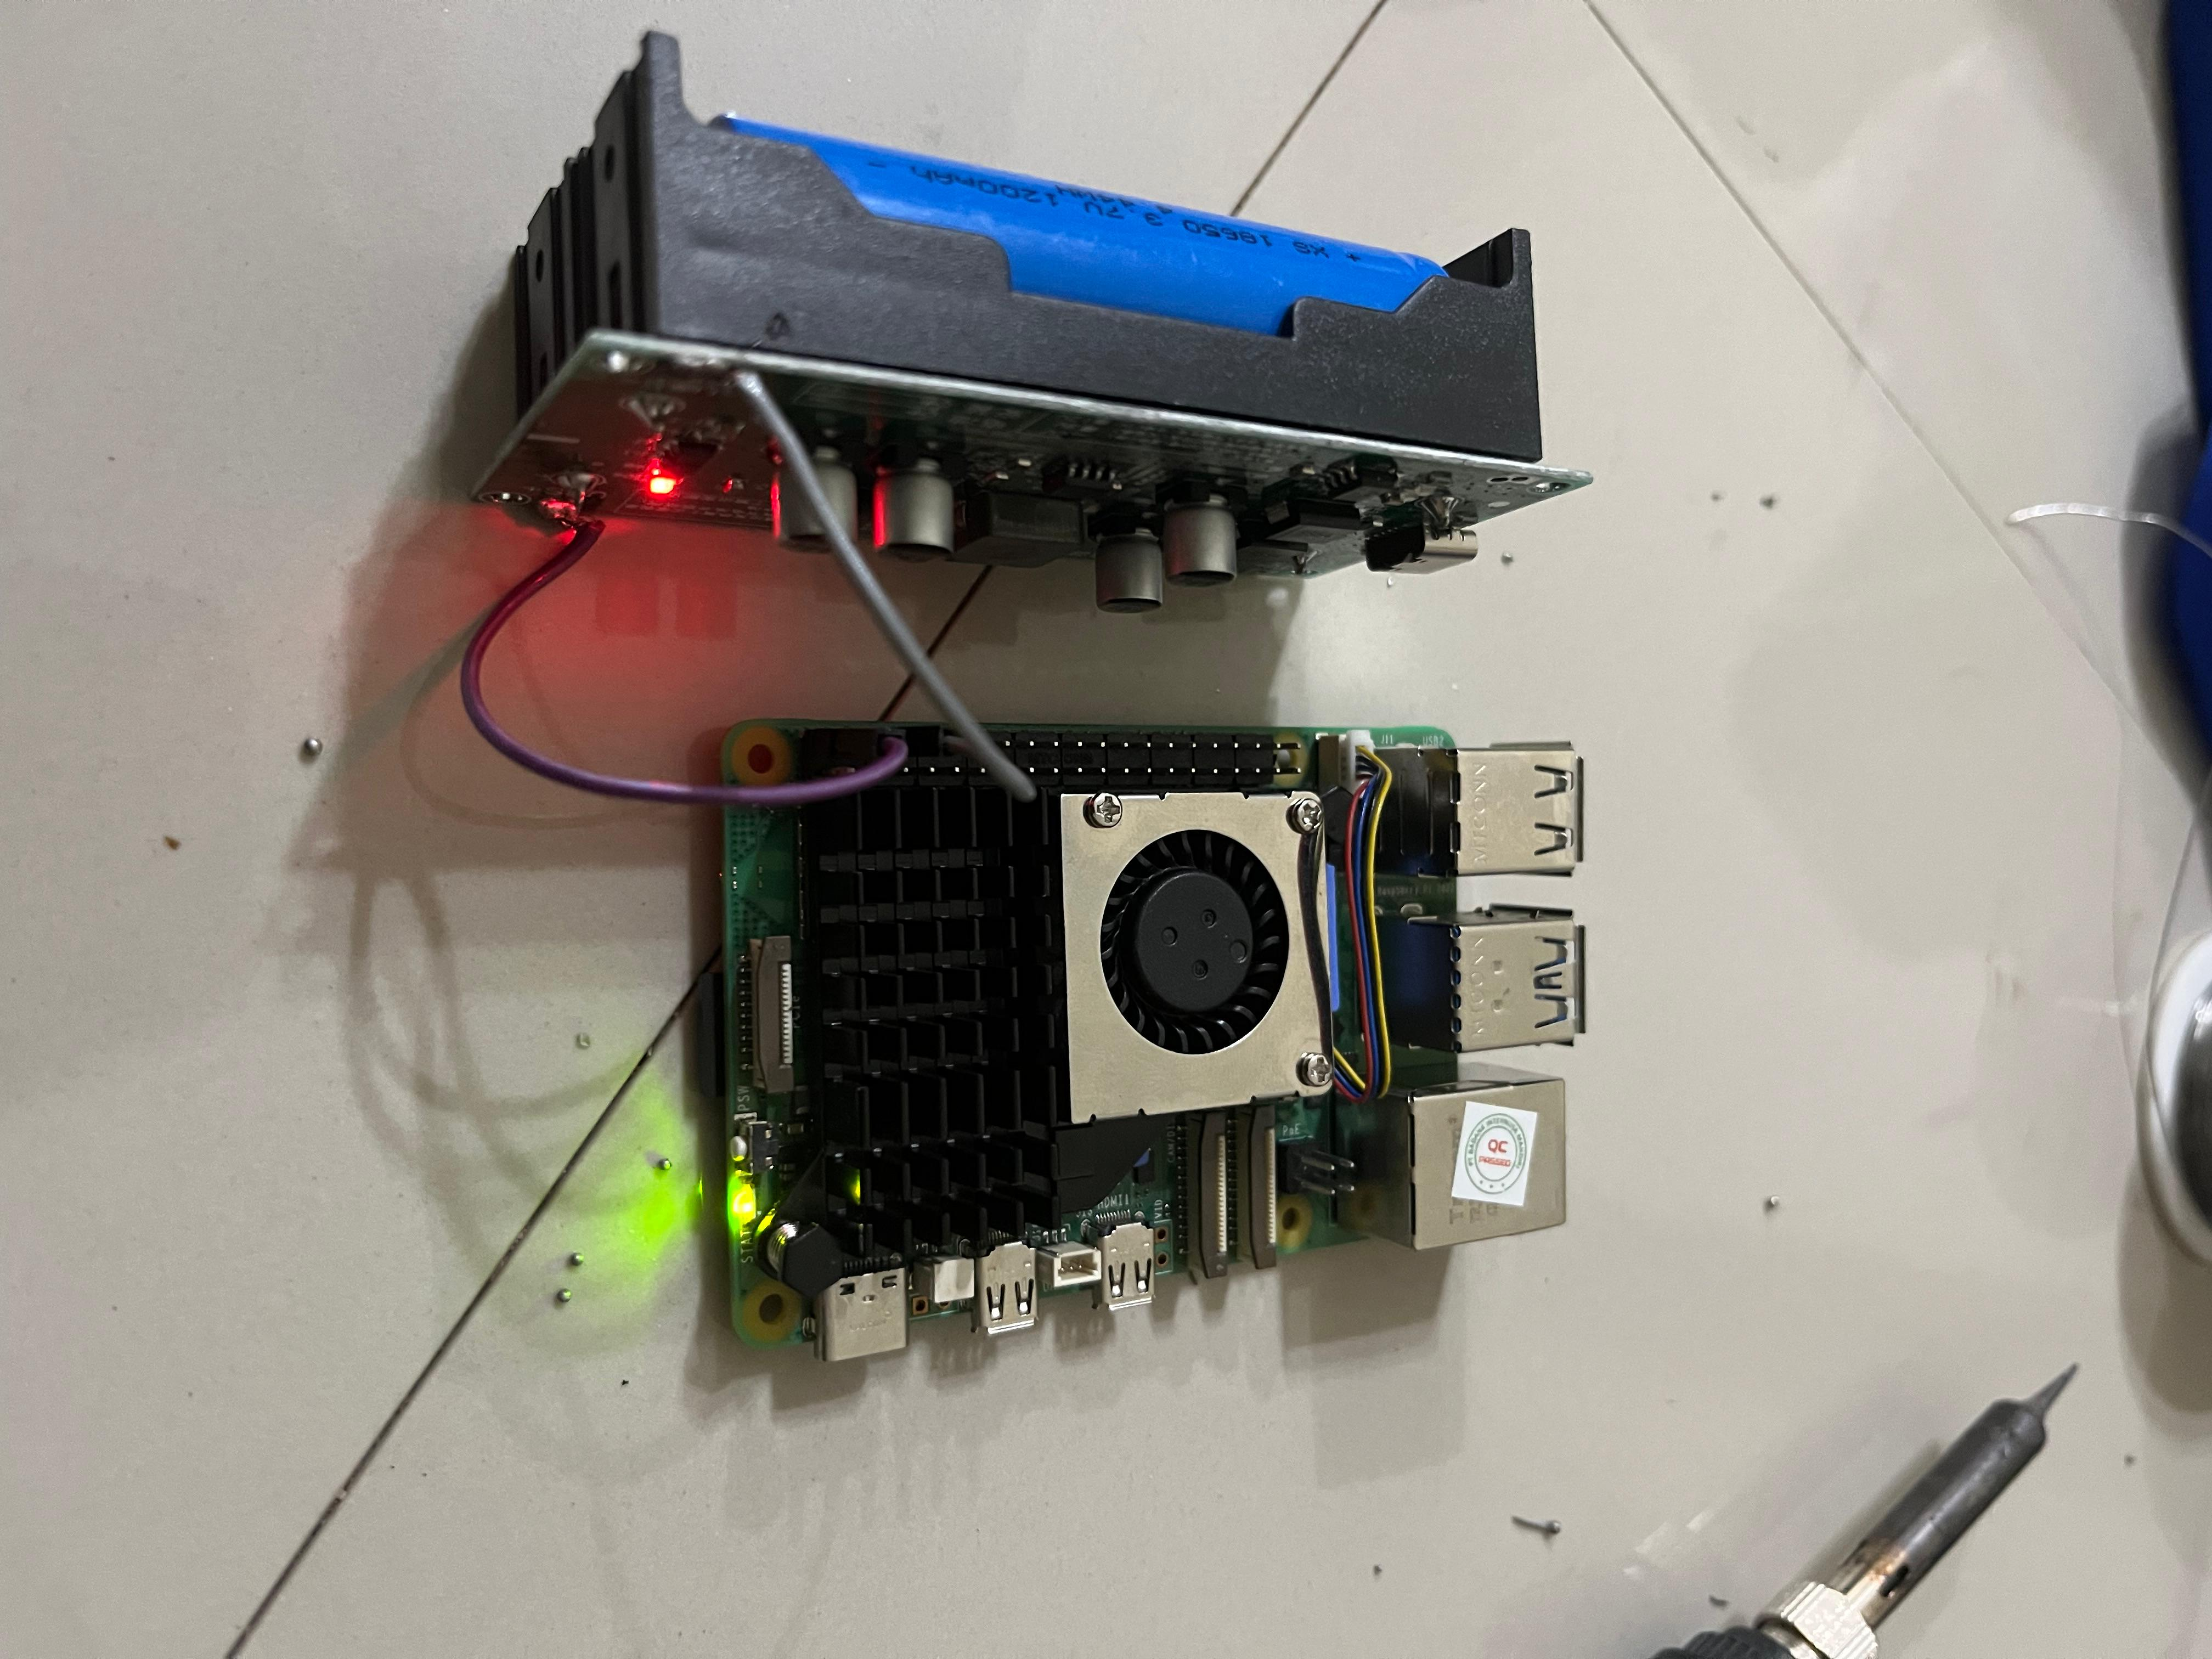
\includegraphics[width=0.6\linewidth]{bab4/korslet_pi5}
		\caption{Insiden Korsleting pada Raspberry Pi 5}
		\label{fig:korsletingpi5}
	\end{figure}
	Pada uji coba fase pertama menggunakan modul Mini UPS melalui pin ekspansi GPIO (sebagaimana ditunjukkan pada Gambar \ref{fig:korsletingpi5}), sistem mengalami kegagalan booting permanen. Ketika model YOLOv8 melakukan inisialisasi beban kerja (\textit{startup spike}), terjadi lonjakan arus transien yang radikal. Karena pin GPIO Raspberry Pi 5 tidak dilengkapi sirkuit proteksi internal seperti \textit{Over-Voltage Protection} (OVP) atau \textit{Over-Current Protection} (OCP), lonjakan ini memicu kondisi arus pendek (\textit{short circuit}) ringan yang langsung merusak PMIC (\textit{Power Management Integrated Circuit}) \textit{board}. Kegagalan ini divalidasi oleh indikator LED diagnostik yang menyala merah kaku (\textit{stuck red LED}).
	
	\item Analisis Gejala \textit{Throttling} 0x5000 (Modul XL4015E1):
	\begin{figure}[H]
		\centering
		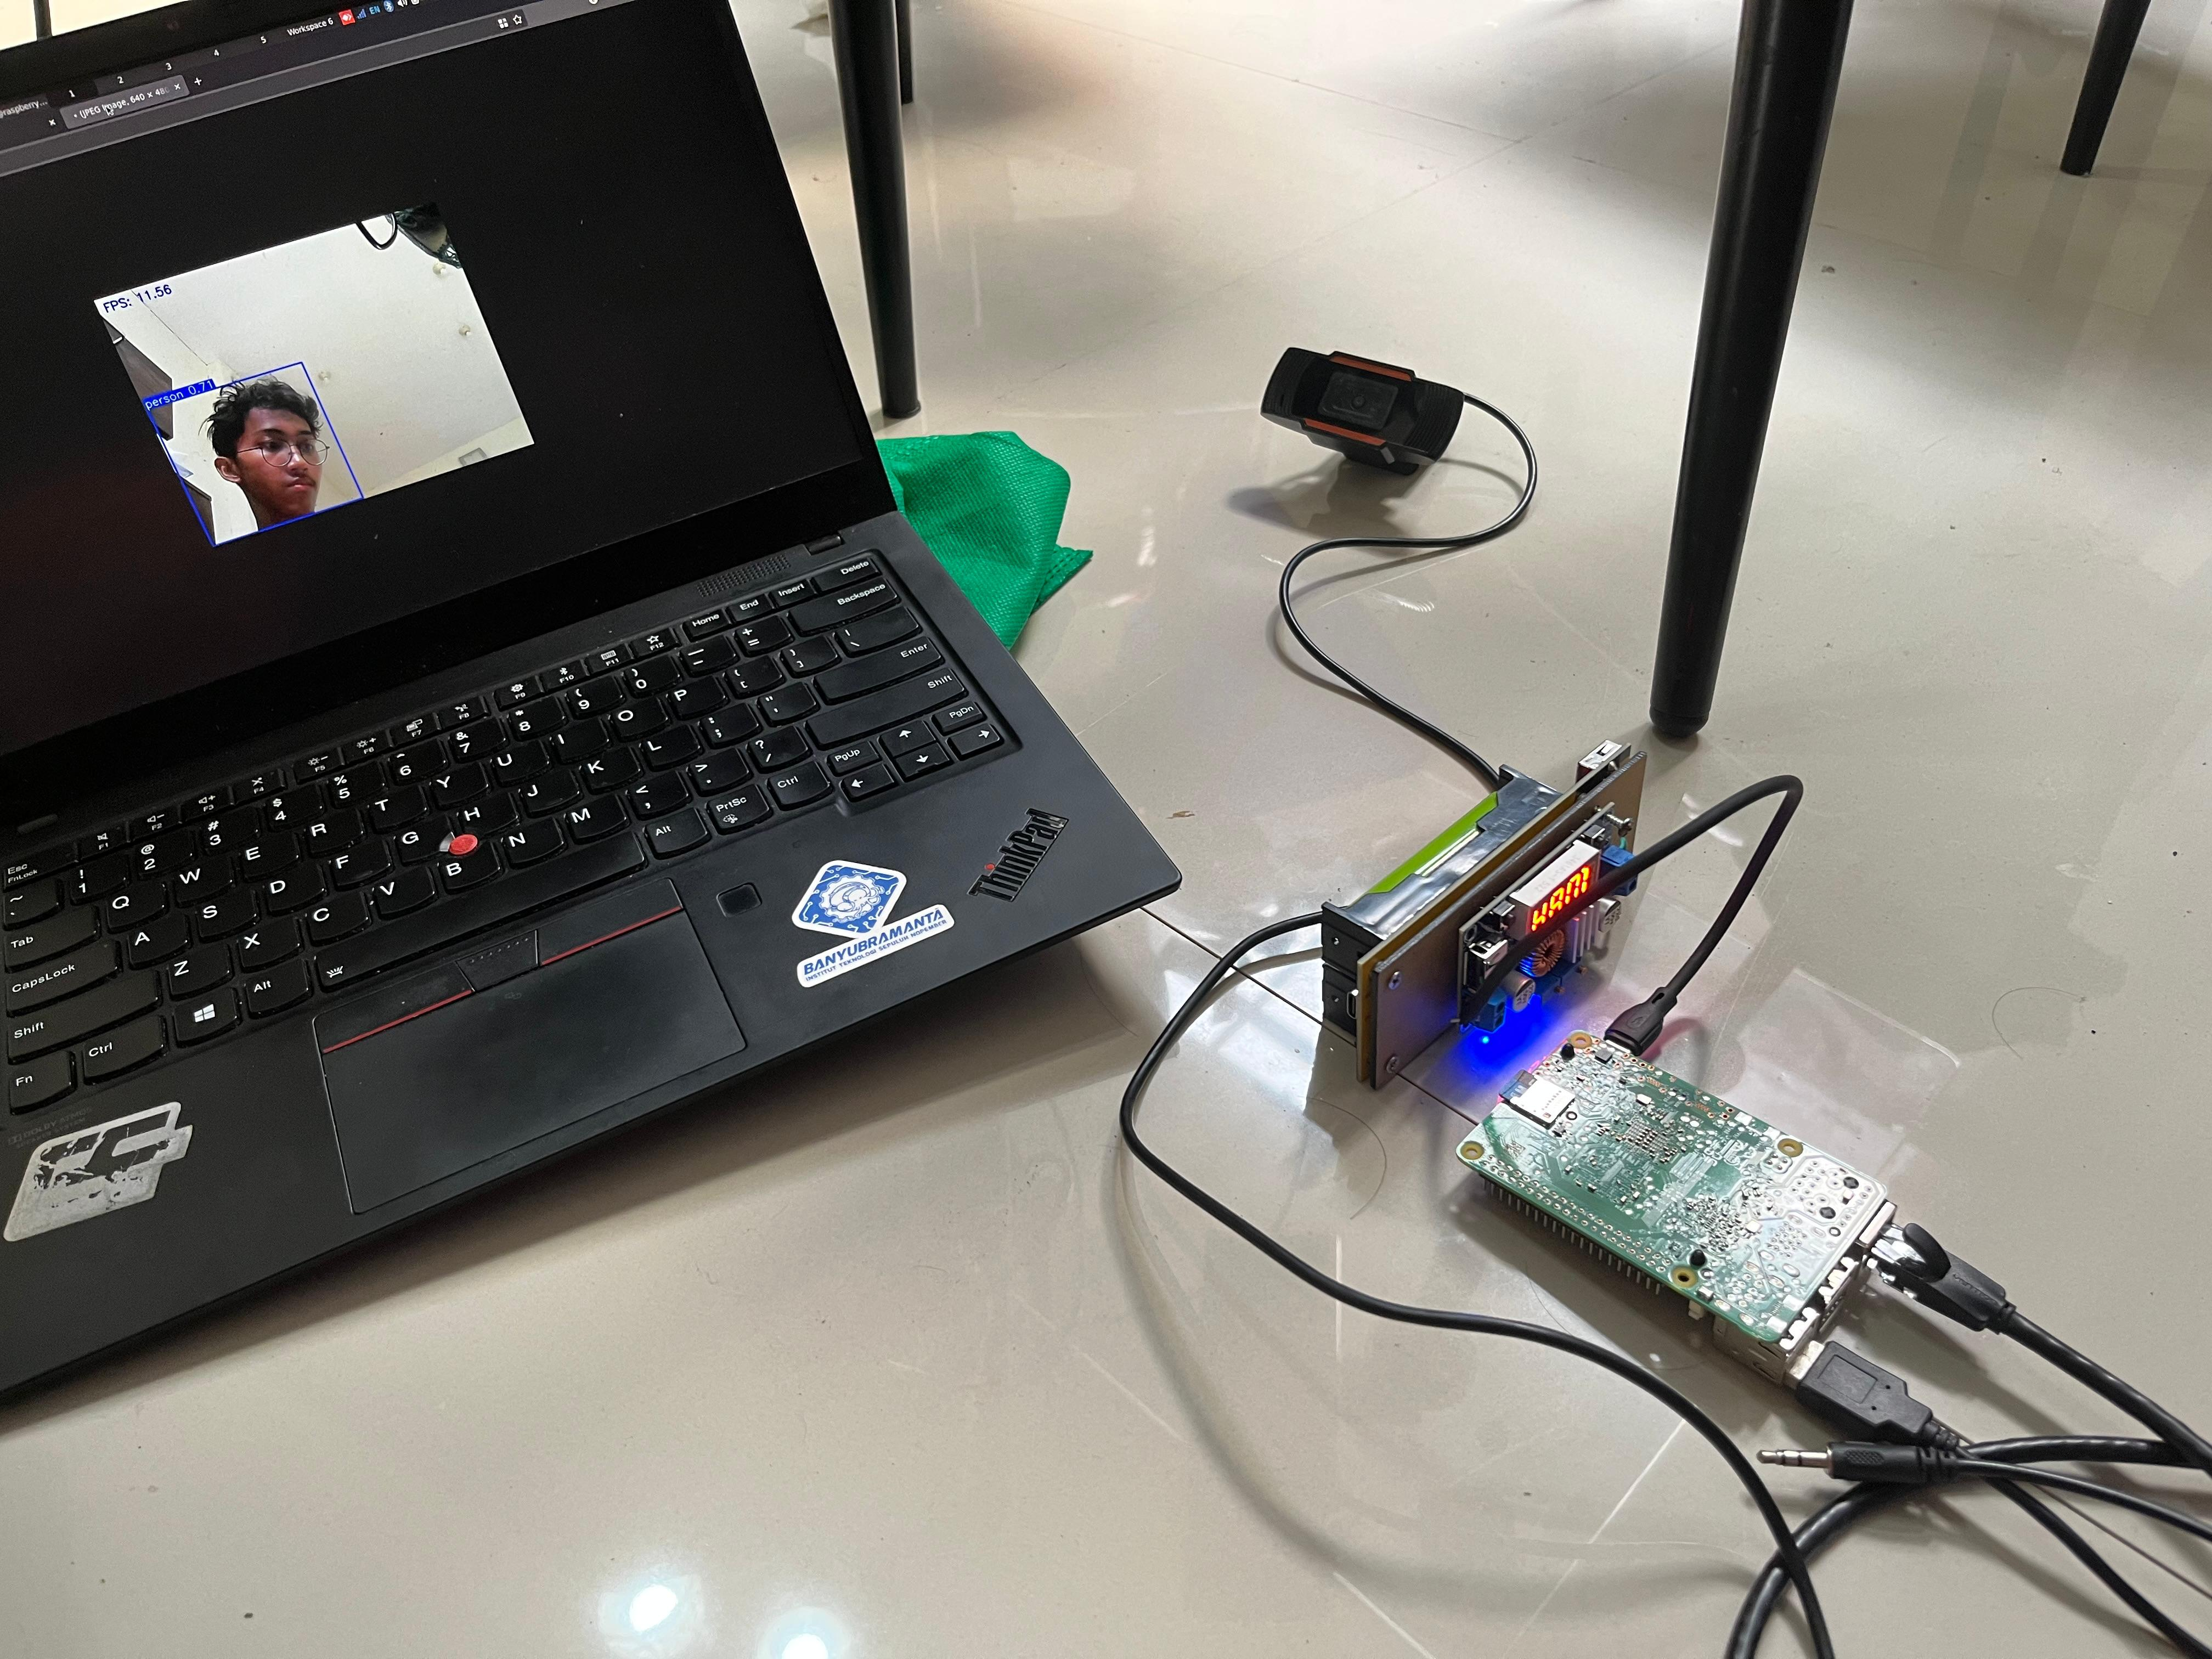
\includegraphics[width=0.6\linewidth]{bab4/throttle_pi5}
		\caption{Insiden Throttling pada Raspberry Pi 5}
		\label{fig:throttlingxl4015e1}
	\end{figure}
	Pengujian diturunkan menggunakan regulator XL4015E1 (Gambar \ref{fig:throttlingxl4015e1}). Meskipun Raspberry Pi 5 berhasil melakukan booting dan menjalankan program ringan (satu utas deteksi), perangkat mengalami \textit{reboot} otomatis secara berkala. Log kernel mendeteksi kesalahan kode 0x5000 (\textit{Under-voltage has occurred}). Walaupun modul XL4015E1 memiliki batas nominal 5A, respons transien induktornya terlalu lambat mengompensasi fluktuasi beban digital, sehingga tegangan turun di bawah 4,63V dan memicu restart pengamanan.
	
	\item Analisis \textit{Power Drop} akibat Karakteristik Baterai (Modul XL4016E1): 
	Untuk mengatasi \textit{under-voltage}, pengujian beralih ke modul XL4016E1 (8A). Kondisi awal menunjukkan performa yang sangat stabil pada saat sistem berada dalam posisi \textit{idle}. Namun, seketika program otonom dieksekusi secara utuh \textit{pipeline} video GStreamer aktif, MAVSDK melakukan \textit{polling} data, dan model YOLOv8 menginferensi citra secara paralel mengakibatkan Raspberry Pi 5 langsung mati total (\textit{blackout}). Masalah ini bersumber dari keterbatasan baterai Li-ion 18650 standar yang memiliki nilai \textit{continuous discharge rate} (C-rating) yang rendah. Ketika sirkuit otonom meminta lonjakan arus masif secara mendadak, sel baterai mengalami \textit{drop} tegangan internal yang drastis (\textit{voltage sag}) \cite{mcnulty2022_liion_review}, sehingga XL4016E1 kehilangan tegangan input minimal untuk meregulasi daya keluaran.
\end{enumerate}

Sebagai solusi akhir untuk mengatasi seluruh kendala tersebut, sistem direvisi menggunakan UBEC 5A yang dihubungkan langsung ke baterai LiPo utama drone melalui konektor XT60 \textit{Y-Splitter}. Konfigurasi ini terbukti berhasil mempertahankan tegangan suplai secara stabil meskipun inferensi AI dan operasi penerbangan drone berlangsung secara bersamaan.
\section{Optimasi Lingkungan Sistem Operasi Edge Computing}

Pengujian dilakukan untuk mengevaluasi pengaruh lingkungan sistem operasi terhadap performa inferensi AI pada Raspberry Pi 5. Pemilihan konfigurasi sistem operasi yang tepat menjadi parameter krusial untuk meminimalisir penggunaan RAM dan CPU oleh proses latar belakang. Dengan demikian, alokasi sumber daya komputasi dapat diprioritaskan secara penuh untuk pemrosesan citra \textit{real-time} dan komunikasi navigasi.

\subsection{Perbandingan Mode Desktop dan Headless}

Perbandingan penggunaan sistem operasi desktop dan headless ditunjukkan pada Tabel \ref{tab:headless_compare}. Pengukuran dilakukan pada parameter utilisasi memori, kestabilan frame rate, serta beban CPU saat platform berada pada kondisi idle maupun beban kerja penuh. Hasil komparasi ini digunakan untuk meningkatkan efisiensi runtime arsitektur otonom drone.

\begin{table}[H]
	\centering
	\caption{Perbandingan Sistem Operasi Desktop dan Headless}
	\label{tab:headless_compare}
	\renewcommand{\arraystretch}{1.2}
	\begin{tabular}{|p{3cm}|p{2.5cm}|p{2.5cm}|p{2.5cm}|p{3cm}|}
		\hline
		Mode Sistem & RAM Idle & CPU Idle & FPS Inferensi & Stabilitas Sistem \\ \hline
		
		Desktop &
		$\sim$1.2 GB &
		Tinggi &
		Tidak stabil &
		Frame drop dan latensi meningkat \\ \hline
		
		Headless &
		$\sim$420 MB &
		Lebih rendah &
		Stabil &
		Respons inferensi lebih konsisten \\ \hline
	\end{tabular}
\end{table}

Hasil pengujian menunjukkan mode \textit{headless} mengonsumsi sumber daya yang jauh lebih rendah dibanding mode desktop. Peniadaan antarmuka grafis membuat inferensi ONNX Runtime pada Raspberry Pi 5 lebih stabil. Selain mengurangi proses latar belakang sistem operasi, optimasi ini memfokuskan alokasi CPU dan RAM untuk inferensi visual, telemetri MAVSDK, serta streaming video.

Optimasi sirkuit operasi pada level sistem operasi ini memberikan fondasi penting bagi efisiensi komputasi visual. Selanjutnya, performa platform diuji menggunakan beberapa variasi model kecerdasan buatan untuk menentukan arsitektur pendeteksi yang paling optimal sebelum memasuki tahapan pelatihan khusus.

\section{Pengujian Komparatif Model Deteksi Manusia}

Sebelum melakukan proses \textit{fine-tuning} model, penelitian ini terlebih dahulu melakukan pengujian komparatif terhadap beberapa konfigurasi model deteksi manusia untuk menentukan base model yang paling sesuai digunakan pada Raspberry Pi 5.
Tahap ini bertujuan untuk mengevaluasi pengaruh arsitektur model, penggunaan pose estimation, dan resolusi inferensi terhadap performa \textit{real-time} pada platform \textit{edge computing}.
Hasil pengujian awal ini kemudian digunakan sebagai dasar pemilihan model utama yang akan digunakan pada proses \textit{fine-tuning} khusus kelas manusia.
Model yang dibandingkan meliputi:

\begin{itemize}
	\item YOLOv8n original,
	\item YOLOv8n-pose,
	\item resolusi inferensi 256×256,
	\item resolusi inferensi 320×320,
	\item dan resolusi inferensi 640×640.
\end{itemize}

Pengujian performa model deteksi manusia ini dilakukan pada kondisi \textit{indoor} dan \textit{outdoor} dengan membatasi jarak deteksi antara 2 hingga 5 meter. Evaluasi difokuskan terhadap parameter inferensi \textit{real-time}, latensi komputasi, kestabilan kotak pembatas (\textit{bounding box}), konsistensi deteksi antar-frame, serta pemanfaatan sumber daya komputasi Raspberry Pi 5.

\subsection{Perbandingan YOLOv8n dan YOLOv8n-Pose}

YOLOv8n-pose dipilih sebagai salah satu model pembanding karena memiliki kemampuan estimasi pose tubuh manusia menggunakan keypoint detection.
Namun demikian, kompleksitas tambahan pada proses inferensi menyebabkan beban komputasi model meningkat dibandingkan YOLOv8n original.
Selain itu, kebutuhan utama sistem drone otonom pada penelitian ini berfokus pada deteksi keberadaan manusia secara \textit{real-time}, bukan analisis pose tubuh secara detail.
Oleh karena itu, penggunaan model pose estimation dinilai menghasilkan beban komputasi tambahan yang kurang efisien untuk platform \textit{edge computing} berbasis Raspberry Pi 5.

Pengujian awal dilakukan menggunakan empat konfigurasi model ONNX sebagaimana ditunjukkan pada Tabel \ref{tab:model_compare_awal}. Skenario pengujian ini mengukur performa kecepatan pemrosesan dalam satuan frame per second (FPS) dan waktu latensi inferensi. Data awal ini menjadi parameter dasar untuk mengevaluasi efisiensi komputasi visual pada companion computer.

\begin{table}[H]
	\centering
	\caption{Perbandingan Awal Model YOLOv8n dan YOLOv8n-Pose}
	\label{tab:model_compare_awal}
	\renewcommand{\arraystretch}{1.2}
	\begin{tabular}{|p{5cm}|c|c|}
		\hline
		Model & FPS (avg) & Inferensi (ms) \\ \hline
		
		YOLOv8n 256 &
		17.67 &
		46.16 \\ \hline
		
		YOLOv8n 320 &
		15.08 &
		65.39 \\ \hline
		
		YOLOv8n 256 Pose &
		18.08 &
		43.92 \\ \hline
		
		YOLOv8n 320 Pose &
		14.70 &
		62.81 \\ \hline
	\end{tabular}
\end{table}

Data pada Tabel \ref{tab:model_compare_awal} menunjukkan bahwa resolusi input memiliki pengaruh yang lebih signifikan terhadap performa komputasi dibandingkan variasi jenis model (standar vs pose). Pengurangan resolusi dari 320 ke 256 piksel mampu meningkatkan \textit{frame rate} rata-rata sebesar 17\%--22\% serta meredam latensi inferensi hingga di bawah 50 ms. Implikasi dari hasil ini adalah konfigurasi resolusi yang lebih rendah dapat memberikan kelonggaran beban CPU (\textit{headroom}) pada Raspberry Pi 5 yang sangat krusial untuk menjaga stabilitas sirkuit kontrol navigasi otonom yang berjalan secara paralel.

Untuk memastikan hasil pengujian bersifat konsisten dan tidak dipengaruhi fluktuasi sesaat pada sistem operasi Raspberry Pi 5, dilakukan pengujian ulang menggunakan skenario identik sebagaimana ditunjukkan pada Tabel \ref{tab:model_compare_awal2}.

\begin{table}[H]
	\centering
	\caption{Pengujian Ulang Perbandingan Model YOLOv8n dan YOLOv8n-Pose}
	\label{tab:model_compare_awal2}
	\renewcommand{\arraystretch}{1.2}
	\begin{tabular}{|p{5cm}|c|c|}
		\hline
		Model & FPS (avg) & Latensi (ms) \\ \hline
		
		YOLOv8n 256 &
		18,02 &
		49,10 \\ \hline
		
		YOLOv8n 320 &
		15,21 &
		63,30 \\ \hline
		
		YOLOv8n 256 Pose &
		18,18 &
		44,67 \\ \hline
		
		YOLOv8n 320 Pose &
		14,70 &
		63,12 \\ \hline
	\end{tabular}
\end{table}

Berdasarkan hasil pengujian awal dan pengujian ulang, performa inferensi seluruh model relatif konsisten.
Model dengan resolusi 256×256 menghasilkan FPS lebih tinggi dibandingkan resolusi 320×320 karena ukuran input citra lebih kecil sehingga jumlah operasi komputasi yang diproses ONNX Runtime menjadi lebih rendah.
Meskipun model YOLOv8n-pose memiliki FPS yang relatif mirip dengan YOLOv8n original, pengamatan visual secara langsung menunjukkan bahwa model pose mengalami ketidakstabilan pada proses estimasi skeleton ketika dijalankan pada kondisi outdoor.

Pada pengujian outdoor dengan jarak sekitar 2--3 meter, model YOLOv8n256-pose menghasilkan rata-rata FPS sekitar 19--24 FPS dengan confidence deteksi berkisar antara 0,40 hingga 0,55. Namun demikian, sebagaimana ditunjukkan pada Gambar \ref{fig:outdoor_pose256}, skeleton pose dan \textit{bounding box} sering mengalami flickering atau hilang secara intermittently ketika objek manusia bergerak maupun ketika terjadi perubahan pencahayaan alami. Kondisi ini membuktikan bahwa penggunaan pose estimation pada lingkungan outdoor memiliki tantangan yang lebih tinggi akibat noise visual dan intensitas cahaya alami yang dinamis.

Sebaliknya, model YOLOv8n320 non-pose pada kondisi outdoor menghasilkan rata-rata FPS sekitar 23--25 FPS dengan confidence deteksi berkisar antara 0,41 hingga 0,60. Meskipun nilai confidence tidak meningkat secara signifikan, hasil visual pada Gambar \ref{fig:outdoor_320} menunjukkan bahwa kestabilan \textit{bounding box} yang dihasilkan terlihat lebih konsisten, lebih robust, dan tidak mudah hilang ketika objek manusia bergerak meskipun dijalankan pada lingkungan dengan perubahan perspektif kamera akibat pergerakan drone.

\begin{figure}[H]
	\centering
	\begin{minipage}{0.48\linewidth}
		\centering
		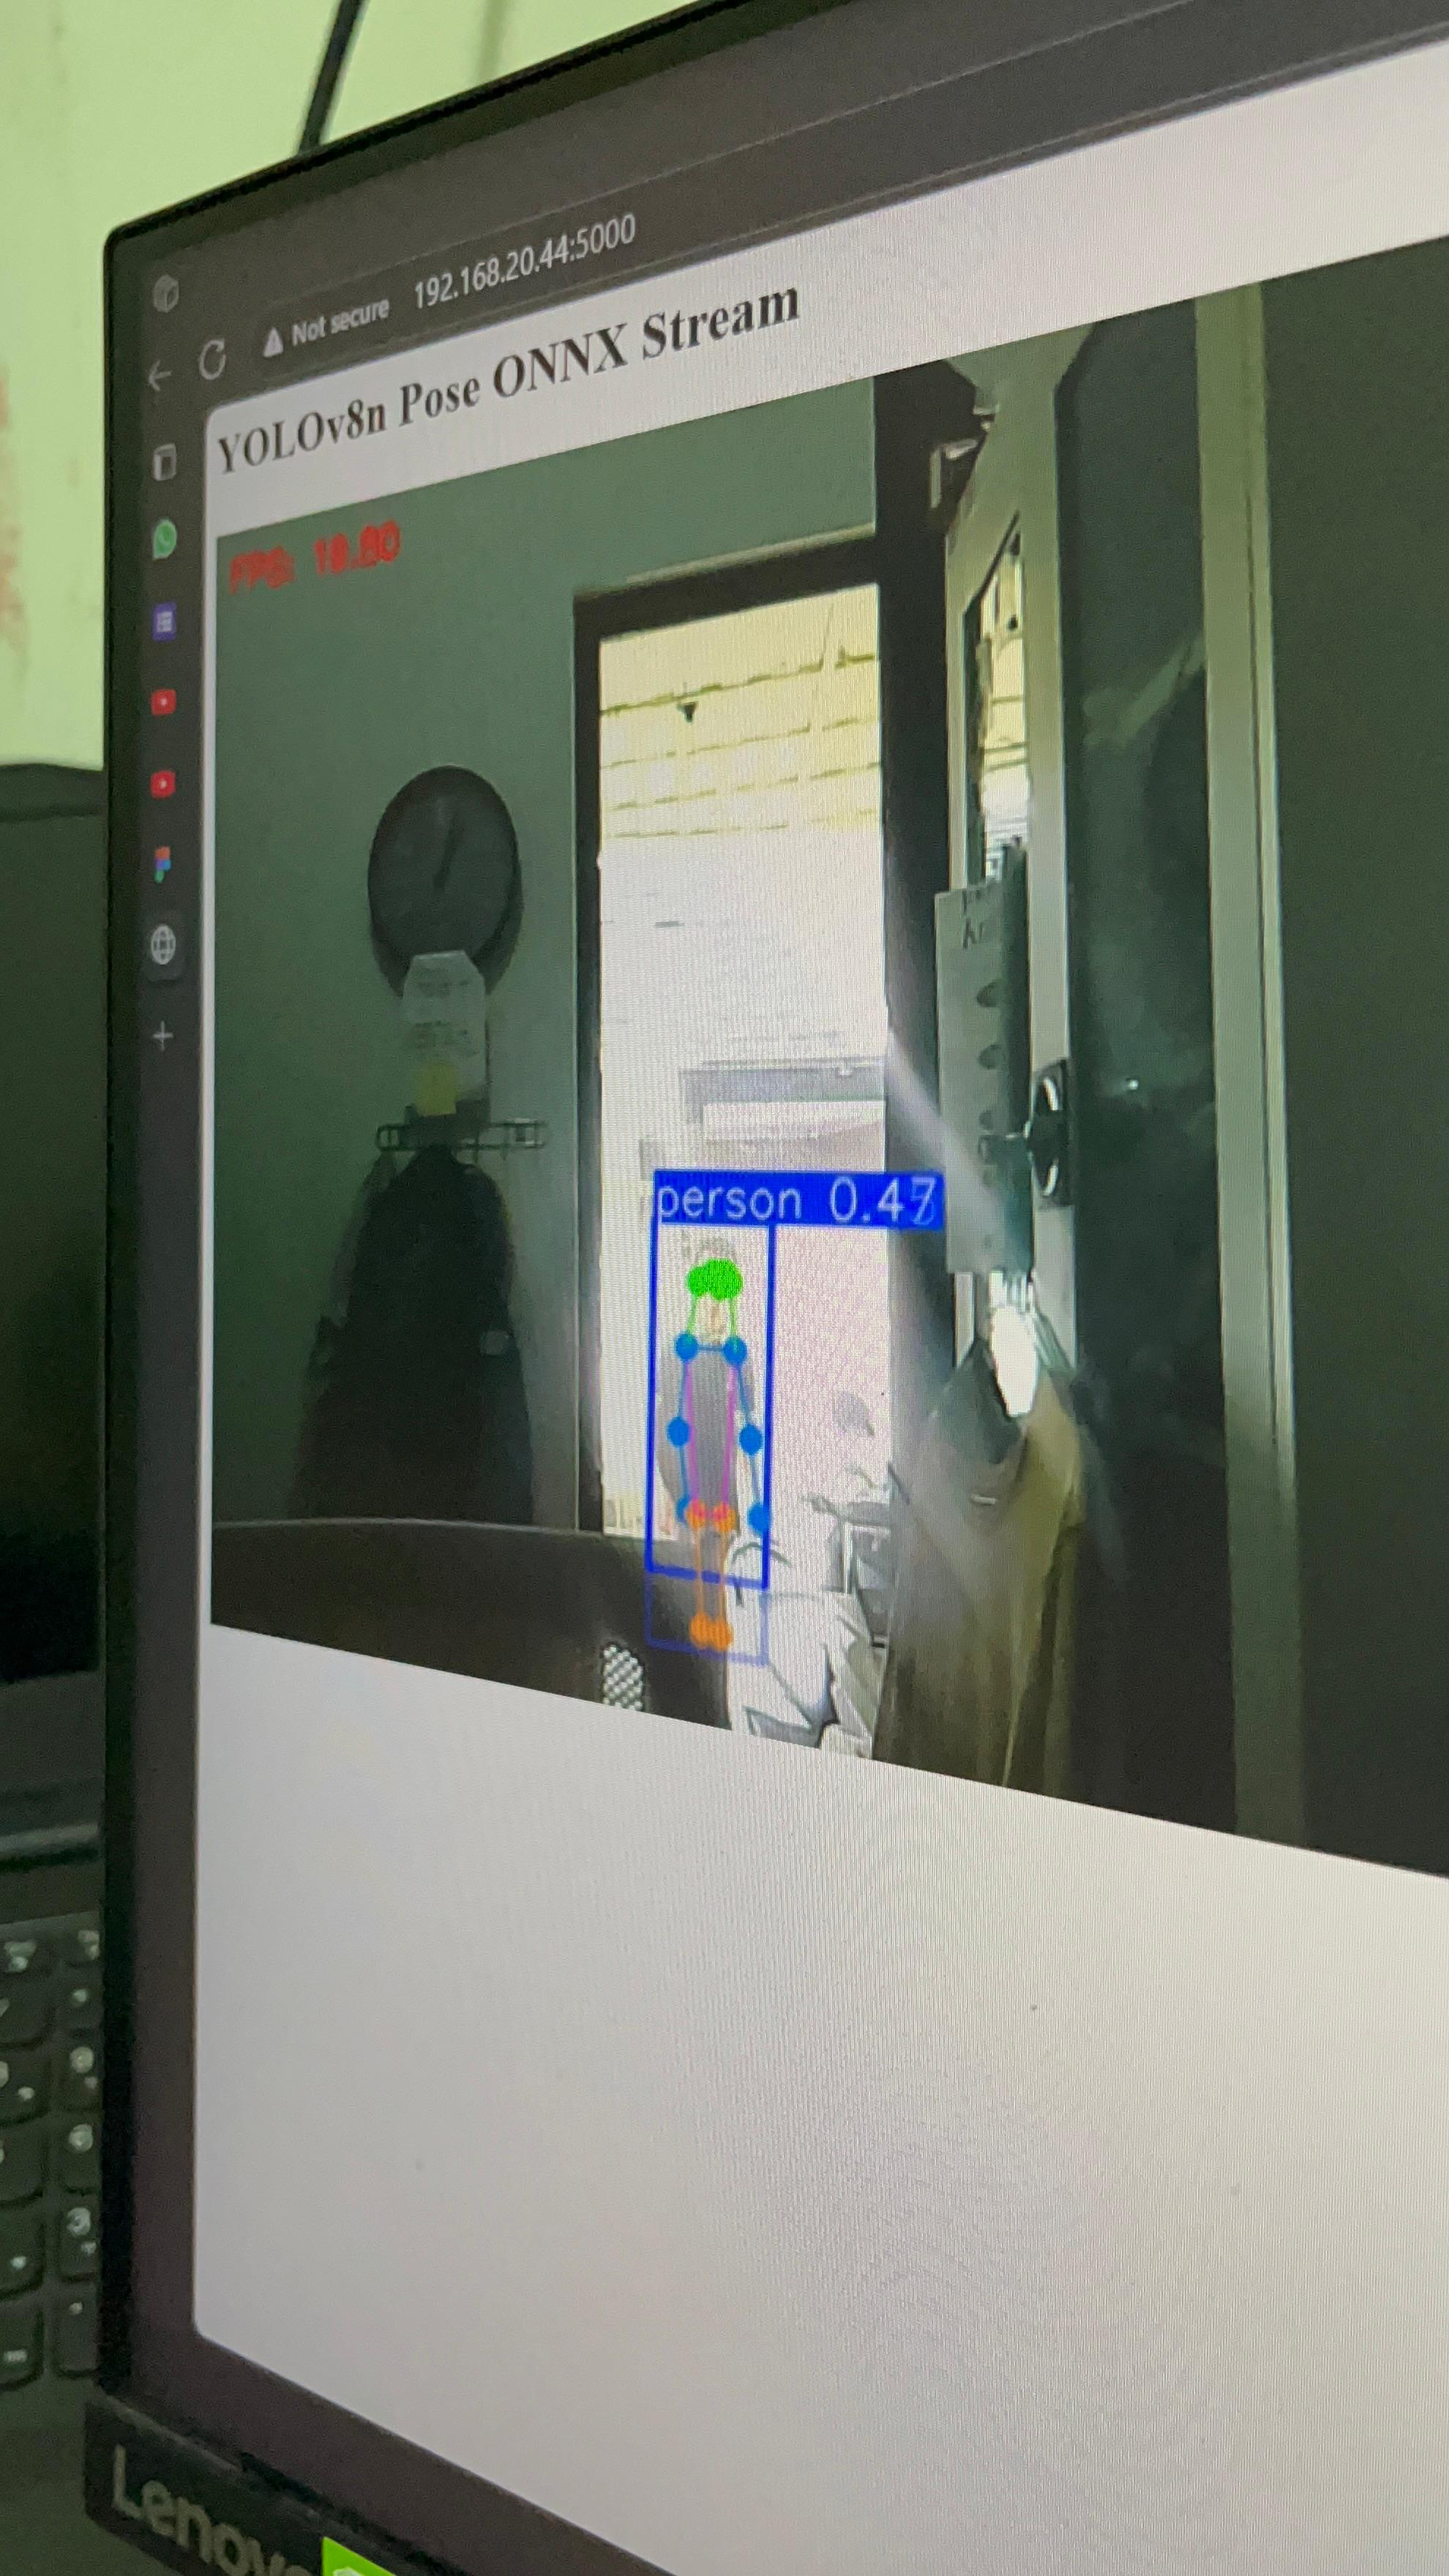
\includegraphics[width=\linewidth]{bab4/outdoor_yolov8n256_pose}
		\caption{Pengujian outdoor YOLOv8n256-pose ONNX pada Raspberry Pi 5}
		\label{fig:outdoor_pose256}
	\end{minipage}
	\hfill
	\begin{minipage}{0.48\linewidth}
		\centering
		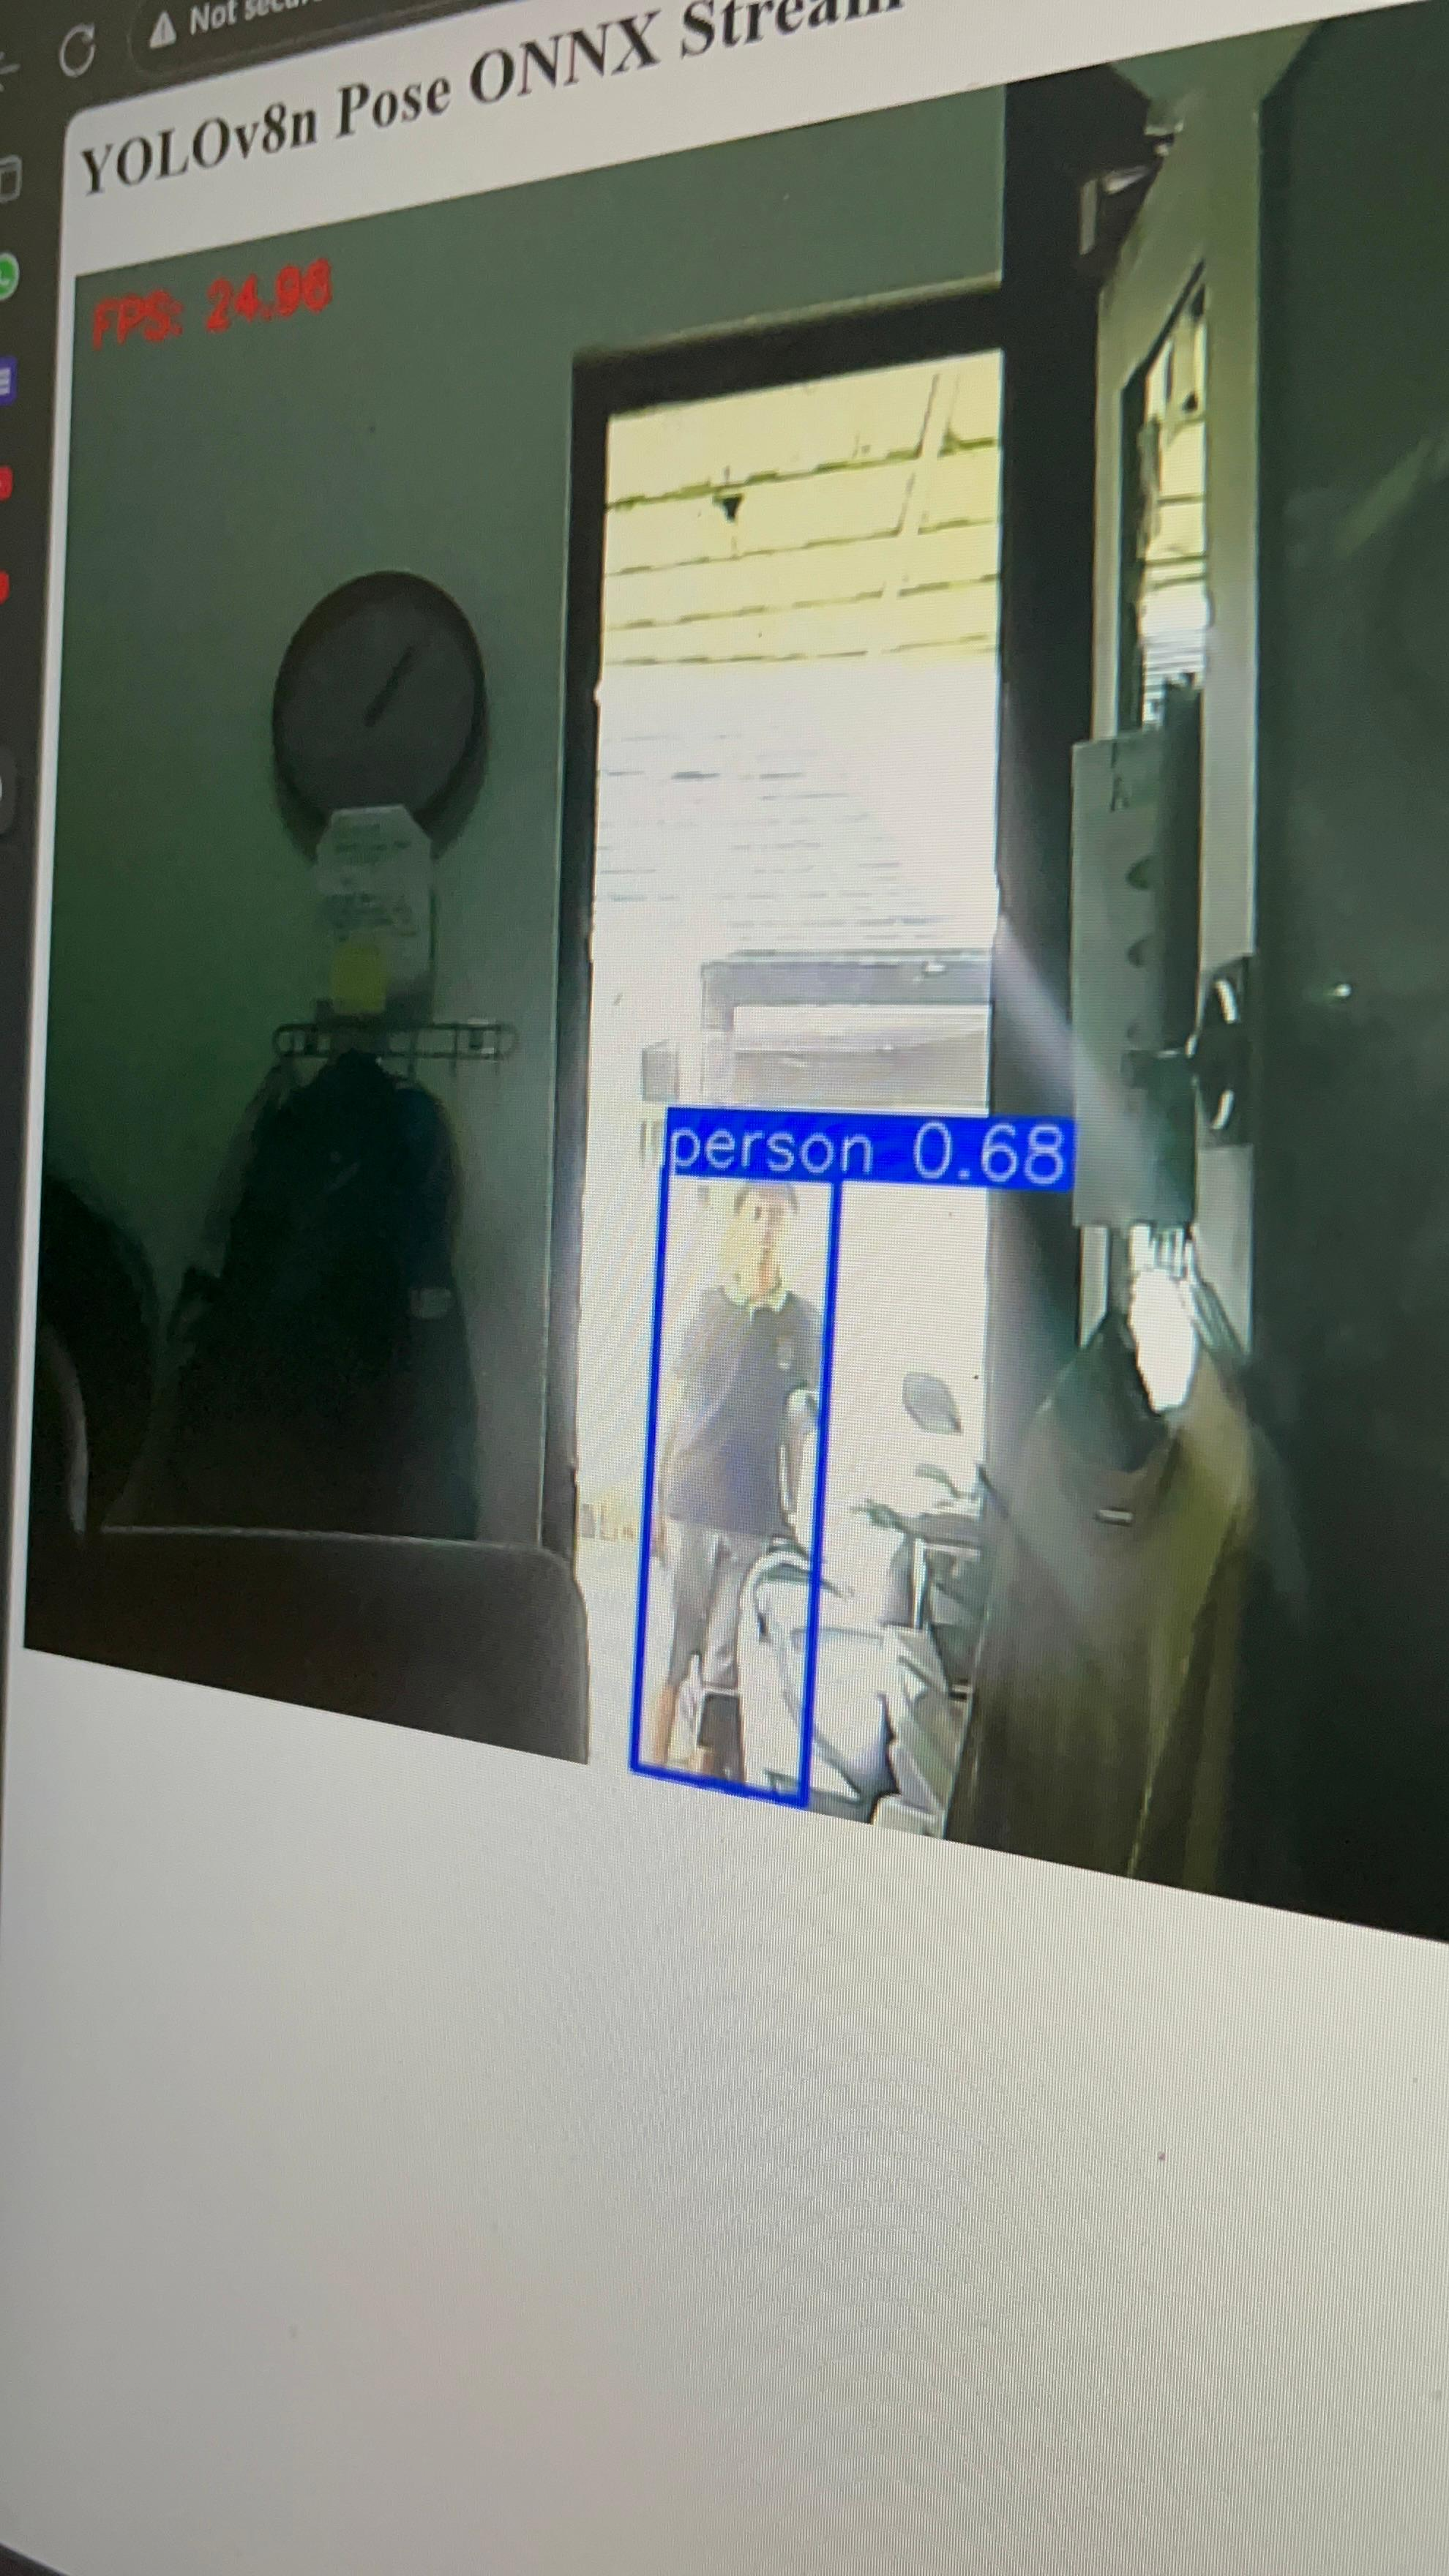
\includegraphics[width=\linewidth]{bab4/outdoor_yolov8n320}
		\caption{Pengujian outdoor YOLOv8n320 ONNX pada Raspberry Pi 5}
		\label{fig:outdoor_320}
	\end{minipage}
\end{figure}

Hasil tersebut menunjukkan estimasi pose pada platform \textit{edge} berbasis CPU masih terbatas untuk inferensi \textit{real-time}, khususnya di lingkungan luar ruang yang mengalami perubahan pencahayaan dinamis, \textit{motion blur}, dan pergeseran perspektif kamera.

Selain pengujian outdoor, dilakukan pula pengujian indoor dengan kondisi pencahayaan laboratorium yang relatif stabil untuk kedua jenis model tersebut. Hasil pengujian menunjukkan bahwa model YOLOv8n320 menghasilkan rata-rata FPS sekitar 20,25 FPS dengan latensi inferensi sekitar 38--39 ms dan confidence deteksi mencapai sekitar 0,85, dengan visualisasi kestabilan \textit{bounding box} yang ditunjukkan pada Gambar \ref{fig:indoor_320}. Pada pengujian yang sama, model YOLOv8n256 menghasilkan rata-rata FPS sekitar 27,66 FPS dengan latensi inferensi sekitar 25 ms dan confidence deteksi mencapai sekitar 0,88 sebagaimana ditampilkan pada Gambar \ref{fig:indoor_256}.

\begin{figure}[H]
	\centering
	\begin{minipage}{\textwidth}
		\centering
		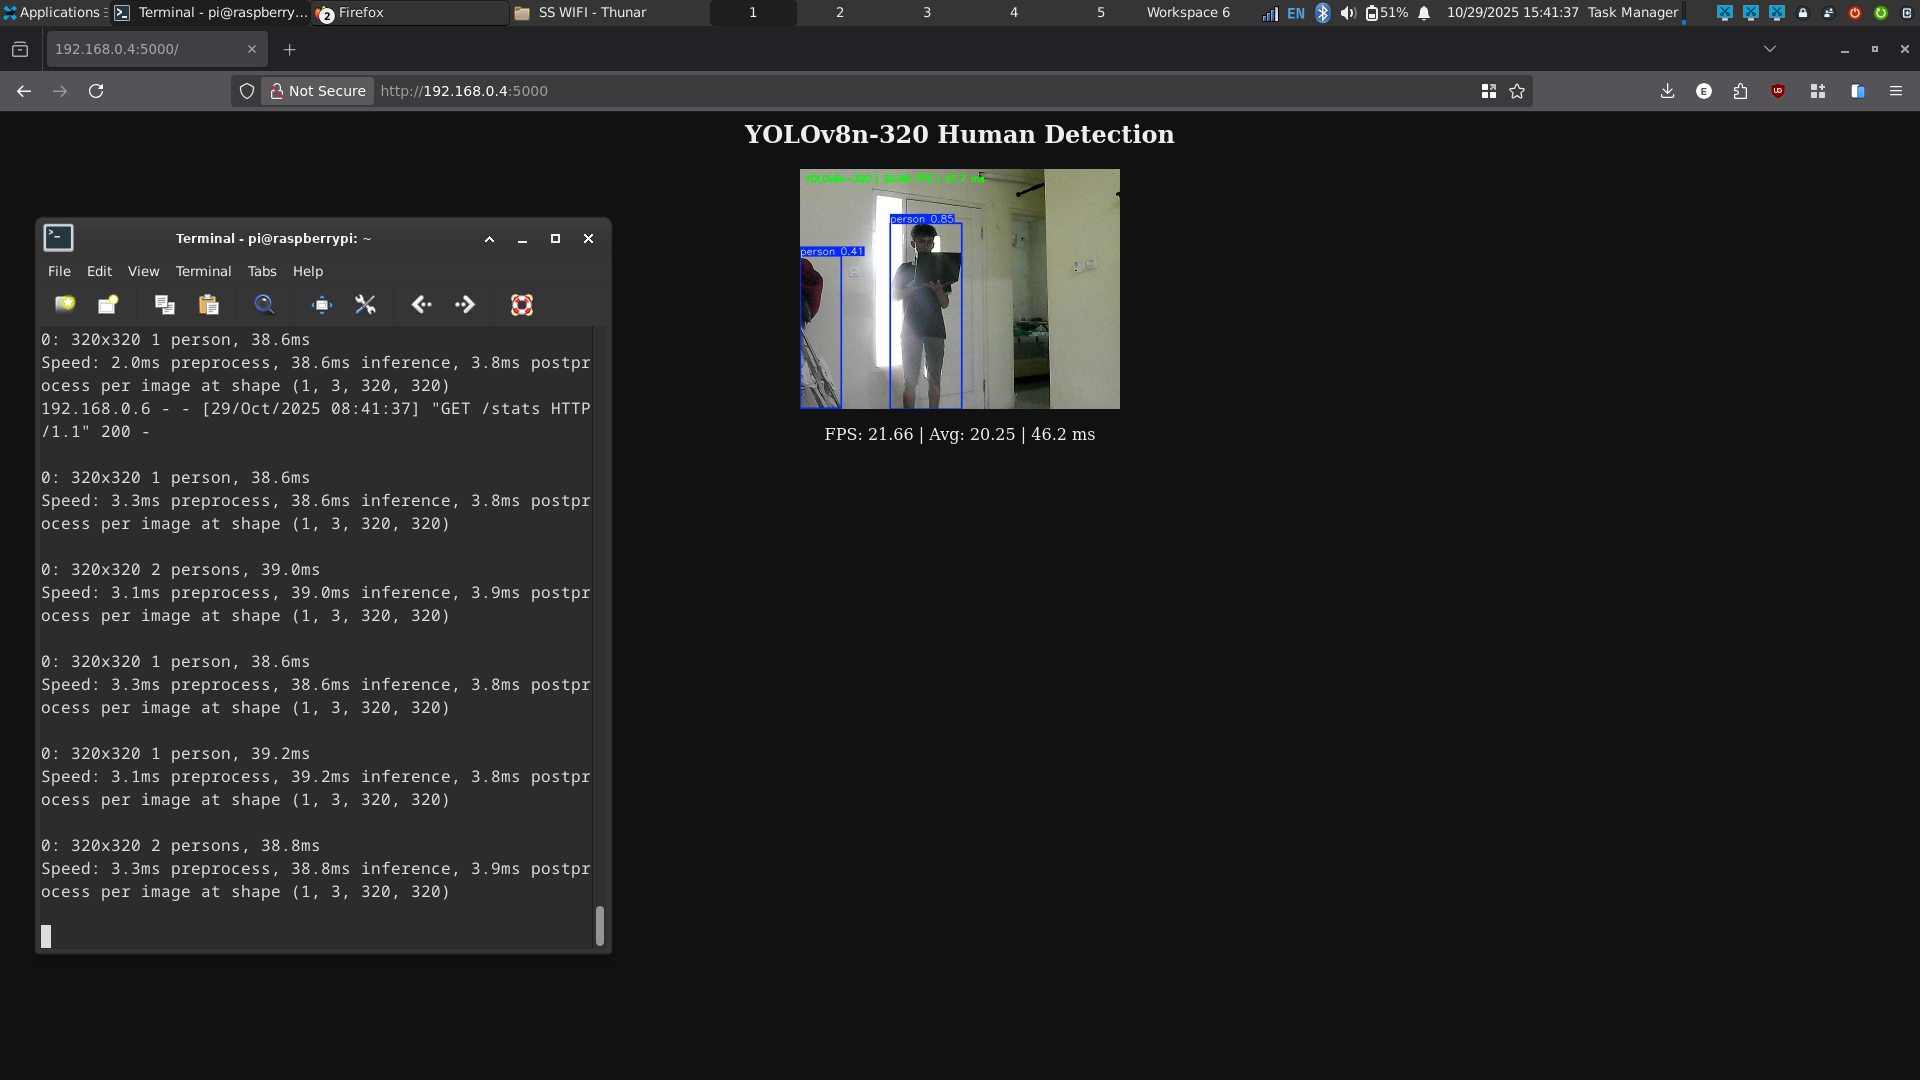
\includegraphics[width=\linewidth]{bab4/indoor_yolov8n320}
		\caption{Pengujian indoor YOLOv8n320 ONNX pada Raspberry Pi 5}
		\label{fig:indoor_320}
	\end{minipage}
	\hfill
	\begin{minipage}{\textwidth}
		\centering
		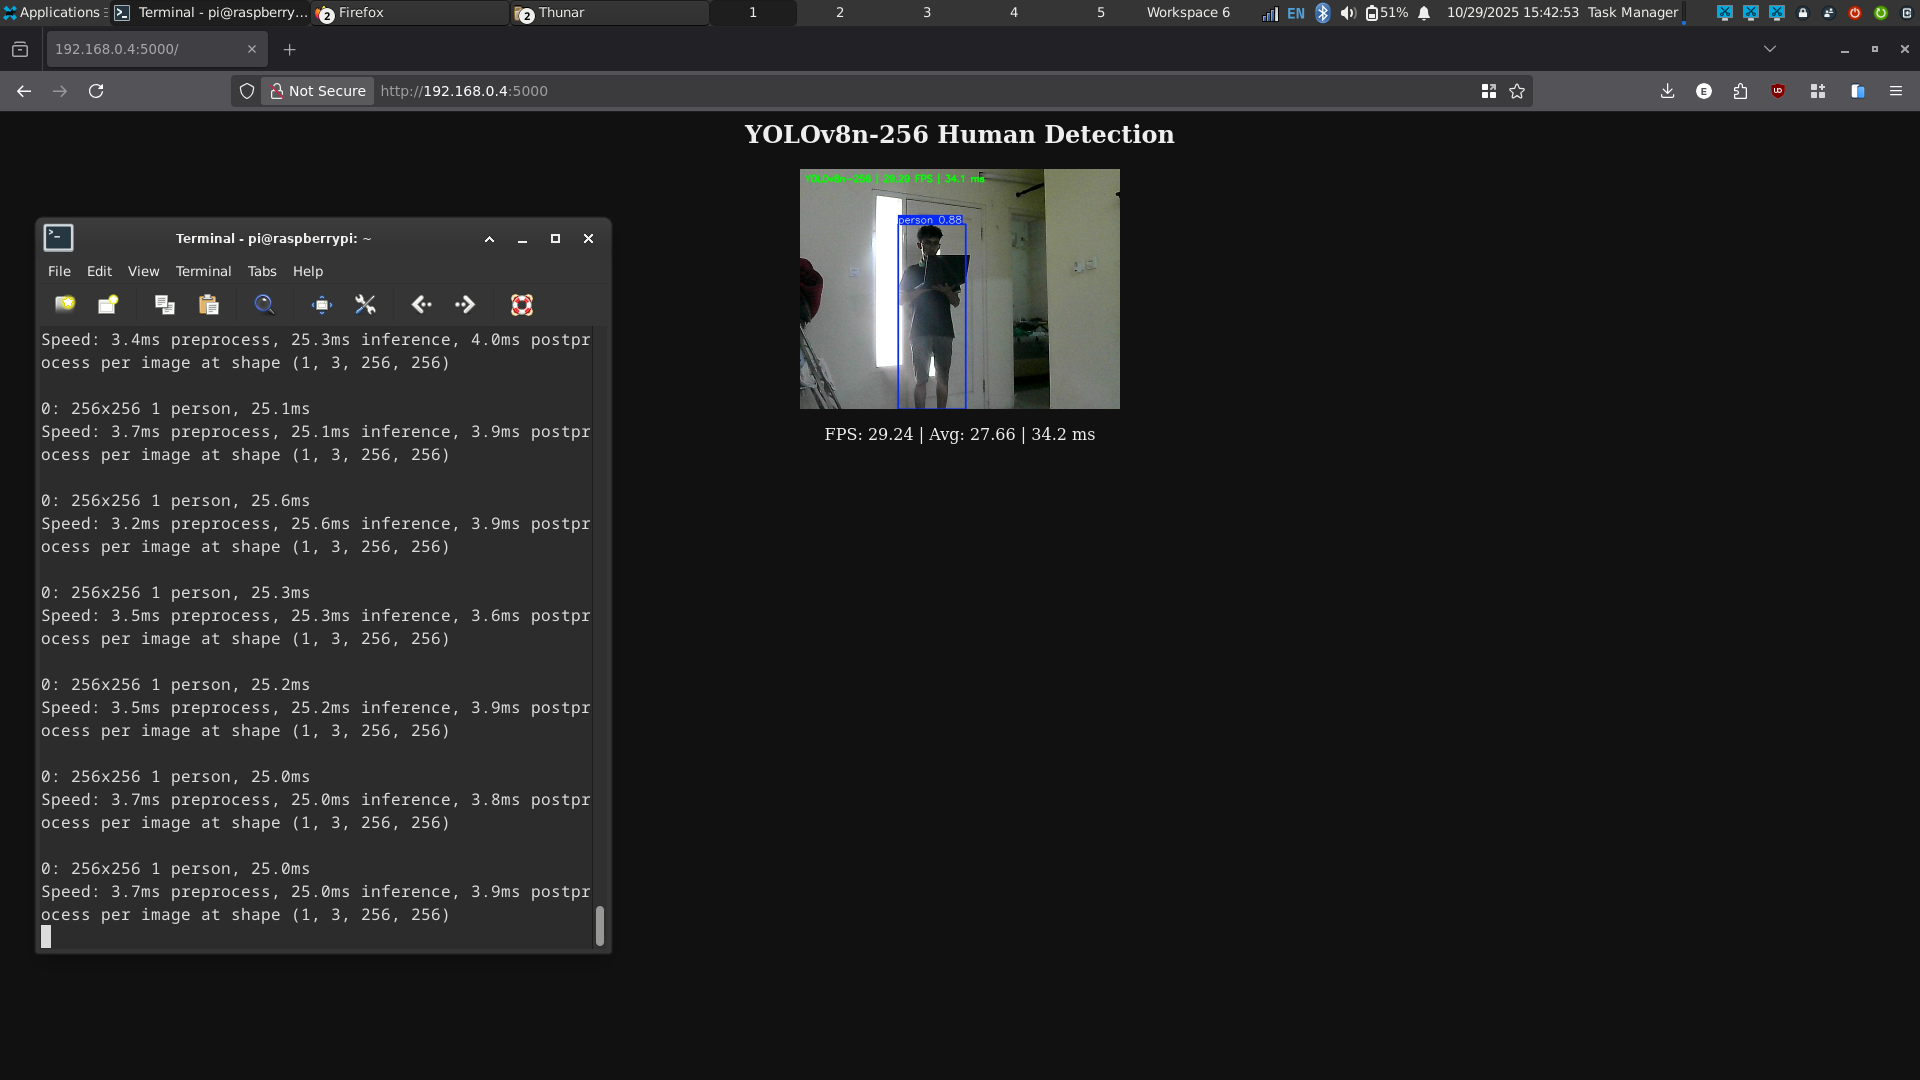
\includegraphics[width=\linewidth]{bab4/indoor_yolov8n256}
		\caption{Pengujian indoor YOLOv8n256 ONNX pada Raspberry Pi 5}
		\label{fig:indoor_256}
	\end{minipage}
\end{figure}

Meskipun resolusi 256×256 menghasilkan FPS lebih tinggi, pada beberapa kondisi tertentu kualitas detail \textit{bounding box} terlihat sedikit lebih rendah dibandingkan resolusi 320×320 terutama ketika objek manusia berada lebih jauh dari kamera. Secara umum, hasil pengujian indoor membuktikan bahwa seluruh model mampu bekerja lebih stabil karena lingkungan laboratorium memiliki pencahayaan lebih konstan, tingkat noise visual lebih rendah, dan pergerakan objek yang relatif lebih terkendali.

Meskipun demikian, pada implementasi sistem drone otonom nyata, kondisi outdoor tetap menjadi fokus utama penelitian karena operasi pencarian korban dilakukan pada area terbuka dengan kondisi lingkungan yang dinamis dan tidak terkontrol. Berdasarkan seluruh hasil pengujian tersebut, YOLOv8n original dinilai lebih sesuai digunakan sebagai base model dibandingkan YOLOv8n-pose karena memiliki kestabilan inferensi lebih baik pada kondisi operasi nyata meskipun tidak menyediakan fitur estimasi pose tubuh manusia.

\subsection{Analisis Pemilihan Model Final}

Berdasarkan seluruh hasil pengujian komparatif, penelitian ini memilih YOLOv8n original dengan resolusi inferensi 320×320 sebagai base model utama untuk proses \textit{fine-tuning}.
Keputusan tersebut didasarkan pada beberapa pertimbangan utama, yaitu:

\begin{itemize}
	\item performa inferensi lebih ringan,
	\item latensi lebih rendah,
	\item FPS lebih stabil,
	\item penggunaan memori lebih kecil,
	\item kestabilan \textit{bounding box} lebih baik,
	\item dan kebutuhan sistem yang berfokus pada deteksi manusia secara \textit{real-time}.
\end{itemize}

Meskipun model YOLOv8n-pose mampu menghasilkan estimasi skeleton tubuh manusia, pengujian menunjukkan bahwa stabilitas keypoint detection masih kurang optimal ketika dijalankan pada lingkungan outdoor berbasis \textit{edge computing}.
Selain itu, penggunaan pose estimation tidak memberikan peningkatan signifikan terhadap kebutuhan navigasi drone otonom karena sistem utama penelitian hanya membutuhkan informasi lokasi manusia untuk proses tracking dan pendekatan target.
Resolusi 256×256 memang menghasilkan FPS lebih tinggi, namun kualitas deteksi manusia kecil dan kestabilan \textit{bounding box} masih kurang optimal pada beberapa kondisi outdoor.
Sebaliknya, resolusi 640×640 menghasilkan latensi terlalu tinggi sehingga tidak memenuhi kebutuhan inferensi \textit{real-time}.
Oleh karena itu, resolusi 320×320 dipilih sebagai konfigurasi paling optimal karena mampu memberikan keseimbangan terbaik antara kualitas deteksi manusia dan performa inferensi pada Raspberry Pi 5.

Setelah model terpilih, tahap selanjutnya adalah melakukan \textit{fine-tuning} YOLOv8n menggunakan dataset COCO2017 kelas \textit{person-only} demi meningkatkan akurasi deteksi manusia tanpa membebani performa inferensi \textit{edge computing}.

\section{Konfigurasi Pelatihan Model YOLOv8n}

\subsection{Konfigurasi Pelatihan Model}

Pelatihan model dilakukan menggunakan YOLOv8n dengan dataset COCO2017 kelas \textit{person-only}. Pemanfaatan bobot awal (\textit{pretrained}) bertujuan mempercepat konvergensi model pada kelas spesifik manusia. Konfigurasi hiperparameter dan lingkungan komputasi ditunjukkan pada Tabel \ref{tab:training_config}.

\begin{table}[H]
	\centering
	\caption{Konfigurasi Pelatihan Model YOLOv8n}
	\label{tab:training_config}
	\renewcommand{\arraystretch}{1.1}
	\begin{tabular}{|l|l|}
		\hline
		Parameter & Nilai \\ \hline
		Base Model & YOLOv8n pretrained COCO \\ \hline
		Dataset & COCO2017 person-only \\ \hline
		Epoch & 50 \\ \hline
		Batch Size & 128 \\ \hline
		Image Size & 320$\times$320 \\ \hline
		Optimizer & SGD \\ \hline
		Learning Rate & 0.002 \\ \hline
		AMP & Enabled \\ \hline
	\end{tabular}
\end{table}

Seluruh parameter pelatihan yang telah terangkum dalam Tabel~\ref{tab:training_config} menjadi pedoman dasar dalam melakukan proses pembaruan bobot model. Hasil luaran dari proses komputasi pelatihan tersebut selanjutnya dianalisis secara mendalam pada bagian berikutnya guna mengevaluasi tingkat akurasi dan konvergensi model.

\section{Analisis Hasil Pelatihan dan Validasi Model YOLOv8n}

Bagian ini membahas hasil pelatihan (\textit{training}), validasi, dan evaluasi performa model YOLOv8n yang telah dilakukan menggunakan dataset COCO2017 khusus kelas \textit{person}.

\subsection{Visualisasi Distribusi Dataset dan \textit{Bounding Box}}

Sebelum mengevaluasi hasil pelatihan model secara numerik, karakteristik sebaran data visual pada dataset dianalisis terlebih dahulu. Visualisasi terhadap persebaran spasial dan ukuran kotak pembatas (\textit{bounding box}) yang merepresentasikan target manusia disajikan pada Gambar \ref{fig:labels_distribution}.

\begin{figure}[H]
	\centering
	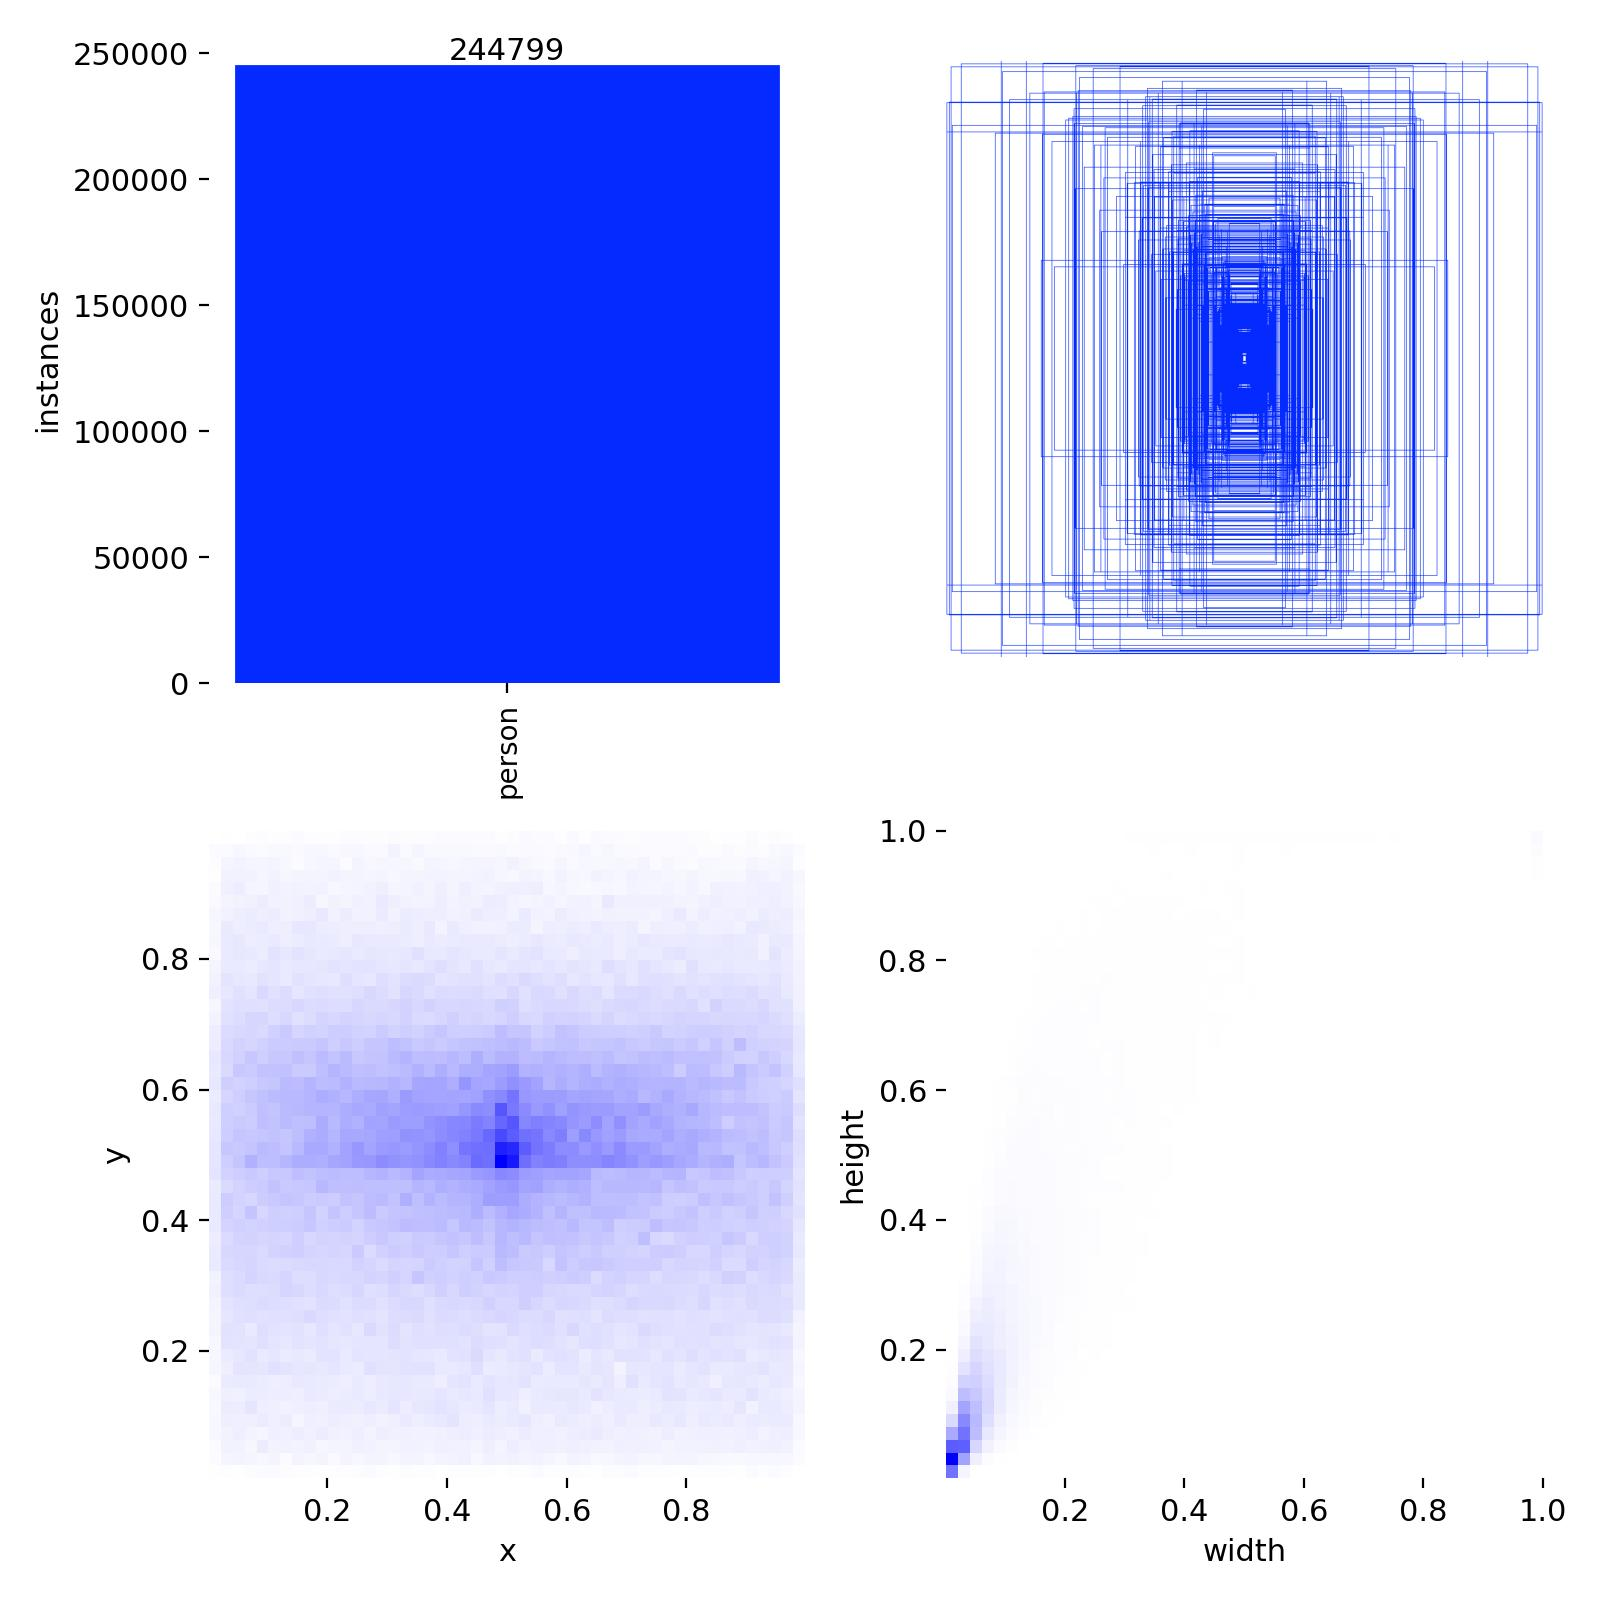
\includegraphics[width=0.6\linewidth]{bab4/labels}
	\caption{Visualisasi distribusi label dan persebaran \textit{bounding box} dataset person-only}
	\label{fig:labels_distribution}
\end{figure}

Berdasarkan hasil pemeriksaan dataset, total data citra yang digunakan pada proses pelatihan dan validasi berjumlah 123.287 gambar dengan total 116.497 file anotasi.
Distribusi \textit{bounding box} menunjukkan bahwa mayoritas objek manusia berada pada area tengah citra dengan variasi ukuran kecil hingga menengah.
Hal ini sesuai dengan karakteristik dataset umum COCO yang banyak berisi objek manusia dalam skenario aktivitas sehari-hari.


\subsection{Analisis Proses Training Model}

Proses konvergensi selama pelatihan model dipantau secara berkala melalui evaluasi nilai \textit{loss} dan peningkatan metrik akurasi pada setiap \textit{epoch}. Grafik perkembangan parameter pelatihan dan validasi tersebut digambarkan pada Gambar \ref{fig:training_results}.

\begin{figure}[H]
	\centering
	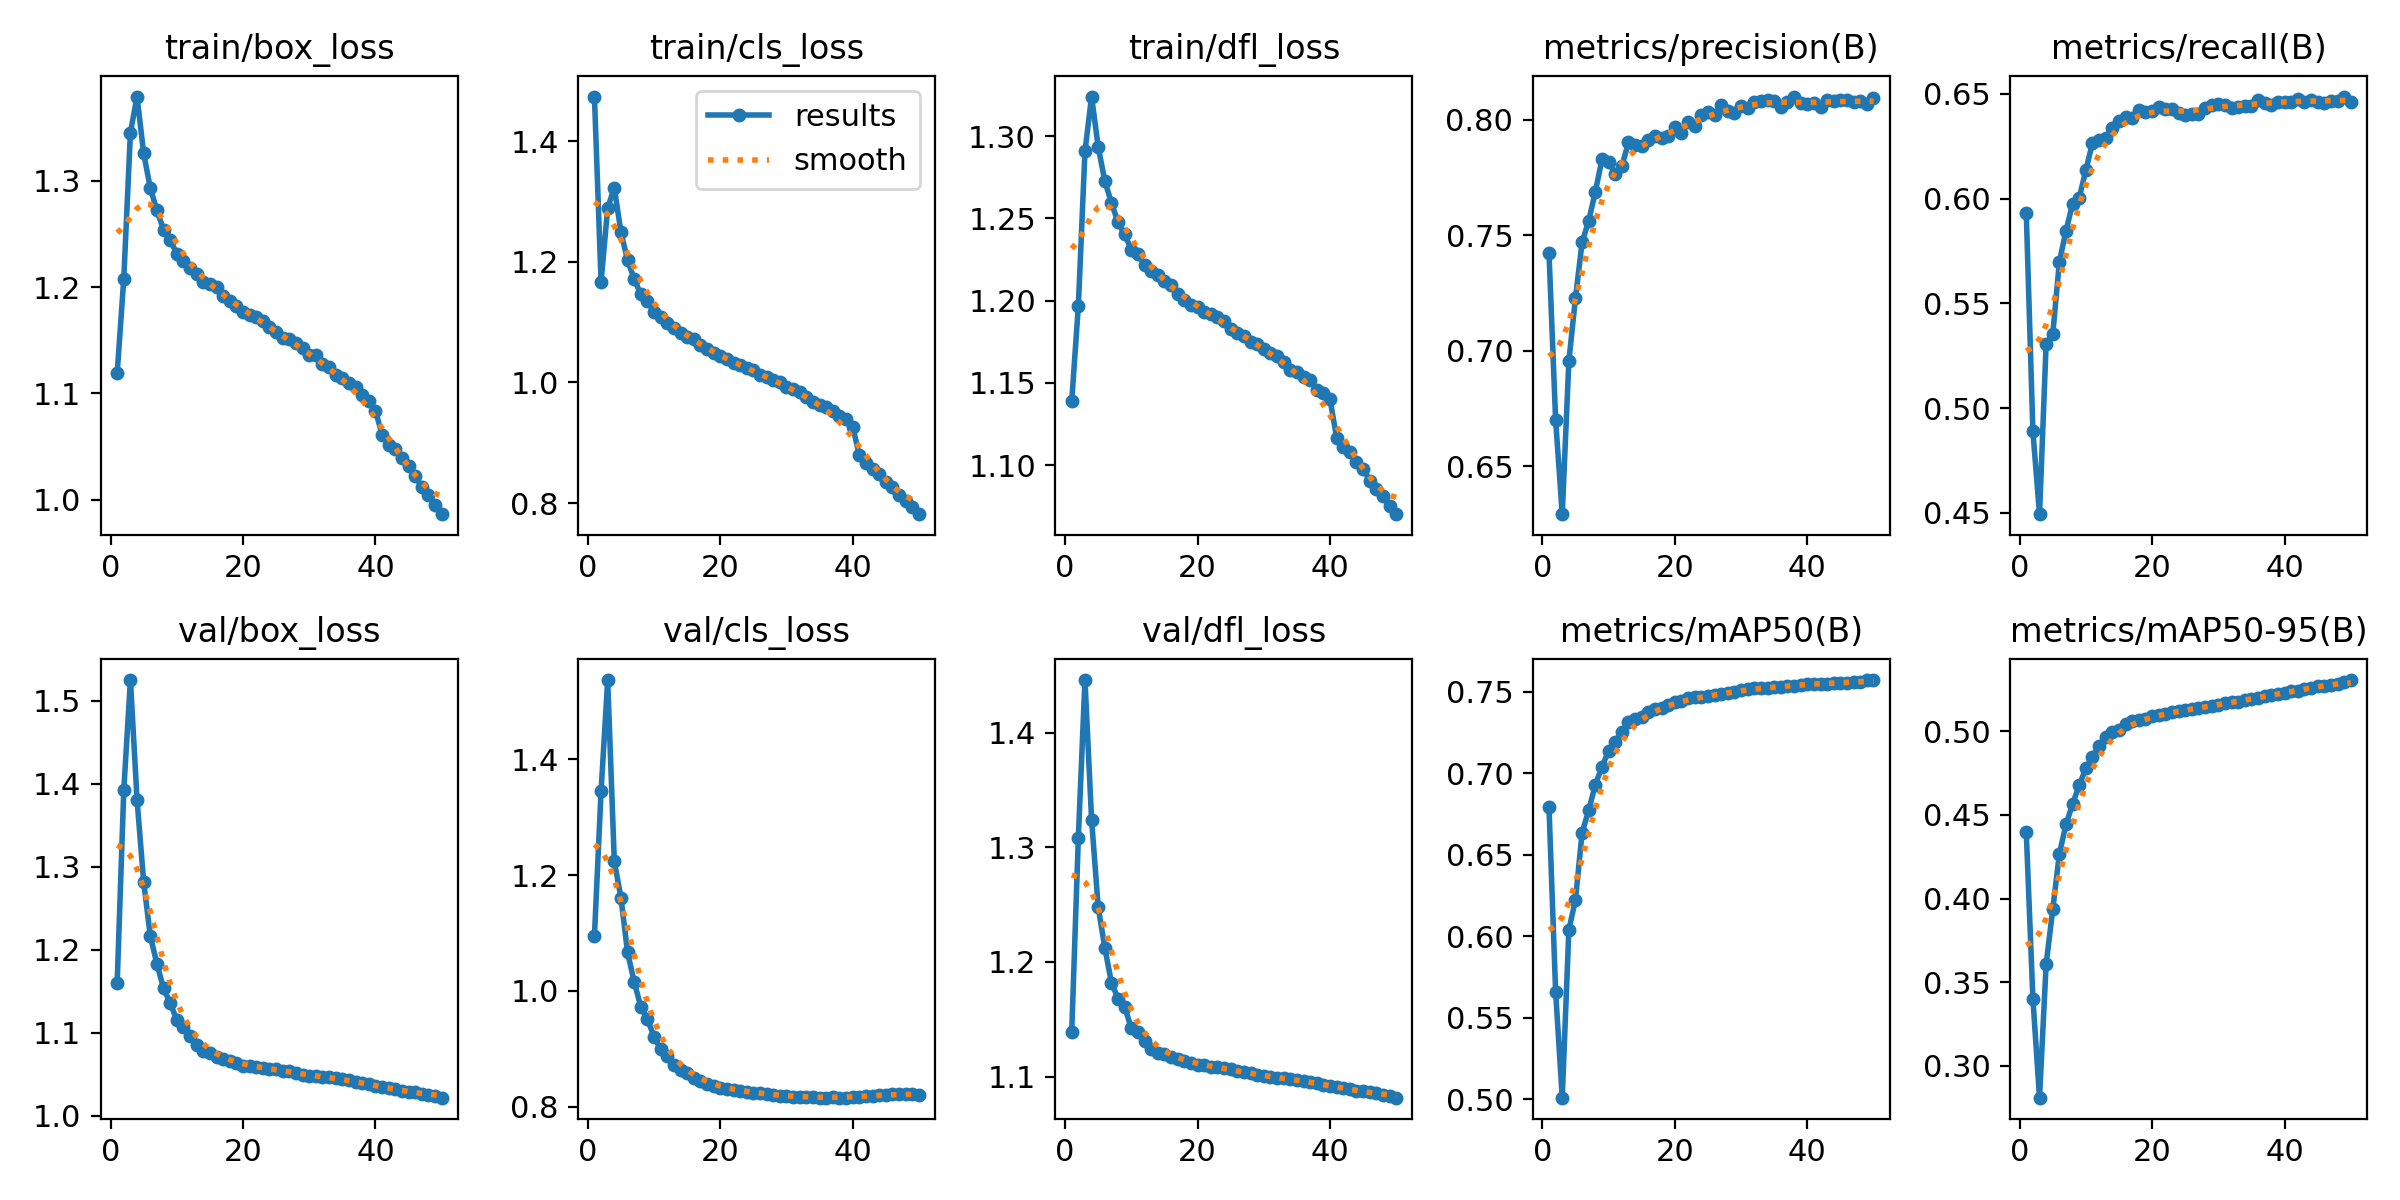
\includegraphics[width=\linewidth]{bab4/results}
	\caption{Grafik perkembangan training loss, validation loss, precision, recall, dan mAP}
	\label{fig:training_results}
\end{figure}

Seluruh komponen loss mengalami penurunan stabil selama proses training. Box loss pelatihan turun dari 1,1189 ke 0,9864, sementara class loss pelatihan berkurang signifikan dari 1,4740 menjadi 0,7816 pada epoch akhir. Pada saat yang sama, metrics precision (B) meningkat secara bertahap hingga mencapai 0,8092, recall (B) mencapai 0,6463, dan metrik mAP@50 mencapai 0,7572 pada epoch 50. Penurunan \textit{train loss} dan \textit{validation loss} yang relatif konsisten menunjukkan bahwa proses pelatihan berjalan stabil tanpa divergensi signifikan. Selain itu, tidak terlihat peningkatan \textit{validation loss} secara ekstrem pada epoch akhir (di mana box loss validasi stabil pada 1,0219 dan class loss validasi stabil pada 0,8208) sehingga indikasi overfitting berat tidak ditemukan pada model hasil \textit{fine-tuning}.

Melalui perolehan grafik evaluasi training yang menunjukkan kestabilan nilai \textit{loss} serta peningkatan nilai mAP yang konvergen, model deteksi YOLOv8n ini dinilai telah matang dan siap diintegrasikan. Kestabilan kurva performa tersebut memberikan jaminan bahwa model tidak mengalami gejala \textit{overfitting} maupun \textit{underfitting} selama proses pembelajaran berlangsung. Dengan ukuran bobot model yang kompak hasil pemangkasan kelas target, model ini memiliki kesiapan optimal untuk dieksekusi pada lingkungan komputasi terbatas di dalam \textit{companion computer} Raspberry Pi 5. Oleh karena itu, bobot model final ini dapat langsung dideploy untuk mendukung proses inferensi visual secara \textit{real-time} pada sistem navigasi otonom.

\subsection{Hasil Evaluasi Model}

Setelah pelatihan selesai, performa model YOLOv8n hasil \textit{fine-tuning} dievaluasi dengan dataset pengujian terpisah. Rincian metrik evaluasi akhir model disajikan pada Tabel \ref{tab:metric_result}.

\begin{table}[H]
	\centering
	\caption{Hasil Evaluasi Akhir Model YOLOv8n}
	\label{tab:metric_result}
	\renewcommand{\arraystretch}{1.2}
	\begin{tabular}{|l|c|}
		\hline
		Metrik & Nilai \\ \hline
		
		Precision & 0.809 \\ \hline
		Recall & 0.646 \\ \hline
		mAP@50 & 0.757 \\ \hline
		mAP@50-95 & 0.531 \\ \hline
		F1-Score & 0.720 \\ \hline
		Threshold Optimal & 0.224 \\ \hline
	\end{tabular}
\end{table}

Nilai precision yang tinggi menunjukkan bahwa model mampu meminimalkan false positive, sedangkan nilai recall menunjukkan masih terdapat beberapa objek manusia kecil yang belum terdeteksi secara optimal.

Nilai metrik evaluasi yang disajikan pada Tabel~\ref{tab:metric_result} memiliki dampak langsung terhadap efisiensi eksekusi secara \textit{real-time} pada Raspberry Pi 5. Keandalan komputasi dalam menghasilkan nilai latensi rendah dan \textit{frame rate} (FPS) tinggi pada unit \textit{companion computer} sangat dipengaruhi oleh tingkat kompleksitas arsitektur jaringan saraf tiruan yang digunakan. Melalui penyederhanaan arsitektur model YOLOv8n kelas tunggal dan pembatasan resolusi input sebesar 320x320 piksel, beban pemrosesan dapat diredam secara signifikan tanpa mengorbankan akurasi secara drastis. Dengan demikian, optimasi parameter arsitektur model ini menjadi prasyarat krusial agar sirkuit asinkron pendeteksi target mampu bersinkronisasi secara tepat dengan frekuensi kontrol otonom.

\subsection{Analisis Precision, Recall, dan F1-Score}

Untuk mengevaluasi performa deteksi model secara lebih rinci, dilakukan analisis terhadap hubungan confidence threshold dengan F1-score dan Precision-Recall sebagaimana ditunjukkan pada Gambar \ref{fig:boxf1_curve} dan Gambar \ref{fig:boxpr_curve}.

\begin{figure}[H]
	\centering
	\begin{minipage}{0.48\linewidth}
		\centering
		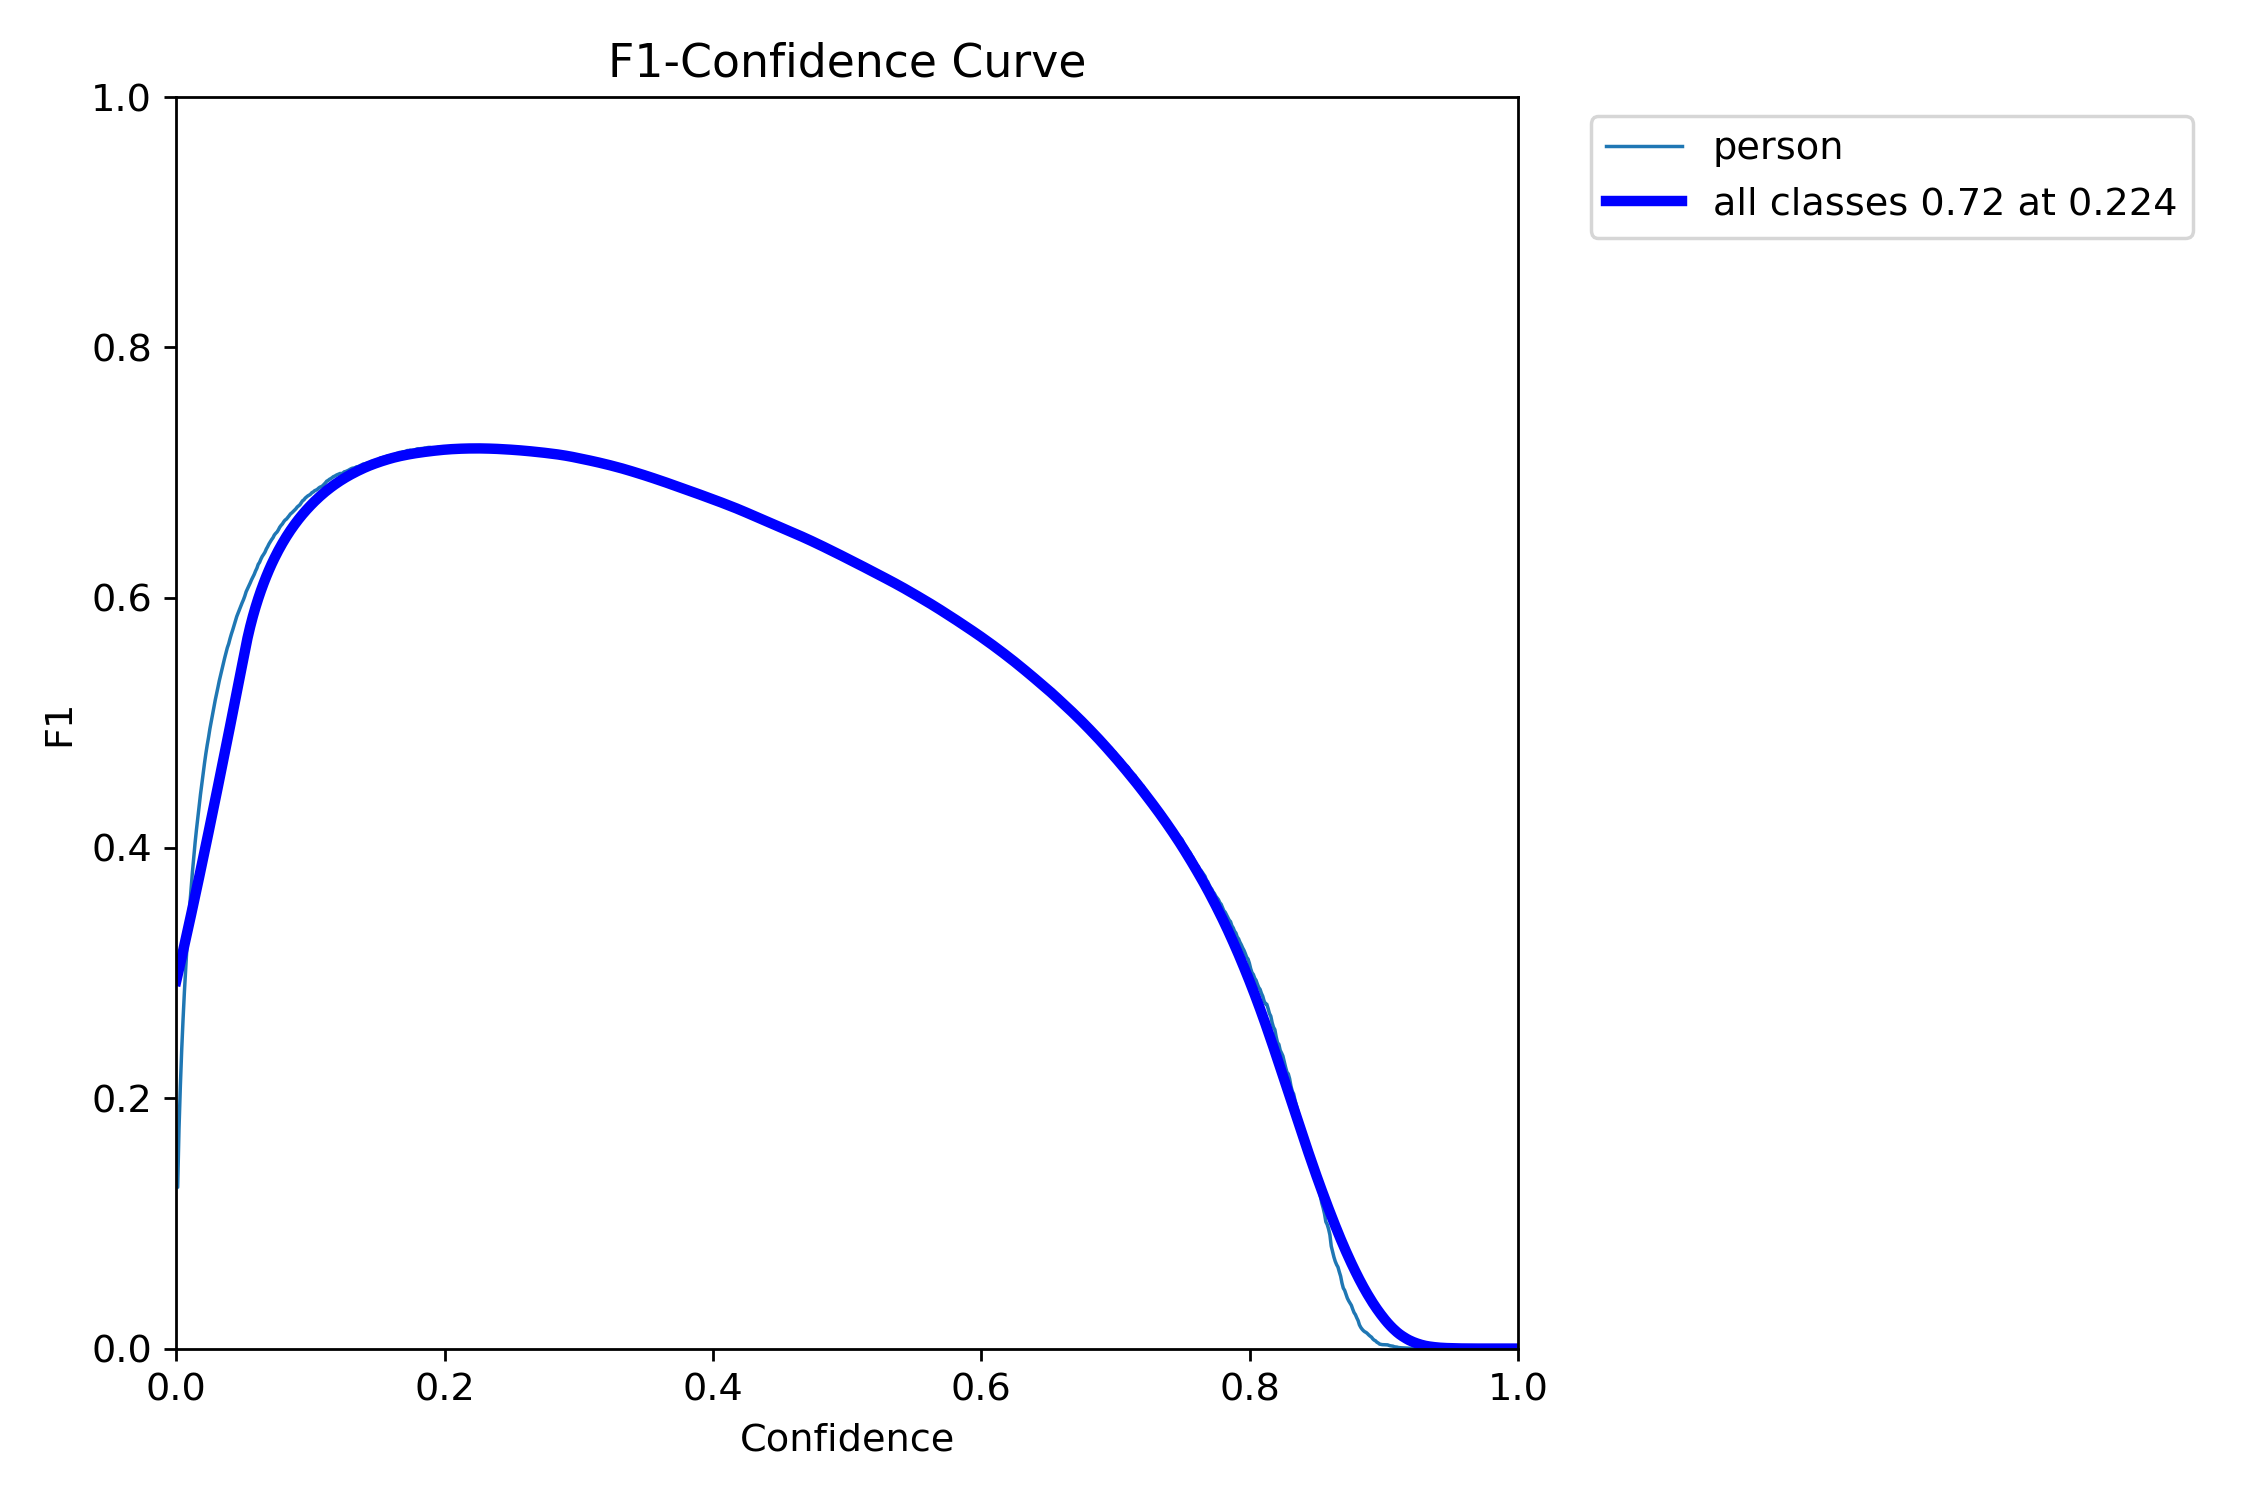
\includegraphics[width=\linewidth]{bab4/BoxF1_curve}
		\caption{Kurva F1-Confidence model YOLOv8n}
		\label{fig:boxf1_curve}
	\end{minipage}
	\hfill
	\begin{minipage}{0.48\linewidth}
		\centering
		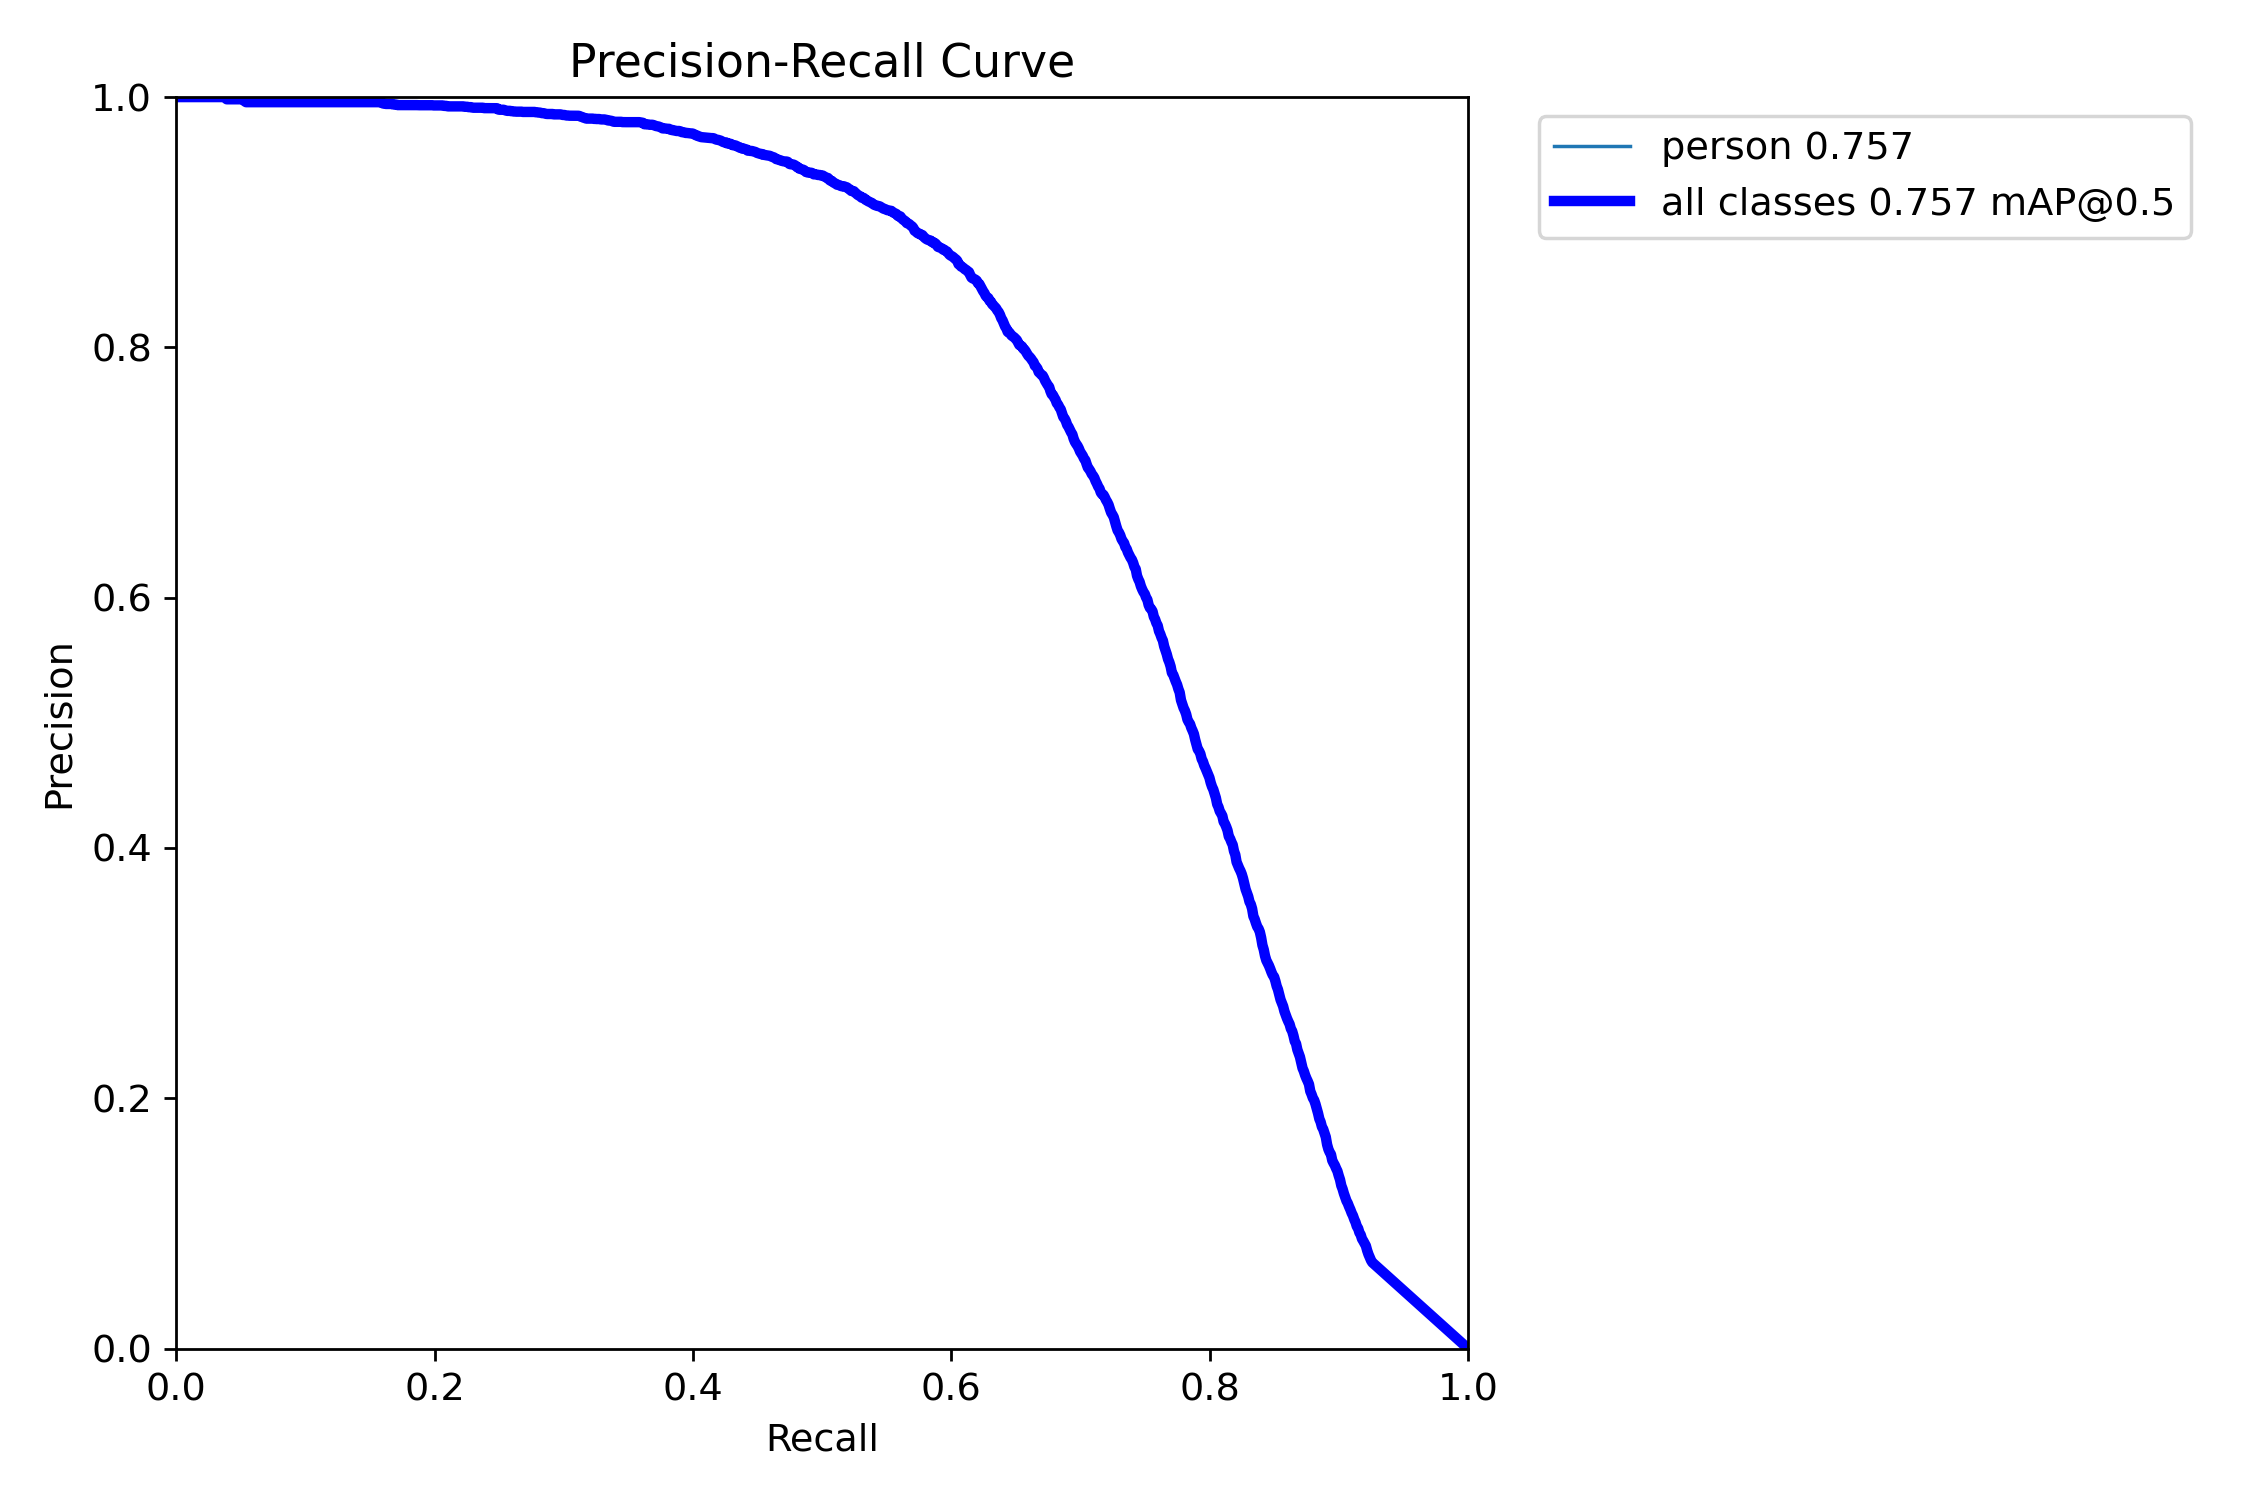
\includegraphics[width=\linewidth]{bab4/BoxPR_curve}
		\caption{Kurva Precision-Recall model YOLOv8n}
		\label{fig:boxpr_curve}
	\end{minipage}
\end{figure}

Berdasarkan hasil pengujian, peningkatan confidence threshold menyebabkan precision meningkat namun recall menurun.
Hal ini menunjukkan adanya tradeoff antara sensitivitas deteksi dan minimisasi false positive.
Kurva F1-score menunjukkan nilai optimum diperoleh pada confidence threshold sekitar 0.224 dengan nilai F1-score maksimum sekitar 0.72.
Threshold tersebut kemudian digunakan sebagai konfigurasi inferensi utama pada sistem drone otonom.
Kurva Precision-Recall menunjukkan bahwa model masih mampu mempertahankan tingkat precision yang relatif tinggi sebelum recall mencapai nilai maksimum.
Hal ini menunjukkan bahwa model cukup efektif dalam mengurangi false positive pada sebagian besar kondisi pengujian.

\subsection{Analisis Confusion Matrix}

Untuk memetakan distribusi klasifikasi benar dan kesalahan deteksi model secara spesifik, matriks kebingungan (\textit{confusion matrix}) diekstraksi dari hasil validasi. Distribusi persentase klasifikasi tersebut divisualisasikan pada Gambar \ref{fig:conf_matrix_norm}.

\begin{figure}[H]
	\centering
	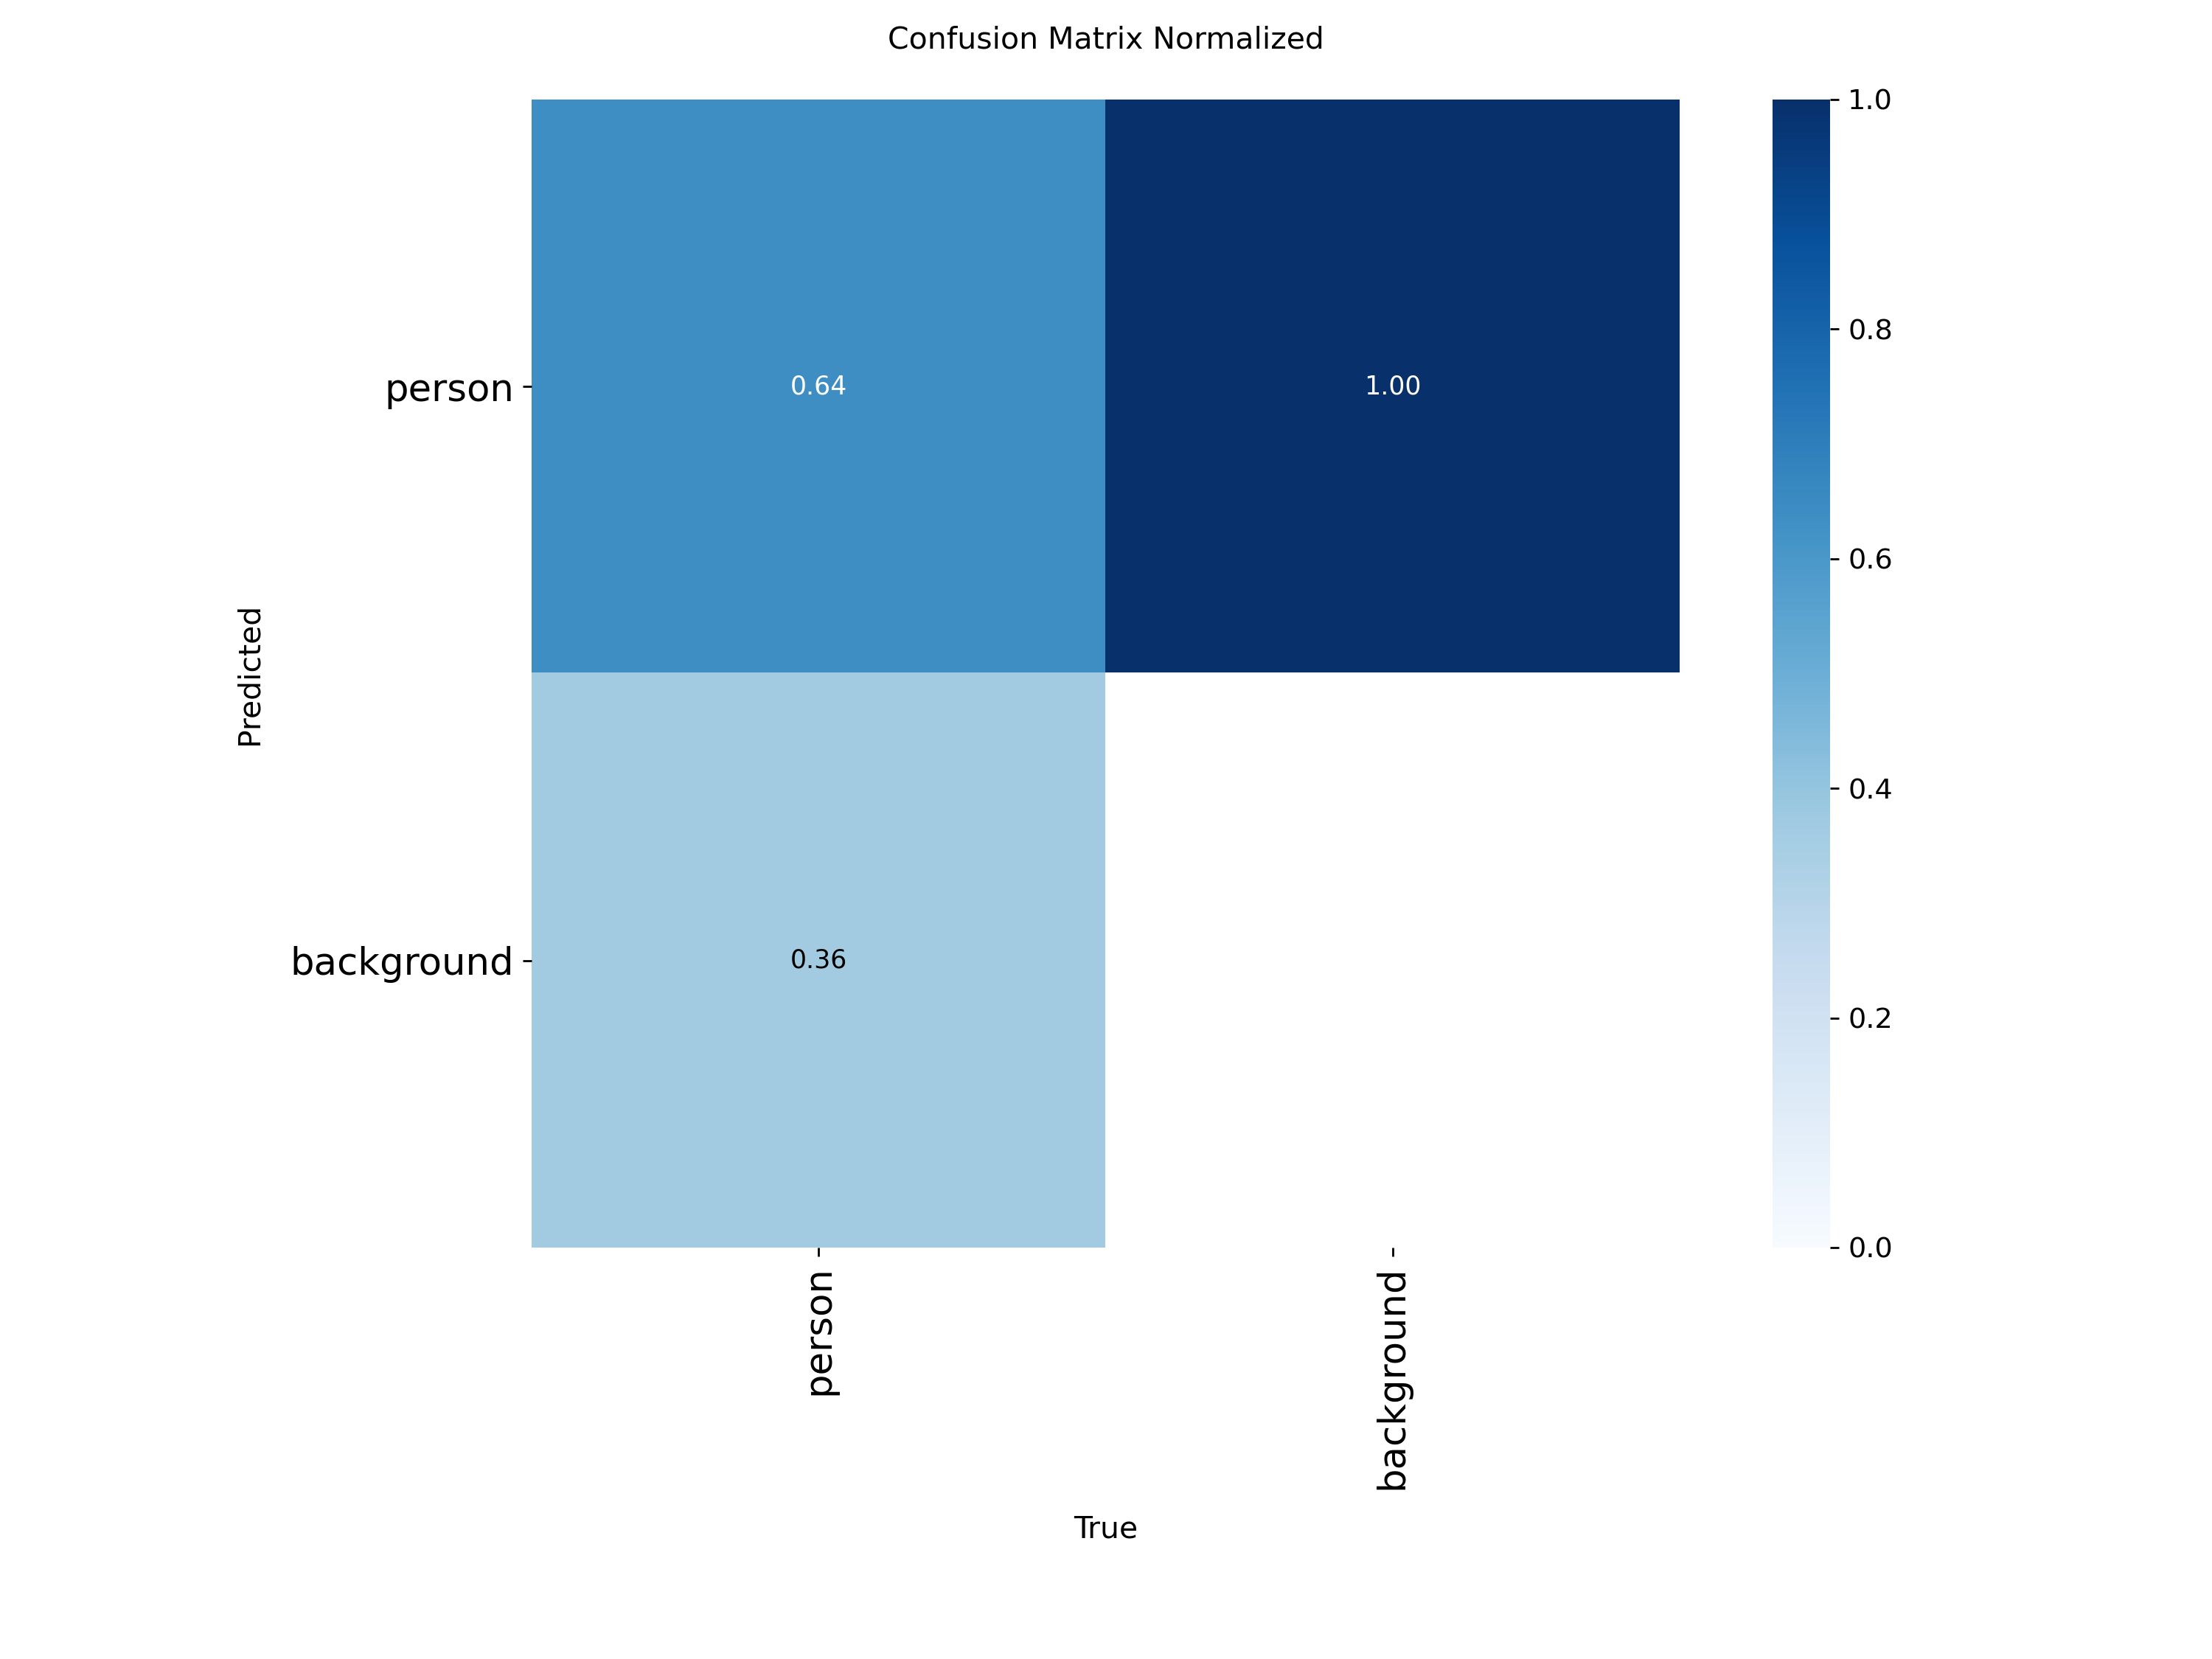
\includegraphics[width=0.6\linewidth]{bab4/confusion_matrix_normalized}
	\caption{Normalized confusion matrix}
	\label{fig:conf_matrix_norm}
\end{figure}

Berdasarkan Gambar \ref{fig:conf_matrix_norm}, model YOLOv8n hasil \textit{fine-tuning} mencatat tingkat \textit{True Positive} (manusia terdeteksi sebagai manusia) sebesar 65\%. Tingkat \textit{False Negative} (tidak terdeteksi) tercatat sebesar 35\%, dipengaruhi oleh target kecil atau terhalang vegetasi. Kesalahan klasifikasi latar belakang sebagai manusia (\textit{False Positive}) bernilai sangat rendah, membuktikan keandalan model dalam membedakan target dari objek lingkungan.

\subsection{Analisis Hasil Prediksi Validasi}

Untuk mengevaluasi kualitas deteksi model, dilakukan perbandingan antara ground truth dataset dan hasil prediksi model pada batch validasi sebagaimana ditunjukkan pada Gambar \ref{fig:val_compare0}. Visualisasi ini menyandingkan label anotasi asli dengan kotak pembatas prediktif beserta tingkat kepercayaannya. Perbandingan visual ini penting untuk mengamati kemampuan model dalam menangani variasi bentuk tubuh manusia secara spasial.

\begin{figure}[H]
	\centering
	
	\begin{minipage}{0.48\linewidth}
		\centering
		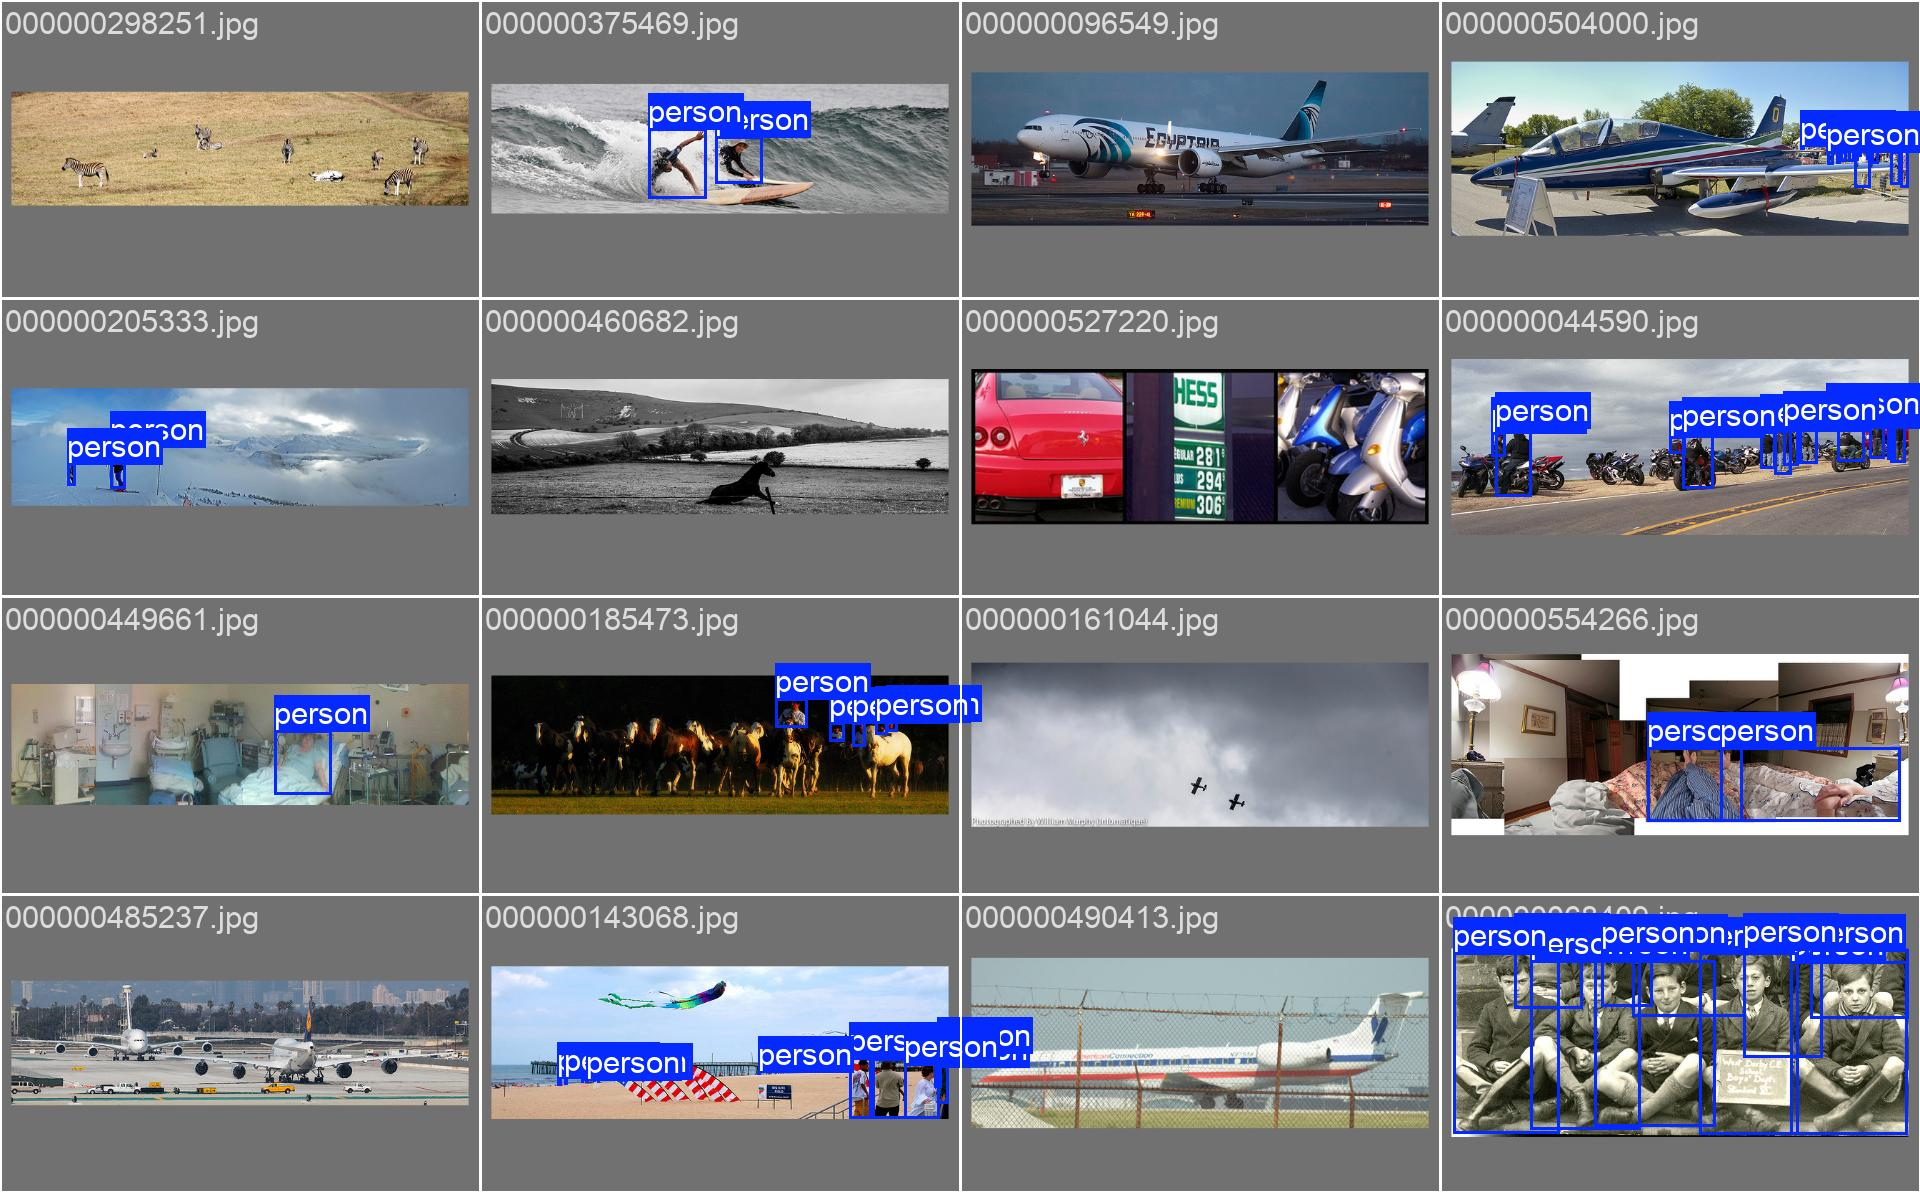
\includegraphics[width=\linewidth]{bab4/val_batch0_labels}
		\small (a) Ground truth batch validasi ke-0
	\end{minipage}
	\hfill
	\begin{minipage}{0.48\linewidth}
		\centering
		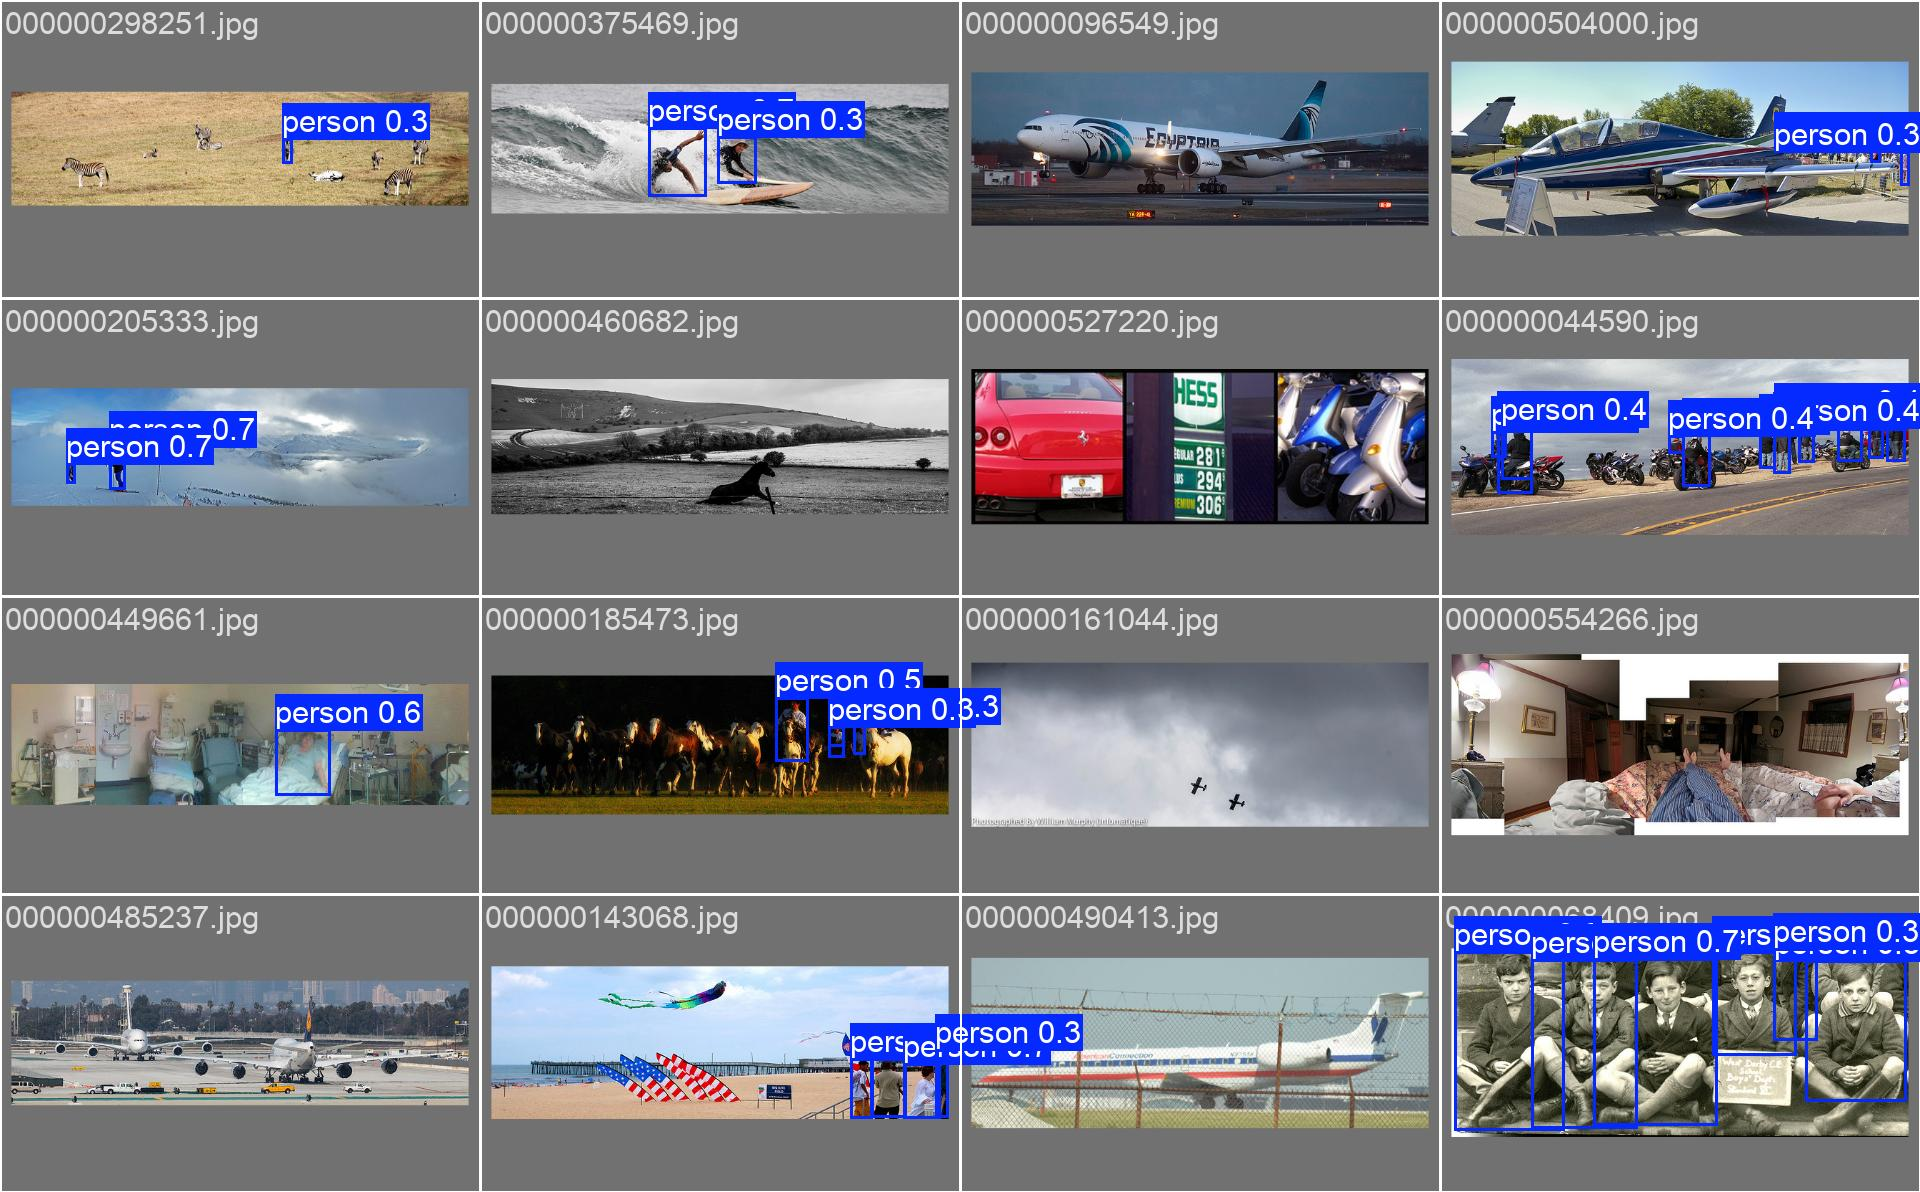
\includegraphics[width=\linewidth]{bab4/val_batch0_pred}
		\small (b) Hasil prediksi model batch validasi ke-0
	\end{minipage}
	
	\caption{Perbandingan ground truth dan hasil prediksi pada batch validasi ke-0}
	\label{fig:val_compare0}
\end{figure}

Hasil validasi menunjukkan bahwa model masih mampu mendeteksi manusia pada kondisi keramaian, variasi pose tubuh, dan sebagian objek dengan ukuran relatif kecil.
Namun demikian, confidence deteksi cenderung menurun pada objek yang mengalami occlusion atau berada jauh dari kamera.
Perbandingan antara ground truth dan hasil prediksi menunjukkan bahwa model berhasil mengikuti mayoritas \textit{bounding box} manusia, sejalan dengan perolehan nilai mAP@50 sebesar 0,757 pada pengujian sebelumnya.
Selain itu, model juga mampu mempertahankan konsistensi deteksi pada beberapa kondisi lingkungan kompleks dengan banyak objek manusia dalam satu citra.
\subsection{Perbandingan Resolusi Inferensi Model Hasil \textit{Fine-Tuning}}

Setelah memperoleh model terbaik dari proses \textit{fine-tuning}, penelitian ini mengevaluasi pengaruh resolusi inferensi terhadap performa komputasi pada Raspberry Pi 5. Pengujian ini dilakukan menggunakan model YOLOv8n hasil \textit{fine-tuning} yang telah diekspor ke format ONNX Runtime dengan variasi resolusi input 256×256, 320×320, dan 640×640 sebagaimana ditunjukkan pada Tabel \ref{tab:benchmark_resolution}.

\begin{table}[H]
	\centering
	\caption{Perbandingan Resolusi Inferensi YOLOv8n Hasil Fine-Tuning pada Raspberry Pi 5}
	\label{tab:benchmark_resolution}
	\renewcommand{\arraystretch}{1.2}
	\begin{tabular}{|p{2.5cm}|p{2cm}|p{3cm}|p{2cm}|p{3cm}|}
		\hline
		\textbf{Model} &
		\textbf{Input} &
		\textbf{Output Shape} &
		\textbf{FPS} &
		\textbf{Inferensi (ms)} \\ \hline
		
		256n &
		256 &
		[1, 84, 1344] &
		35.54 &
		28.13 \\ \hline
		
		320n &
		320 &
		[1, 84, 2100] &
		23.72 &
		42.17 \\ \hline
		
		640n &
		640 &
		[1, 84, 8400] &
		5.84 &
		171.22 \\ \hline
	\end{tabular}
\end{table}

Hasil pengujian menunjukkan bahwa peningkatan resolusi inferensi menyebabkan latensi meningkat secara signifikan akibat bertambahnya kompleksitas komputasi pada proses inferensi model. Karakteristik grafik perbandingan performa dari variasi resolusi ini diperjelas pada Gambar \ref{fig:onnx_compare}.

\begin{figure}[H]
	\centering
	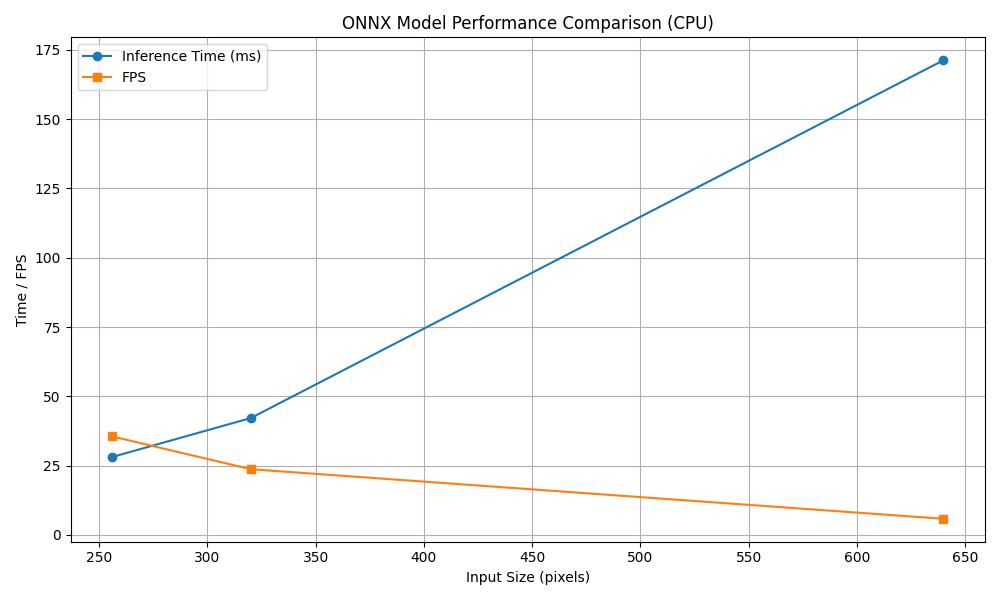
\includegraphics[width=0.9\linewidth]{bab4/onnx_performance_comparison}
	\caption{Perbandingan performa model ONNX hasil fine-tuning pada Raspberry Pi 5}
	\label{fig:onnx_compare}
\end{figure}

Berdasarkan hasil benchmark tersebut, peningkatan resolusi input memberikan pengaruh yang signifikan terhadap korelasi antara kecepatan sistem dan detail spasial citra. Model dengan resolusi 256×256 menghasilkan performa inferensi tercepat dengan rata-rata latensi sekitar 28,13 ms dan FPS mencapai sekitar 35,54 FPS. Namun demikian, pada beberapa kondisi outdoor ditemukan penurunan kualitas deteksi manusia berukuran kecil akibat detail spasial citra yang lebih rendah.

Sebaliknya, resolusi 640×640 menghasilkan kualitas visual yang lebih baik namun menyebabkan beban komputasi pada CPU meningkat tajam sehingga latensi membengkak hingga sekitar 171,22 ms dan performa menurun signifikan hingga hanya mencapai sekitar 5,84 FPS. Kondisi ini dinilai tidak memenuhi kebutuhan sistem navigasi drone otonom \textit{real-time} karena delay inferensi terlalu tinggi untuk proses pengambilan keputusan secara langsung.

Resolusi 320×320 menghasilkan kompromi terbaik antara performa \textit{real-time} dan kualitas deteksi objek manusia. Dengan rata-rata latensi sekitar 42,17 ms dan FPS sekitar 23,72 FPS, sistem masih mampu mempertahankan operasi \textit{real-time} sambil menghasilkan \textit{bounding box} yang stabil. Selain itu, resolusi ini juga memberikan hasil deteksi yang lebih baik pada kondisi lingkungan kompleks dengan variasi pencahayaan dan ukuran objek manusia yang beragam. Berdasarkan hasil pengujian komparatif tersebut, resolusi 320×320 dipilih sebagai konfigurasi inferensi final yang diimplementasikan pada platform \textit{edge computing} drone otonom secara \textit{real-time}.

Justifikasi pemilihan resolusi 320x320 piksel ini juga didasarkan pada aspek pengelolaan termal dan efisiensi sumber daya komputasi Raspberry Pi 5. Penggunaan resolusi yang lebih rendah dari 640x640 piksel mampu menekan utilisasi CPU dan RAM tetap berada pada batas aman, sehingga mencegah terjadinya peningkatan suhu berlebih (\textit{thermal throttling}) pada sirkuit \textit{edge computing}. Melalui efisiensi beban kerja tersebut, sistem otonom drone dapat mempertahankan latensi end-to-end yang rendah secara konstan selama misi berlangsung. Dengan demikian, konfigurasi ini tidak hanya menjaga stabilitas performa sistem tetapi juga mendukung respons navigasi otonom yang aman dan andal.

Hasil perbandingan performa inferensi dan parameter komputasi tersebut selanjutnya diintegrasikan ke dalam subsistem utama pendukung. Sinergi antarmuka komputasi edge ini akan dievaluasi secara terintegrasi dengan modul telemetri dan kendali otonom pada tahapan pengujian berikutnya.

\section{Pengujian Integrasi Sistem Backend, MAVSDK, dan Frontend}

Pengujian ini dilakukan untuk memastikan seluruh arsitektur perangkat lunak mampu berjalan secara bersamaan tanpa saling memblokir (blocking) pada Raspberry Pi 5 selama operasi drone berlangsung. Fokus utama diarahkan pada sinkronisasi pembagian memori antar-thread untuk menghindari race condition. Melalui sinergi antar-proses ini, keandalan fungsional dari seluruh arsitektur asinkron backend-frontend dapat dipastikan aman sebelum uji terbang otonom.

\subsection{Pengujian Integrasi Backend dan Multi-Threading}

Pengujian integrasi memverifikasi arsitektur \textit{multi-threading} pada skrip \texttt{app.py} berjalan tanpa hambatan. Log Flask dan SocketIO (Gambar \ref{fig:logflask1} dan Gambar \ref{fig:logflask2}) menunjukkan server aktif di port 3000. Utas \texttt{YOLOConsumer} (Gambar \ref{fig:logyolo}) memproses antrean citra GStreamer (Gambar \ref{fig:loggstreamer}) secara paralel, sementara kestabilan inferensi (\textit{inference\_ms}) terjaga tanpa memblokir pembaruan telemetri utas \texttt{MAVSDKListener}.

\begin{figure}[H]
	\centering
	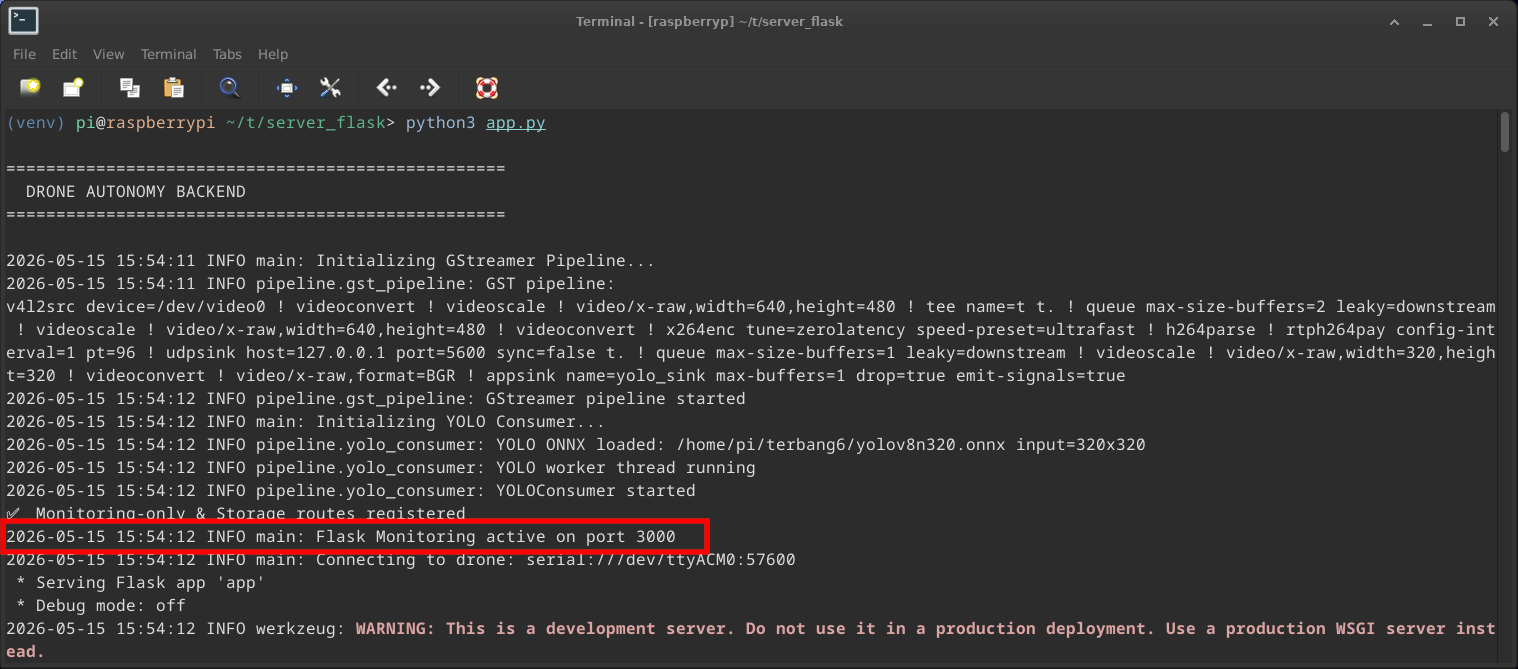
\includegraphics[width=\textwidth]{bab4/screenshot_flask_log} 
	\caption{Log aktivitas server Flask dan SocketIO}
	\label{fig:logflask1}
	
	\vspace{0.5cm}
	
	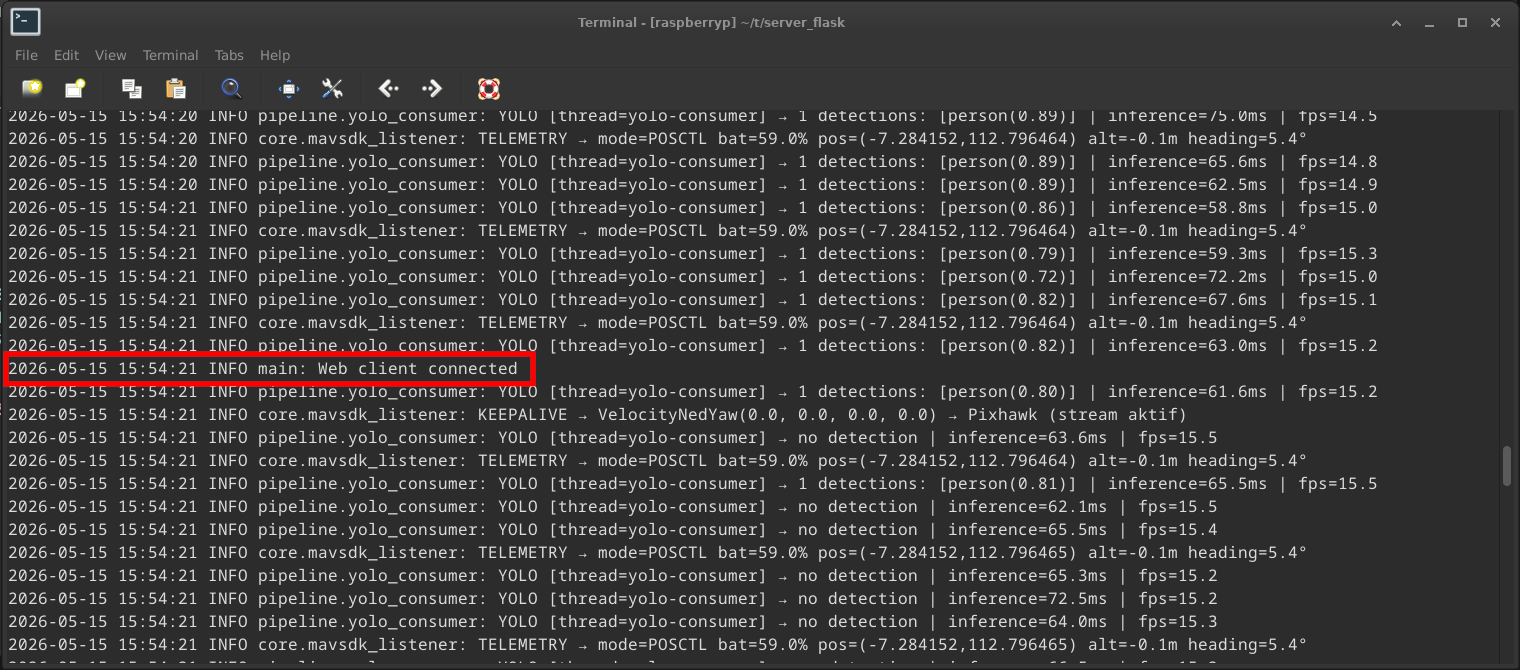
\includegraphics[width=\textwidth]{bab4/screenshot_flask_log_2} 
	\caption{Log aktivitas server Flask dan SocketIO 2}
	\label{fig:logflask2}
\end{figure}

\begin{figure}[H]
	\centering
	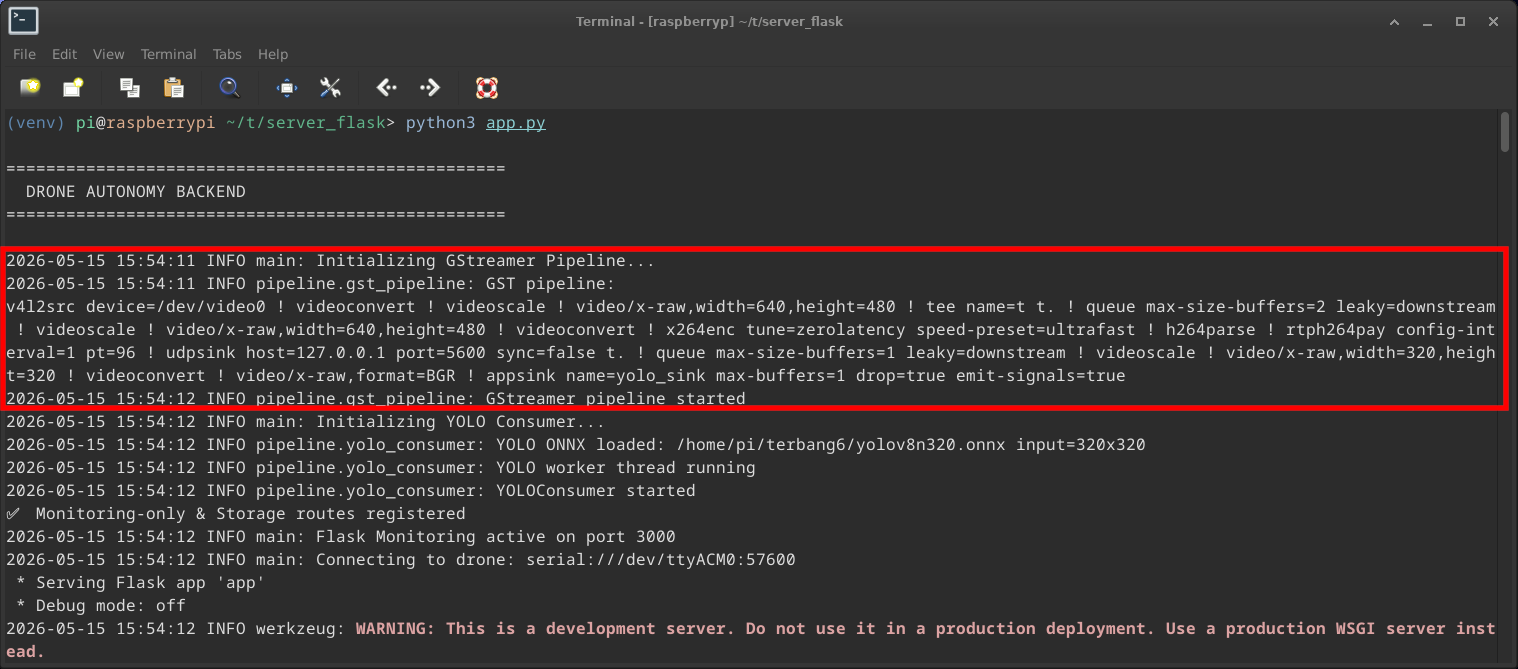
\includegraphics[width=\textwidth]{bab4/diagram_gstreamer_pipeline} 
	\caption{Implementasi percabangan aliran video GStreamer}
	\label{fig:loggstreamer}
	
	\vspace{0.5cm}
	
	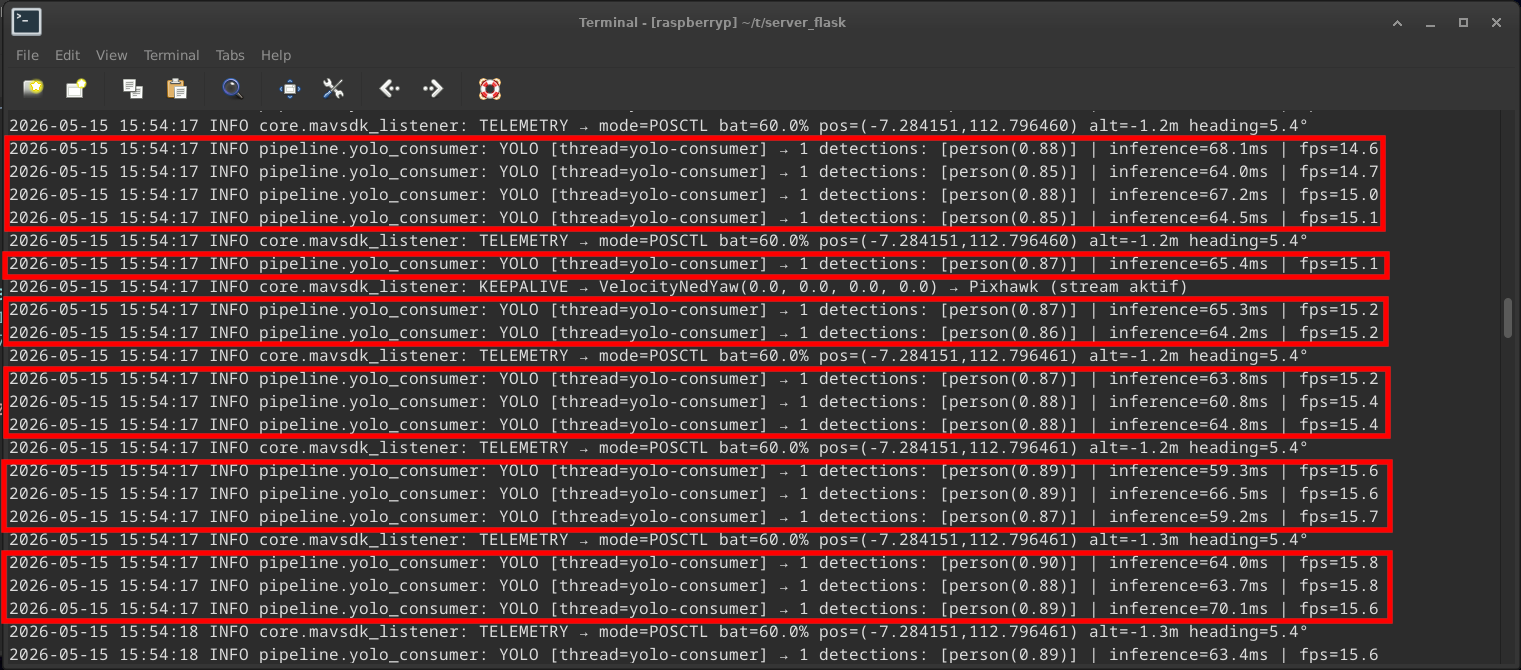
\includegraphics[width=\textwidth]{bab4/screenshot_yolo_inference} 
	\caption{Eksekusi deteksi objek YOLOv8 pada \textit{thread} terpisah}
	\label{fig:logyolo}
\end{figure}

Integrasi pemrosesan video dan inferensi YOLOv8n pada Gambar \ref{fig:loggstreamer} dan Gambar \ref{fig:logyolo} terbukti berjalan secara paralel tanpa hambatan pada antrean data. Penjadwalan \textit{thread} terpisah memungkinkan penanganan visual berjalan dengan waktu inferensi yang stabil di dalam batas toleransi \textit{real-time}, sehingga siap dihubungkan dengan modul telemetri drone.

\subsection{Pengujian Aliran Telemetri MAVSDK ke Frontend}

Validasi komunikasi asinkron dilakukan dengan mengamati aliran data dari pengontrol terbang ke dasbor web. Melalui log terminal Gambar \ref{fig:logtelemmavsdk}, kelas \texttt{MAVSDKListener} membaca status penerbangan (seperti mode, baterai, ketinggian, dan kecepatan) lewat \textit{event loop} \texttt{asyncio}, lalu memancarkannya via \textit{event} \texttt{drone:status}. Keberhasilan transmisi dikonfirmasi pada dasbor operator (Gambar \ref{fig:logsocket}), di mana antarmuka React menerima muatan JSON setiap interval 200 ms (5 Hz) menggunakan modul \texttt{socket.js}.

\begin{figure}[H]
	\centering
	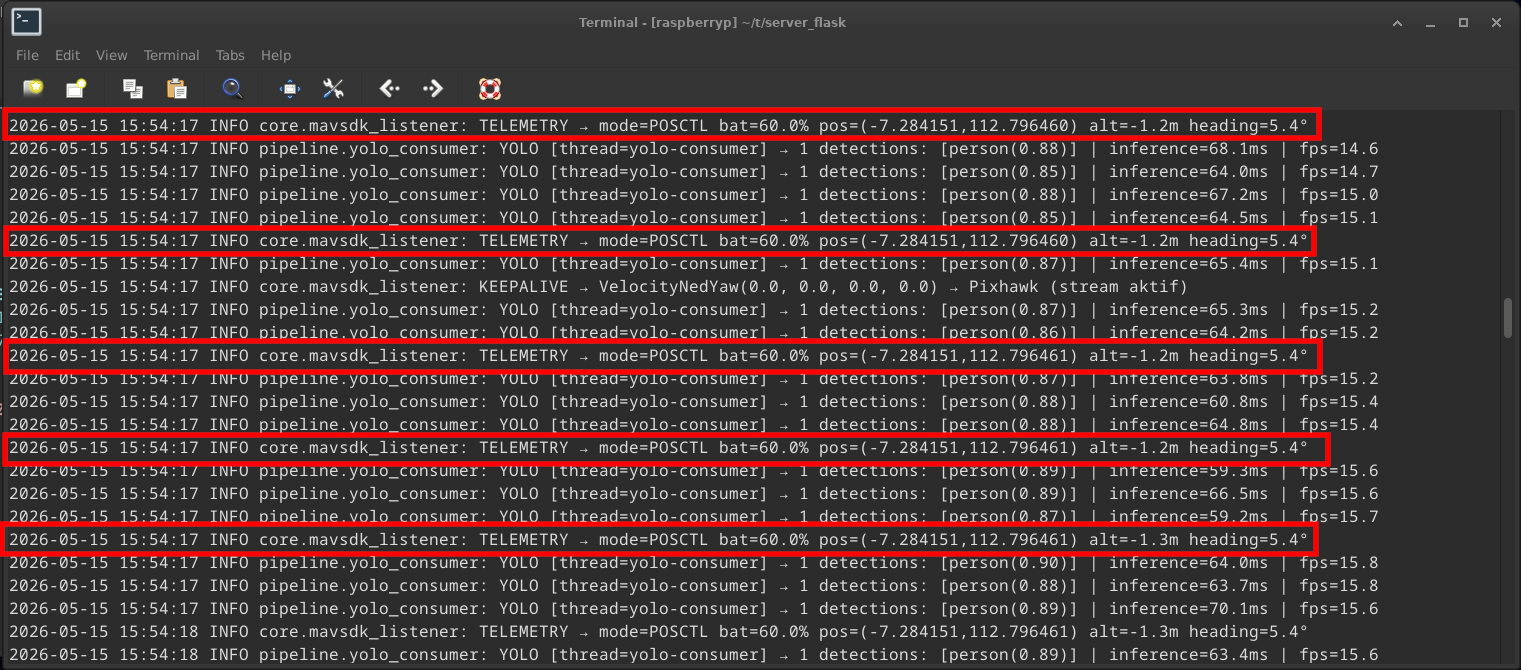
\includegraphics[width=\textwidth]{bab4/screenshot_mavsdk_stream} 
	\caption{Proses \textit{streaming} telemetri melalui MAVSDK}
	\label{fig:logtelemmavsdk}
	
	\vspace{0.5cm}
	
	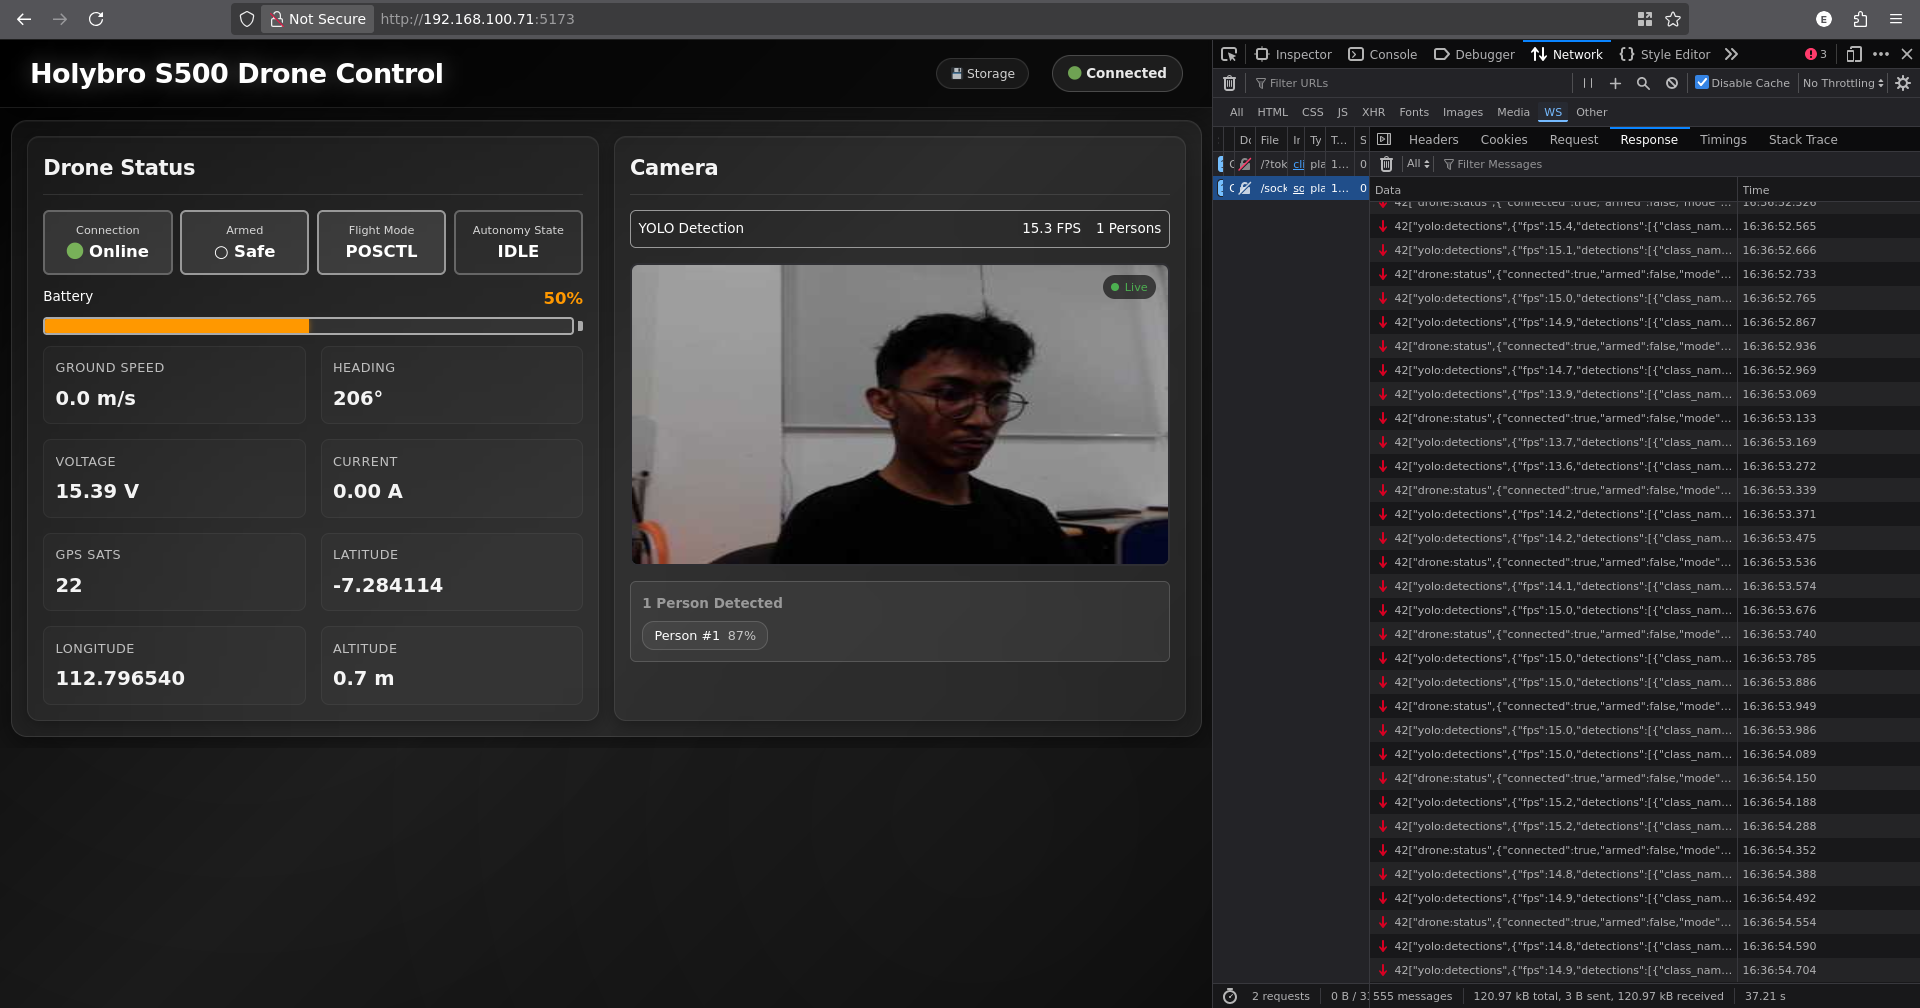
\includegraphics[width=\textwidth]{bab4/screenshot_socket_update} 
	\caption{Visualisasi pembaruan data \textit{real-time} pada antarmuka}
	\label{fig:logsocket}
\end{figure}

Kelancaran transmisi telemetri nirkabel dari flight controller ke dasbor operator divalidasi oleh log terminal pada Gambar \ref{fig:logtelemmavsdk} dan Gambar \ref{fig:logsocket}. Protokol SocketIO berhasil memperbarui status terbang secara berkala tanpa ada kehilangan paket data (\textit{packet loss}) dengan tingkat latensi minimal, yang membuktikan kesiapan modul backend untuk dihubungkan ke antarmuka pengguna.

\subsection{Pengujian Fungsional Antarmuka Dashboard}

Pengujian fungsional \textit{dashboard} dilakukan untuk memvalidasi performa antarmuka berbasis React dalam merender data secara \textit{real-time}. Pada Gambar \ref{fig:uiweb1} dan Gambar \ref{fig:uiweb2}, komponen \texttt{DroneStatus.jsx} berhasil memvisualisasikan seluruh metrik absolut drone dengan latensi yang minimal. Komponen \texttt{VideoControl.jsx} juga berhasil merender kotak pembatas (\textit{bounding box}) target secara dinamis beserta nilai \textit{confidence} dari algoritma YOLOv8. Sistem pelaporan keadaan (\textit{state machine}) juga berjalan sesuai skenario \textit{Scout Mission}, di mana status transisi dari \texttt{SCAN} menuju \texttt{APPROACH} dan \texttt{DOCUMENT} terpantau langsung oleh operator.

\begin{figure}[H]
	\centering
	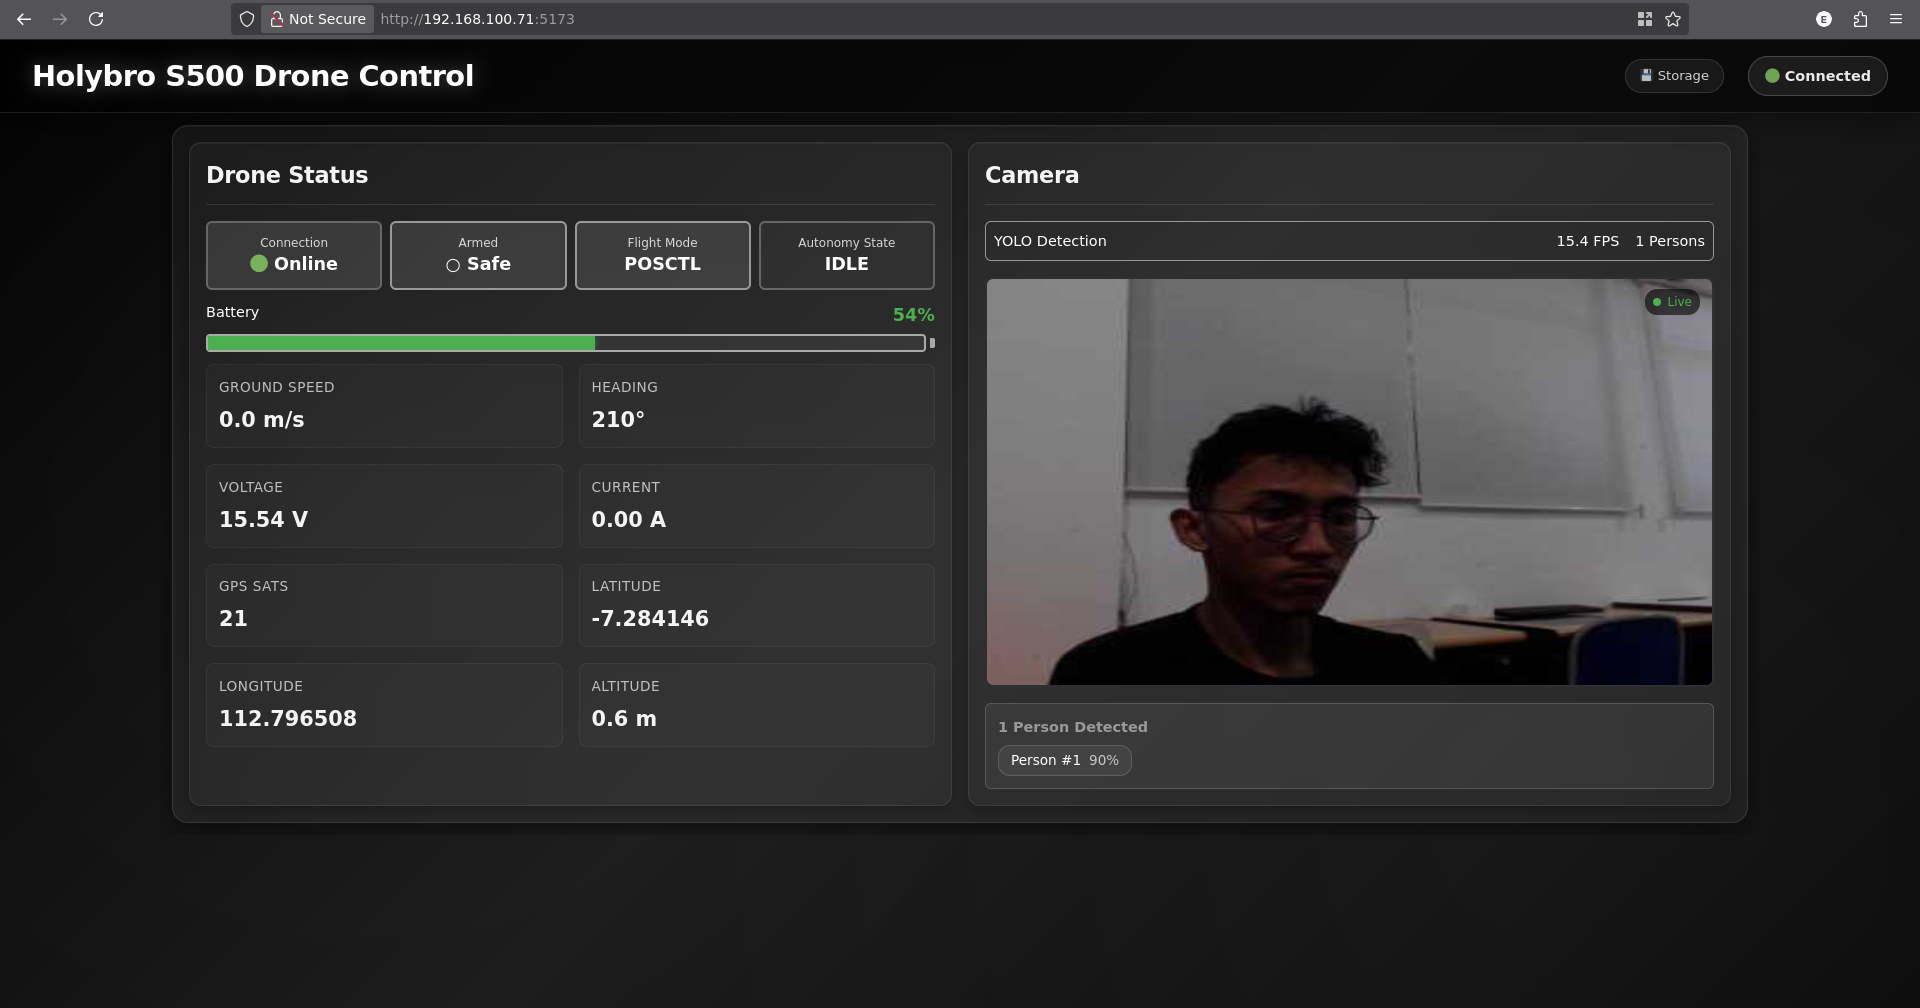
\includegraphics[width=\textwidth]{bab4/screenshot_ui_dashboard} 
	\caption{Tampilan antarmuka dashboard monitoring operator 1}
	\label{fig:uiweb1}
	
	\vspace{0.5cm}
	
	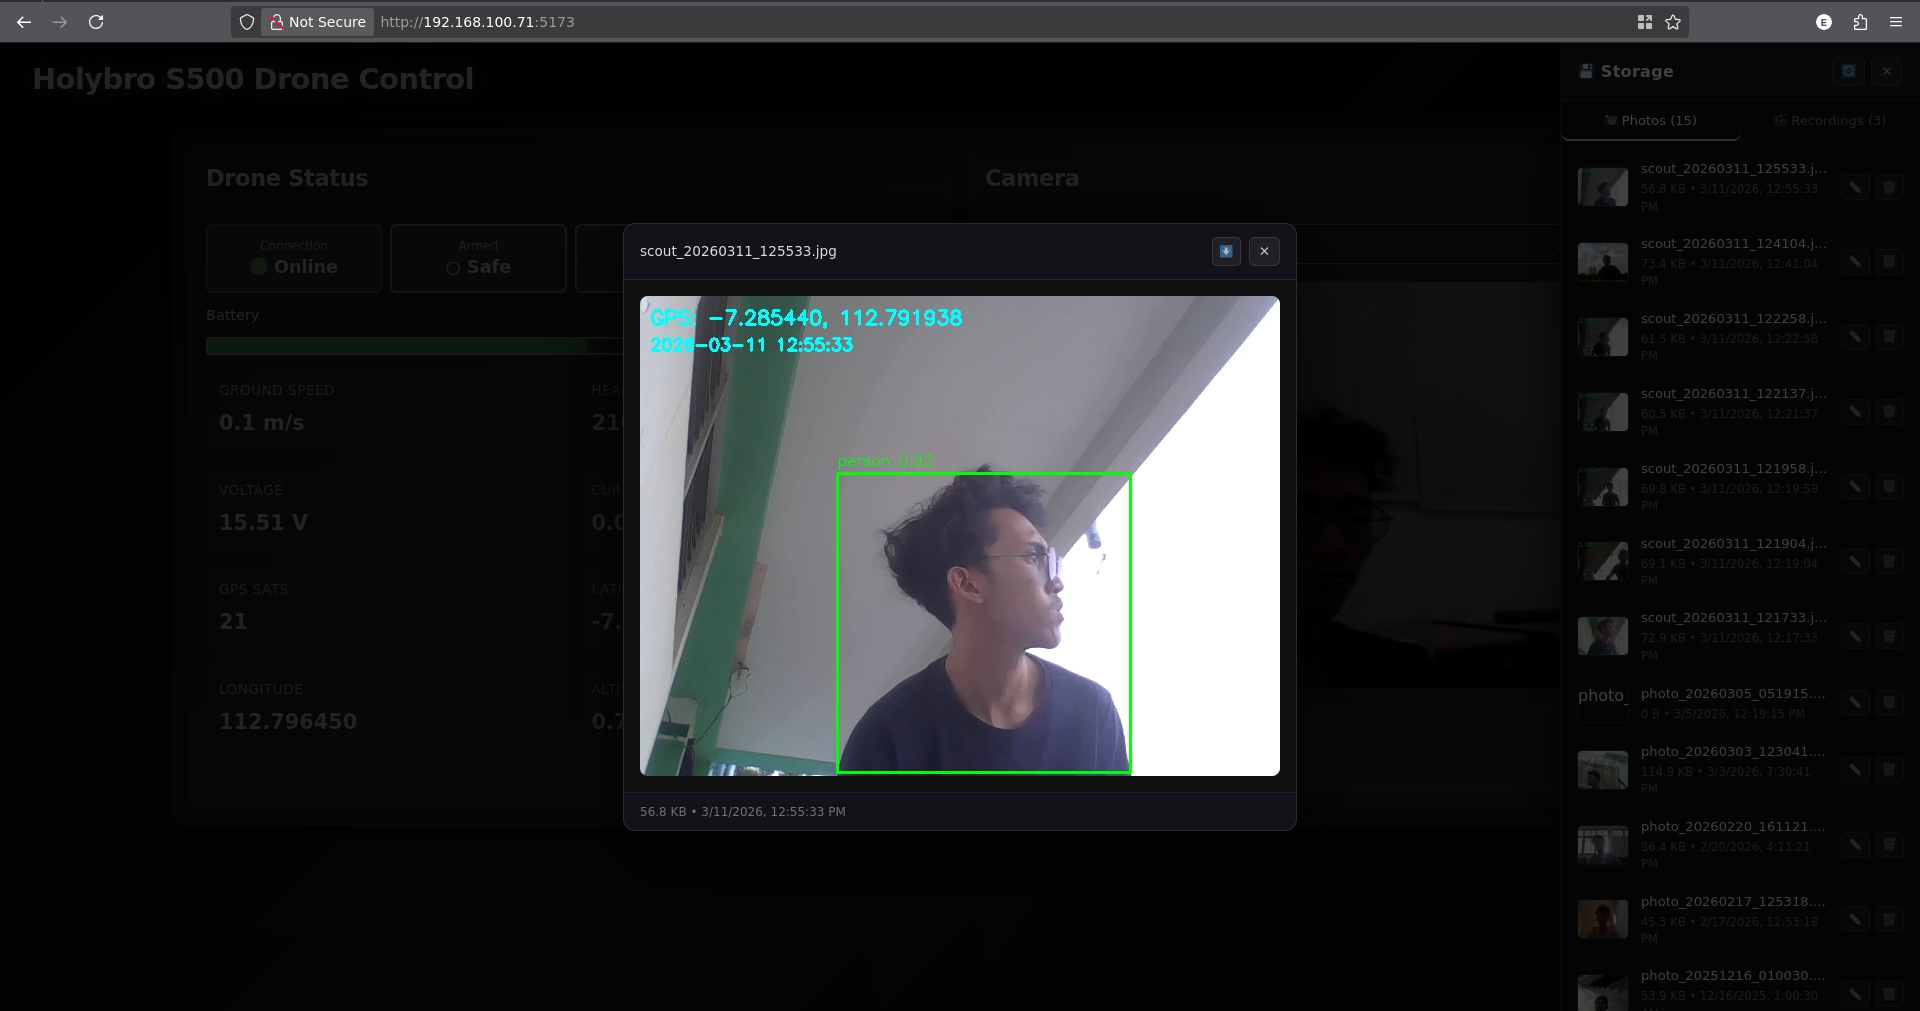
\includegraphics[width=\textwidth]{bab4/screenshot_ui_dashboard_2} 
	\caption{Tampilan antarmuka dashboard monitoring operator 2}
	\label{fig:uiweb2}
\end{figure}

Visualisasi dasbor React 19 pada Gambar \ref{fig:uiweb1} dan Gambar \ref{fig:uiweb2} menunjukkan rendering aliran video dan status drone yang dinamis. Responsivitas antarmuka tetap terjaga selama drone melakukan manuver otonom kompleks, sehingga memvalidasi kesiapan sistem untuk pengujian di bawah variasi kualitas jaringan nirkabel.

\subsection{Evaluasi Stabilitas Jaringan MiFi 4G/5G dan Transmisi Video}

Selain pengujian fungsionalitas antarmuka, penelitian ini juga mengevaluasi keandalan transmisi data menggunakan koneksi MiFi 4G/5G \textit{onboard} sebagai jalur komunikasi nirkabel antara drone dan laptop operator (\textit{Ground Control Station}). Hasil pengujian menunjukkan bahwa pengiriman matriks data telemetri JSON (melalui WebSockets) maupun transmisi video latensi rendah (melalui protokol UDP) berjalan stabil dengan frekuensi pembaruan 5 Hz selama kedua perangkat beroperasi di lapangan terbuka dengan visibilitas langsung (\textit{Line-of-Sight} / LoS).

Namun demikian, ketika lintasan sinyal seluler terhalang oleh struktur fisik seperti area pepohonan atau dinding bangunan luar ruang, antarmuka pemantauan web mulai mengalami degradasi performa. Masalah ini paling terlihat pada aliran video UDP yang seketika mengalami penumpukan \textit{frame} (\textit{stuttering} atau patah-patah) hingga \textit{freeze} di pihak peramban operator akibat redaman sinyal. Menariknya, meskipun antarmuka pengawasan mengalami \textit{lag} visual yang cukup parah, rekaman \textit{log} di dalam drone membuktikan bahwa pemrosesan inferensi YOLOv8n, eksekusi \textit{state machine} otonom, dan pergerakan aktual drone (\textit{edge processing}) sama sekali tidak terganggu dan tetap berjalan mulus. Fenomena ini mengonfirmasi bahwa arsitektur \textit{edge computing} berhasil mengamankan stabilitas komputasi kritis di atas drone secara independen tanpa bergantung pada \textit{bandwidth} jaringan, memvalidasi bahwa isu patah-patah visual murni merupakan limitasi daya pancar gelombang seluler dalam menembus rintangan ruang.

Hasil evaluasi fungsional dari seluruh komponen di atas drone menjadi dasar untuk pengujian keandalan sistem secara terintegrasi. Selanjutnya, performa drone otonom divalidasi secara komparatif melalui serangkaian skenario uji terbang nyata di lapangan.

\section{Validasi Integrasi Sistem Drone Otonom}

Pengujian akhir dilakukan pada skenario operasi drone otonom secara menyeluruh. Tahap penutupan pengujian ini bertujuan untuk memvalidasi performa terintegrasi dari seluruh modul yang telah dikembangkan secara parsial. Melalui skenario misi terpadu di lapangan terbuka, keandalan platform dalam mengeksekusi misi pencarian korban secara utuh dapat diukur secara kuantitatif.

\subsection{Metodologi dan Pemetaan Sesi Penerbangan}

Validasi integrasi sistem drone otonom secara menyeluruh dirancang ke dalam sembilan skenario pengujian spesifik (Skenario A hingga I) yang mencakup evaluasi \textit{state machine}, akurasi deteksi, navigasi, performa komputasi, hingga keselamatan terbang. Untuk mencapai efisiensi operasional dan menghemat alokasi baterai, keseluruhan skenario pengujian tersebut diimplementasikan secara komprehensif dan dipetakan ke dalam lima sesi penerbangan nyata (Flight~1 hingga Flight~5). 

Pemetaan skenario pengujian terhadap sesi penerbangan nyata dirangkum pada Tabel \ref{tab:pemetaan_skenario}. Setiap skenario diberi kode alfabet A hingga I untuk memudahkan kategorisasi. Distribusi sesi penerbangan ini disesuaikan dengan kapasitas daya baterai serta prioritas evaluasi di lapangan.

\begin{table}[H]
	\centering
	\caption{Pemetaan Skenario Pengujian terhadap Sesi Penerbangan Nyata}
	\label{tab:pemetaan_skenario}
	\renewcommand{\arraystretch}{1.2}
	\begin{tabular}{|c|p{7cm}|p{4cm}|}
		\hline
		\textbf{Kode} & \textbf{Fokus Skenario Pengujian} & \textbf{Sesi Penerbangan} \\ \hline
		A & Pengujian Validasi State Machine (FSM) Scout & Flight~1, Flight~2 \\ \hline
		B & Pengujian Akurasi Deteksi In-Flight & Flight~3 \\ \hline
		C & Pengujian Latensi Pipeline End-to-End & Flight~1 \\ \hline
		D & Pengujian Akurasi Navigasi Otonom & Flight~1, Flight~2 \\ \hline
		E & Pengujian Respons Safety Override dan Safety System & Flight~1, Flight~2 \\ \hline
		F & Pengujian Persistent Multi-Target Scouting & Flight~1, Flight~2, Flight~5 \\ \hline
		G & Pengujian Target Lock Stability \& EMA Smoothing & Flight~4 \\ \hline
		H & Pengujian Performa Termal dan Resource & Flight~4 \\ \hline
		I & Pengujian Kondisi Lingkungan Bervariasi & Flight~3 \\ \hline
	\end{tabular}
\end{table}

Pemetaan skenario pada Tabel \ref{tab:pemetaan_skenario} dirancang untuk memaksimalkan efisiensi pengujian lapangan dengan menggabungkan beberapa target evaluasi ke dalam satu sesi penerbangan tunggal. Integrasi beberapa skenario uji dalam satu penerbangan ini penting untuk mereplikasi kompleksitas misi pencarian riil di mana deteksi, keputusan navigasi, dan protokol keselamatan berjalan secara simultan di bawah batasan kapasitas baterai yang terbatas.

Kondisi operasional dan hasil observasi umum dari kelima sesi penerbangan tersebut dirangkum pada Tabel \ref{tab:skenario_validasi}. Rangkuman ini mencakup jumlah target yang diidentifikasi, intervensi pengendali jarak jauh (RC Override), serta pemicu keselamatan baterai otomatis. Log observasi ini menjadi basis data kuantitatif utama untuk mengevaluasi keandalan misi di lapangan.

\begin{table}[H]
	\centering
	\caption{Kondisi Operasional dan Rangkuman Sesi Penerbangan Nyata}
	\label{tab:skenario_validasi}
	\renewcommand{\arraystretch}{1.2}
	\begin{tabular}{|p{1.5cm}|p{4cm}|p{7cm}|}
		\hline
		\textbf{Flight} & \textbf{Kondisi Operasional} & \textbf{Hasil Observasi Umum} \\ \hline
		
		Flight~1 &
		Scout mission lengkap tanpa intervensi &
		10 siklus SCAN$\to$APPROACH$\to$DOCUMENT$\to$
		DISPLACING berhasil penuh; battery RTL otomatis terpicu pada 13\% \\ \hline
		
		Flight~2 &
		Scout mission panjang dengan RC Override &
		5 target terdokumentasi; RC Override (POSCTL) terjadi beberapa kali; battery RTL terpicu pada 14\% \\ \hline
		
		Flight~3 &
		Pengujian deteksi manusia multi-jarak &
		Deteksi diuji pada jarak 5, 10, 15, dan 20~m; diulang di dua lokasi berbeda \\ \hline
		
		Flight~4 &
		Target acquisition dengan dua orang &
		Dua manusia terdeteksi dalam satu frame secara bersamaan; \textit{lock\_init} berhasil; RC Override terjadi \\ \hline
		
		Flight~5 &
		Scout mission tambahan &
		Siklus SCAN$\to$DOCUMENT terkonfirmasi; RC Override terjadi beberapa kali \\ \hline
	\end{tabular}
\end{table}

Data operasional penerbangan yang terangkum dalam Tabel~\ref{tab:skenario_validasi} menjadi basis empiris untuk memvalidasi performa sistem otonom pada Skenario A hingga F. Setiap baris data dalam tabel tersebut merepresentasikan eksekusi sekuensial misi pencarian korban secara otonom yang dimulai sejak fase lepas landas (\textit{takeoff}) hingga pendaratan (\textit{landing}). Dari pencatatan penerbangan nyata ini, interaksi dinamis antara model deteksi dan pengambil keputusan dapat dievaluasi secara komprehensif pada berbagai skenario uji. Dengan demikian, rekam jejak operasional dari kelima penerbangan tersebut memberikan bukti konkret mengenai keandalan integrasi sistem dalam kondisi lingkungan dinamis di lapangan.

\subsection{Skenario A: Pengujian Validasi State Machine (FSM) Scout Mission}

Validasi transisi \textit{Finite State Machine} (FSM) dilakukan berdasarkan data log dari lima sesi penerbangan (Flight~1 hingga Flight~5). Pengujian bertujuan untuk memverifikasi bahwa seluruh transisi state yang dirancang pada Bab~3 dapat dieksekusi sesuai urutan operasi misi, serta mengevaluasi kemampuan sistem dalam menangani kondisi kegagalan selama proses pencarian dan pendekatan target.

Berdasarkan analisis log, seluruh transisi utama FSM berhasil dieksekusi sesuai urutan yang diharapkan, yaitu SCAN $\rightarrow$ APPROACH $\rightarrow$ DOCUMENT $\rightarrow$ DISPLACING $\rightarrow$ SCAN. Selain itu, sistem juga berhasil menjalankan mekanisme \textit{failback} APPROACH $\rightarrow$ SCAN ketika target hilang dari bidang pandang kamera (\textit{target lost}). Rekapitulasi hasil pengujian ditunjukkan pada Tabel \ref{tab:fsm_transitions}.

\begin{table}[H]
	\centering
	\caption{Hasil Pengujian Validasi State Machine (FSM) Scout Mission}
	\label{tab:fsm_transitions}
	\renewcommand{\arraystretch}{1.2}
	\begin{tabular}{|l|c|c|c|c|}
		\hline
		\textbf{Transisi} & \textbf{Percobaan} & \textbf{Berhasil} & \textbf{Gagal} & \textbf{Success Rate (\%)} \\ \hline
		SCAN $\to$ APPROACH & 38 & 38 & 0 & 100.0\% \\ \hline
		APPROACH $\to$ DOCUMENT & 38 & 30 & 8 & 78.9\% \\ \hline
		DOCUMENT $\to$ DISPLACING & 30 & 30 & 0 & 100.0\% \\ \hline
		DISPLACING $\to$ SCAN & 29 & 29 & 0 & 100.0\% \\ \hline
		APPROACH $\to$ SCAN (\textit{timeout}) & 0 & 0 & 0 & 0.0\% \\ \hline
		APPROACH $\to$ SCAN (\textit{target lost}) & 7 & 7 & 0 & 100.0\% \\ \hline
	\end{tabular}
\end{table}

Hasil pengujian menunjukkan bahwa seluruh transisi utama setelah target berhasil didekati memiliki tingkat keberhasilan 100\%. Sebanyak 38 kali target berhasil dideteksi sehingga sistem dapat berpindah dari state SCAN ke APPROACH. Dari jumlah tersebut, 30 percobaan berhasil melanjutkan ke state DOCUMENT, sedangkan 8 percobaan gagal akibat target hilang selama proses pendekatan. Kondisi ini memicu mekanisme \textit{failback} APPROACH $\rightarrow$ SCAN yang telah dirancang pada FSM. Namun, terdapat perbedaan kecil pada akumulasi transisi akhir (seperti 1 transisi APPROACH $\rightarrow$ SCAN dan 1 transisi DISPLACING $\rightarrow$ SCAN yang tidak tercatat). Penelusuran log menunjukkan hal ini terjadi akibat intervensi eksternal yang menghentikan state machine secara asinkron sebelum loop mengirim perintah transisi normal kembali ke status SCAN, seperti dilakukannya \textit{RC Override} oleh pilot, keluarnya drone dari mode OFFBOARD, atau aktifnya \textit{Battery RTL}.

Tidak ditemukan kejadian \textit{timeout} selama seluruh pengujian. Hal ini terjadi karena target berhasil dicapai atau hilang sebelum batas 20 detik tercapai, sehingga mekanisme timeout tidak terpicu pada pengujian lapangan ini. Selain itu, seluruh transisi DOCUMENT $\rightarrow$ DISPLACING dan DISPLACING $\rightarrow$ SCAN berhasil dieksekusi tanpa kegagalan, menunjukkan bahwa proses dokumentasi target dan perpindahan menuju waypoint berikutnya berjalan sesuai desain sistem.

Secara keseluruhan, hasil pengujian membuktikan bahwa implementasi FSM mampu menjalankan alur misi secara konsisten serta menangani kondisi kehilangan target dengan aman melalui mekanisme \textit{recovery} yang telah dirancang (visualisasi transisi state otonom nyata ini ditunjukkan pada Gambar \ref{fig:fsm_berjalan}).

\begin{figure}[H]
	\centering
	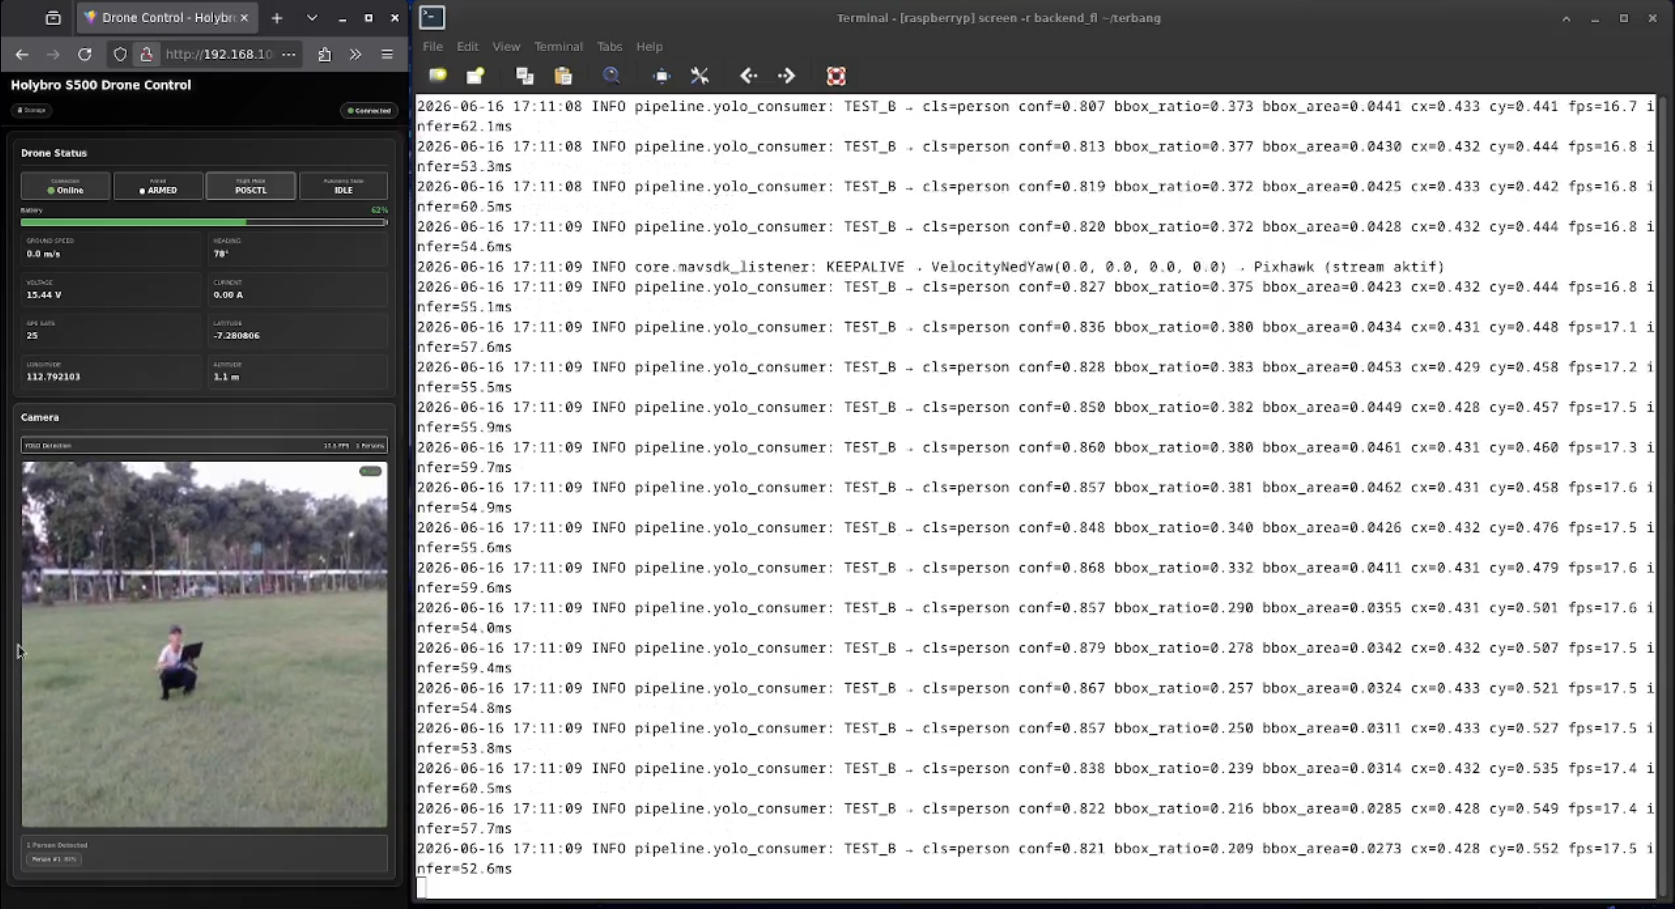
\includegraphics[width=\textwidth]{bab4/fsm_berjalan}
	\caption{Transisi Finite State Machine selama operasi penerbangan}
	\label{fig:fsm_berjalan}
\end{figure}

\subsubsection{Pengujian FSM pada Variasi Posisi Target}

Pengujian validasi FSM sebelumnya dilakukan menggunakan target dengan posisi berdiri. Sebagai pengujian tambahan, pengujian juga dilakukan dengan menggunakan variasi target dalam posisi duduk dan tidur. Pengujian ini bertujuan untuk memvalidasi bahwa transisi \textit{state machine} dari SCAN $\rightarrow$ DETECT $\rightarrow$ APPROACH $\rightarrow$ DOCUMENT $\rightarrow$ DISPLACING $\rightarrow$ RTL tetap berjalan dengan valid tanpa terpengaruh oleh variasi posisi tubuh target. Hasil rekapitulasi pengujian FSM pada variasi posisi target ini disajikan pada Tabel \ref{tab:fsm_variasi_posisi}.

\begin{figure}[H]
	\centering
	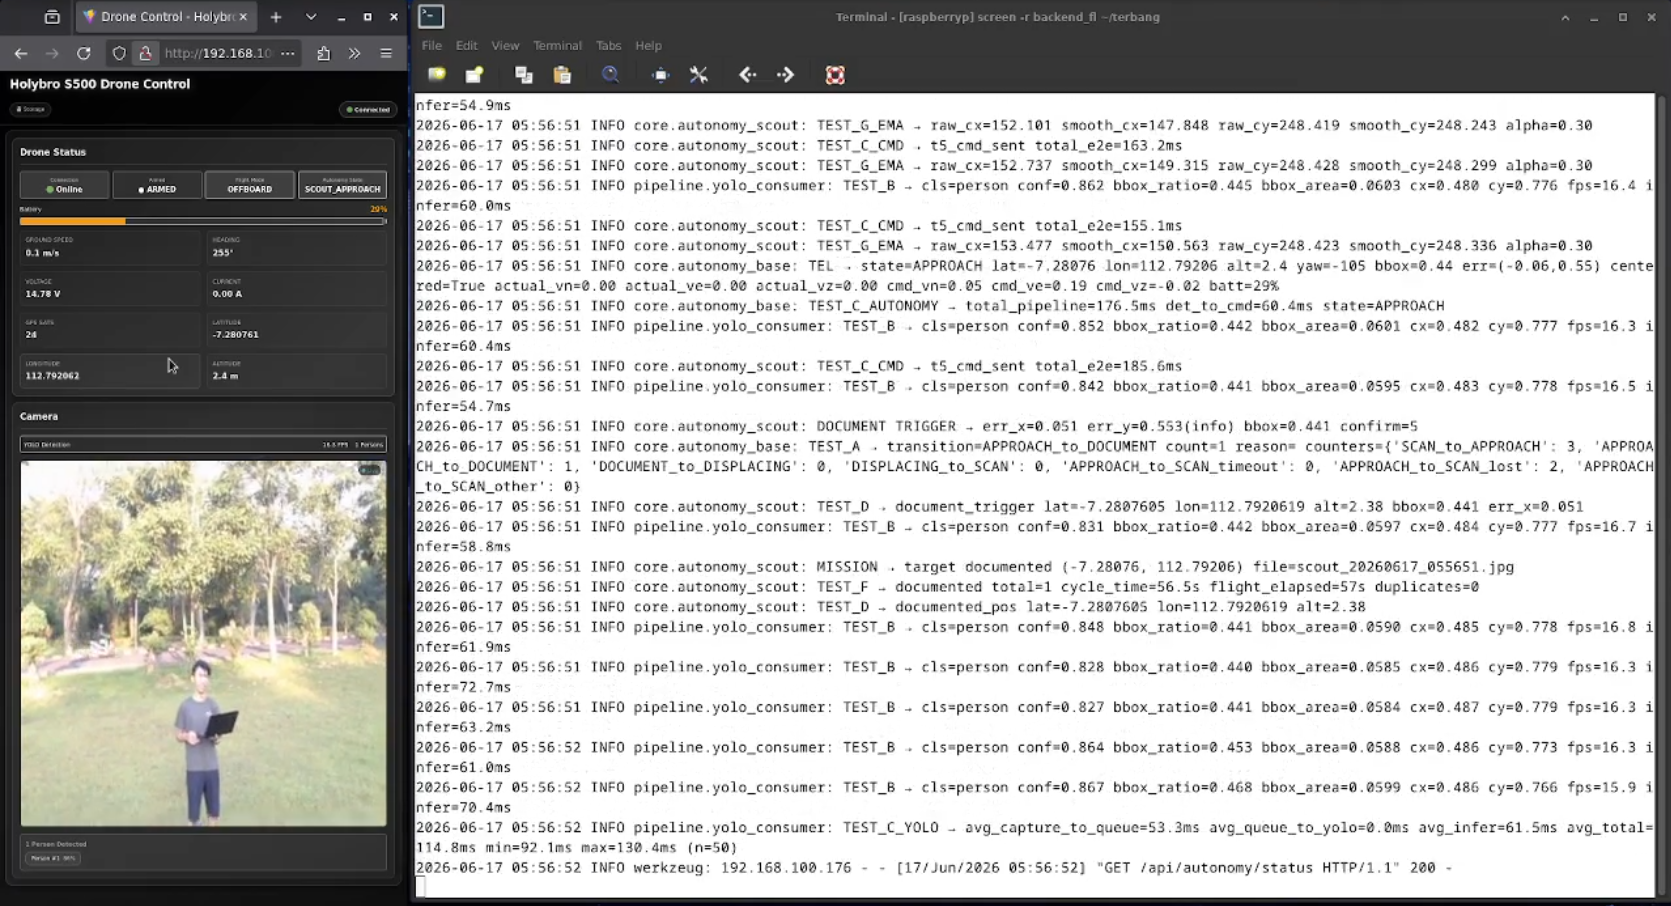
\includegraphics[width=\textwidth]{bab4/fsm_berdiri.png}
	\caption{Hasil pengujian validasi FSM pada posisi target berdiri}
	\label{fig:fsm_berdiri}
\end{figure}

\begin{figure}[H]
	\centering
	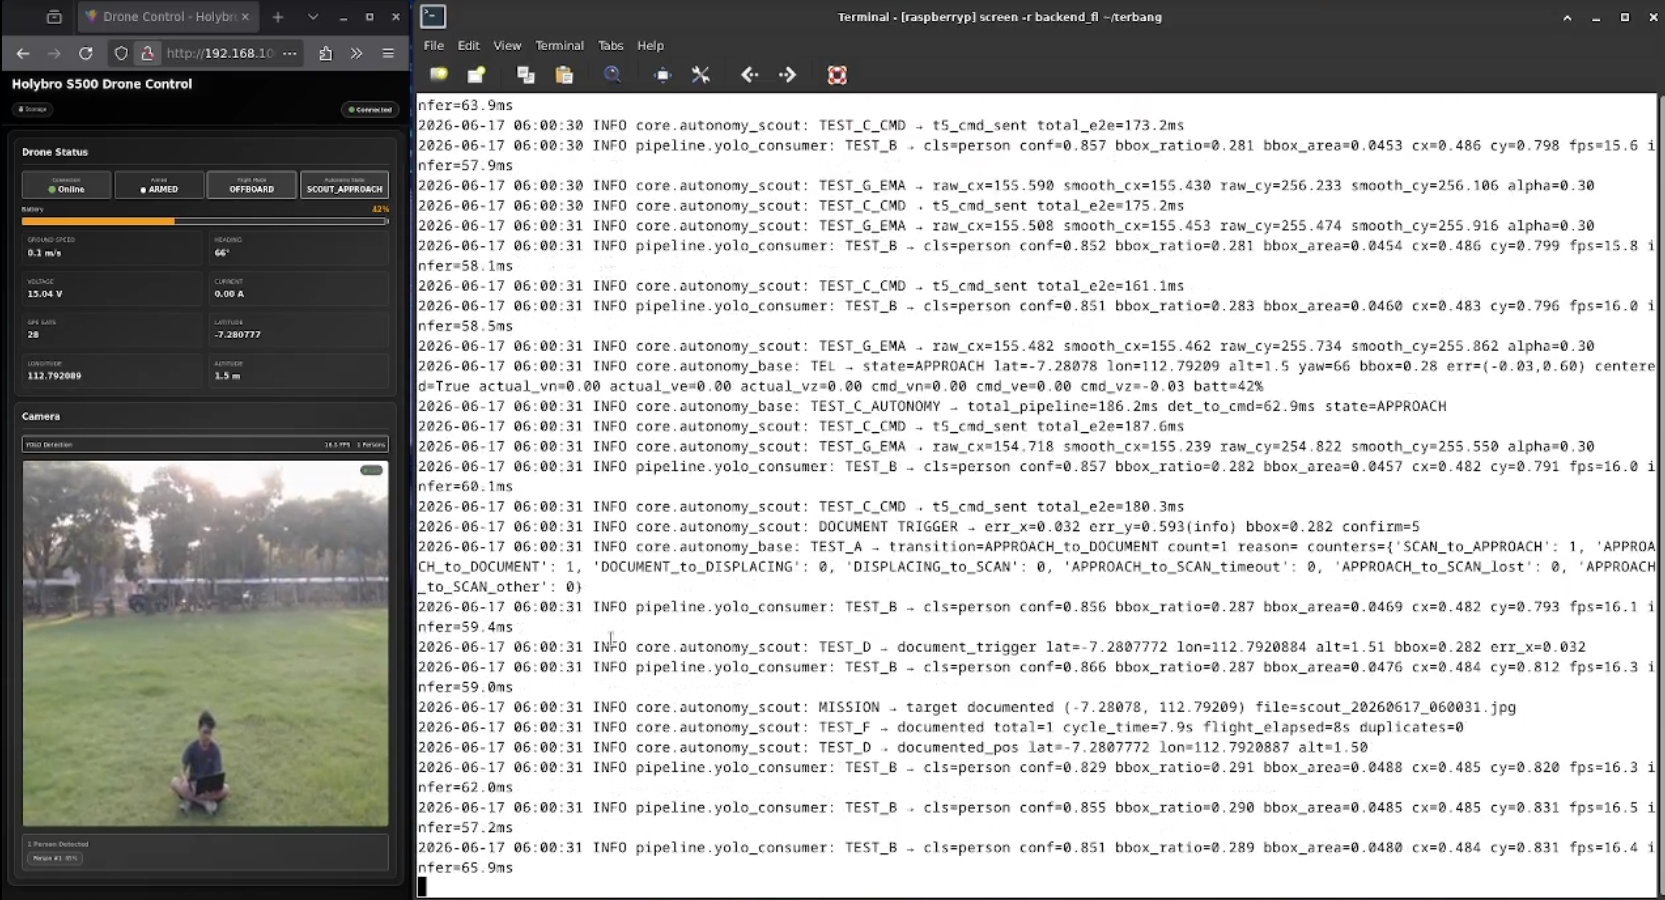
\includegraphics[width=\textwidth]{bab4/fsm_duduk.png}
	\caption{Hasil pengujian validasi FSM pada posisi target duduk}
	\label{fig:fsm_duduk}
\end{figure}

\begin{figure}[H]
	\centering
	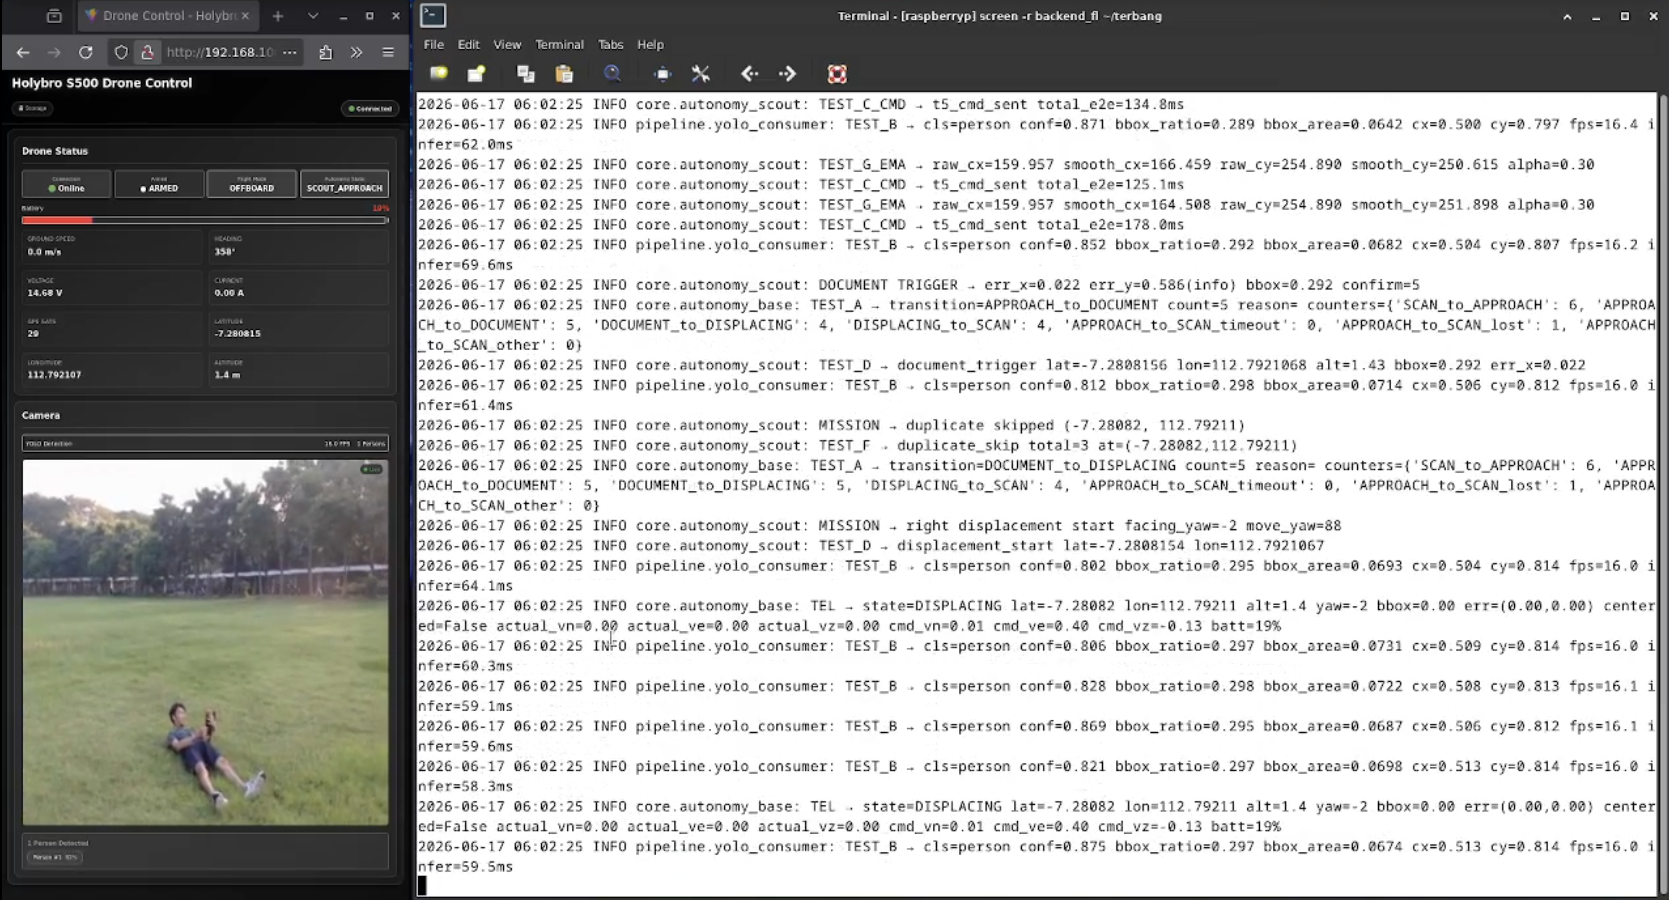
\includegraphics[width=\textwidth]{bab4/fsm_tiduran.png}
	\caption{Hasil pengujian validasi FSM pada posisi target tidur}
	\label{fig:fsm_tidur}
\end{figure}

Visualisasi pada Gambar \ref{fig:fsm_berdiri}, Gambar \ref{fig:fsm_duduk}, dan Gambar \ref{fig:fsm_tidur} mendemonstrasikan stabilitas deteksi YOLOv8n hasil \textit{fine-tuning} terhadap orientasi target manusia (berdiri, duduk, berjalan, dan tidur). Kestabilan kotak pembatas (\textit{bounding box}) sangat bergantung pada kelengkapan fitur visual tubuh korban yang tertangkap oleh sensor kamera. Pada posisi tegak seperti berdiri dan berjalan, deteksi menunjukkan konsistensi tinggi karena pola geometris tubuh selaras dengan dataset latih. Sebaliknya, pada posisi duduk atau tidur, deteksi dipengaruhi oleh sudut datang (\textit{angle of attack}) kamera drone yang berpotensi menimbulkan oklusi parsial pada ekstremitas tubuh. Meski demikian, model optimasi ini tetap mempertahankan kestabilan deteksi yang memadai untuk transisi keadaan otonom secara tepat.

\begin{table}[H]
	\centering
	\caption{Hasil Pengujian Validasi State Machine pada Variasi Posisi Target}
	\label{tab:fsm_variasi_posisi}
	\renewcommand{\arraystretch}{1.0}
	\resizebox{\textwidth}{!}{
	\begin{tabular}{|l|c|c|c|c|c|p{3.5cm}|}
		\hline
		\textbf{Posisi Target} & \textbf{Scan} & \textbf{Approach} & \textbf{Document} & \textbf{Displacing} & \textbf{RTL} & \textbf{Keterangan} \\ \hline
		Berdiri & Ya & Ya & Ya & Ya & Ya & Seluruh tahapan FSM berhasil dijalankan tanpa kendala. \\ \hline
		Duduk & Ya & Ya & Ya & Ya & Ya & Seluruh tahapan FSM berhasil dijalankan tanpa kendala. \\ \hline
		Tidur & Ya & Ya & Ya & Ya & Ya & Deteksi berhasil ketika tubuh terlihat dari sisi kanan atau kiri sehingga kepala, badan, dan kaki dapat diamati secara bersamaan. \\ \hline
	\end{tabular}
	}
\end{table}

Pengujian menunjukkan bahwa sistem mampu menyelesaikan seluruh rangkaian \textit{state} misi pada target dengan posisi berdiri maupun duduk. Pada kedua kondisi tersebut, tubuh manusia masih terlihat dengan proporsi yang cukup lengkap dari sudut pandang kamera sehingga objek dapat dideteksi secara konsisten oleh model. Setelah target terdeteksi, FSM berhasil melakukan transisi dari \texttt{SCAN} menuju \texttt{APPROACH}, \texttt{DOCUMENT}, \texttt{DISPLACING}, hingga \texttt{RTL} tanpa kendala yang berarti.

Pada posisi tidur, karakteristik deteksi menunjukkan perbedaan. Deteksi manusia cenderung berhasil ketika kamera menangkap sebagian besar bentuk tubuh dari kepala hingga kaki, khususnya dari sisi lateral target. Sebaliknya, saat drone sejajar dengan sumbu longitudinal target (misalnya tepat di belakang kepala atau di depan kaki), objek manusia sering tidak terdeteksi karena fitur visual pada citra sangat terbatas dan tidak menyerupai representasi tubuh manusia pada umumnya.

Seiring pergerakan drone selama proses pencarian, sudut pandang kamera berubah sehingga bagian kepala, badan, dan kaki mulai terlihat secara bersamaan dari sisi tubuh target. Pada kondisi tersebut deteksi kembali berhasil dilakukan dan FSM dapat melanjutkan transisi ke tahapan misi berikutnya. Hasil ini menunjukkan bahwa keberhasilan sistem tidak hanya dipengaruhi oleh posisi tubuh target, tetapi juga oleh sudut pengamatan kamera terhadap target selama proses pencarian berlangsung.


\subsection{Skenario B: Pengujian Akurasi Deteksi In-Flight (Airborne Detection Performance)}

Pengujian performa deteksi saat penerbangan sesungguhnya (\textit{in-flight}) dilakukan untuk mengevaluasi kemampuan model YOLOv8n dalam mendeteksi manusia ketika drone berada pada kondisi operasi nyata. Pengujian dilaksanakan dengan drone melayang (\textit{hover}) pada ketinggian sekitar 1--2 meter di atas permukaan tanah (AGL), sedangkan target manusia bergerak menjauh secara bertahap hingga mencapai jarak sekitar 20 meter dari posisi drone.

Penentuan jarak target dilakukan melalui sinkronisasi video streaming hasil penerbangan dengan pengamatan visual serta pengukuran lapangan menggunakan Google Maps. Data log deteksi kemudian diekstraksi berdasarkan rentang waktu saat target berada pada jarak tertentu dari UAV. Metrik yang dianalisis meliputi \textit{Detection Rate}, rata-rata nilai \textit{confidence}, rata-rata ukuran \textit{bounding box}, serta performa FPS selama inferensi berlangsung.

Hasil pengujian membuktikan tingkat deteksi 100\% dapat dipertahankan hingga jarak 15 meter karena ukuran target pada citra masih cukup besar. Pada jarak 20 meter, penyusutan dimensi visual target menurunkan tingkat deteksi menjadi 45,5\%. Penurunan ini terkonfirmasi dari menyusutnya rata-rata luas kotak pembatas (\textit{bounding box area}) dari 0,0479 (jarak 5 meter) menjadi hanya 0,0067 (jarak 20 meter), seperti diperbandingkan secara visual pada Gambar \ref{fig:deteksi_in_flight}.

Meskipun nilai \textit{confidence} deteksi tetap berada pada kisaran 0,74--0,82, frekuensi kemunculan deteksi menjadi semakin jarang pada jarak yang lebih jauh. Berdasarkan hasil tersebut, jarak operasional yang paling optimal untuk memulai manuver \textit{APPROACH} berada pada rentang hingga 15 meter dari target. Rekapitulasi metrik deteksi manusia saat penerbangan pada berbagai jarak disajikan secara kuantitatif pada Tabel \ref{tab:inflight_detection}.

\begin{figure}[H]
	\centering
	\begin{subfigure}{\textwidth}
		\centering
		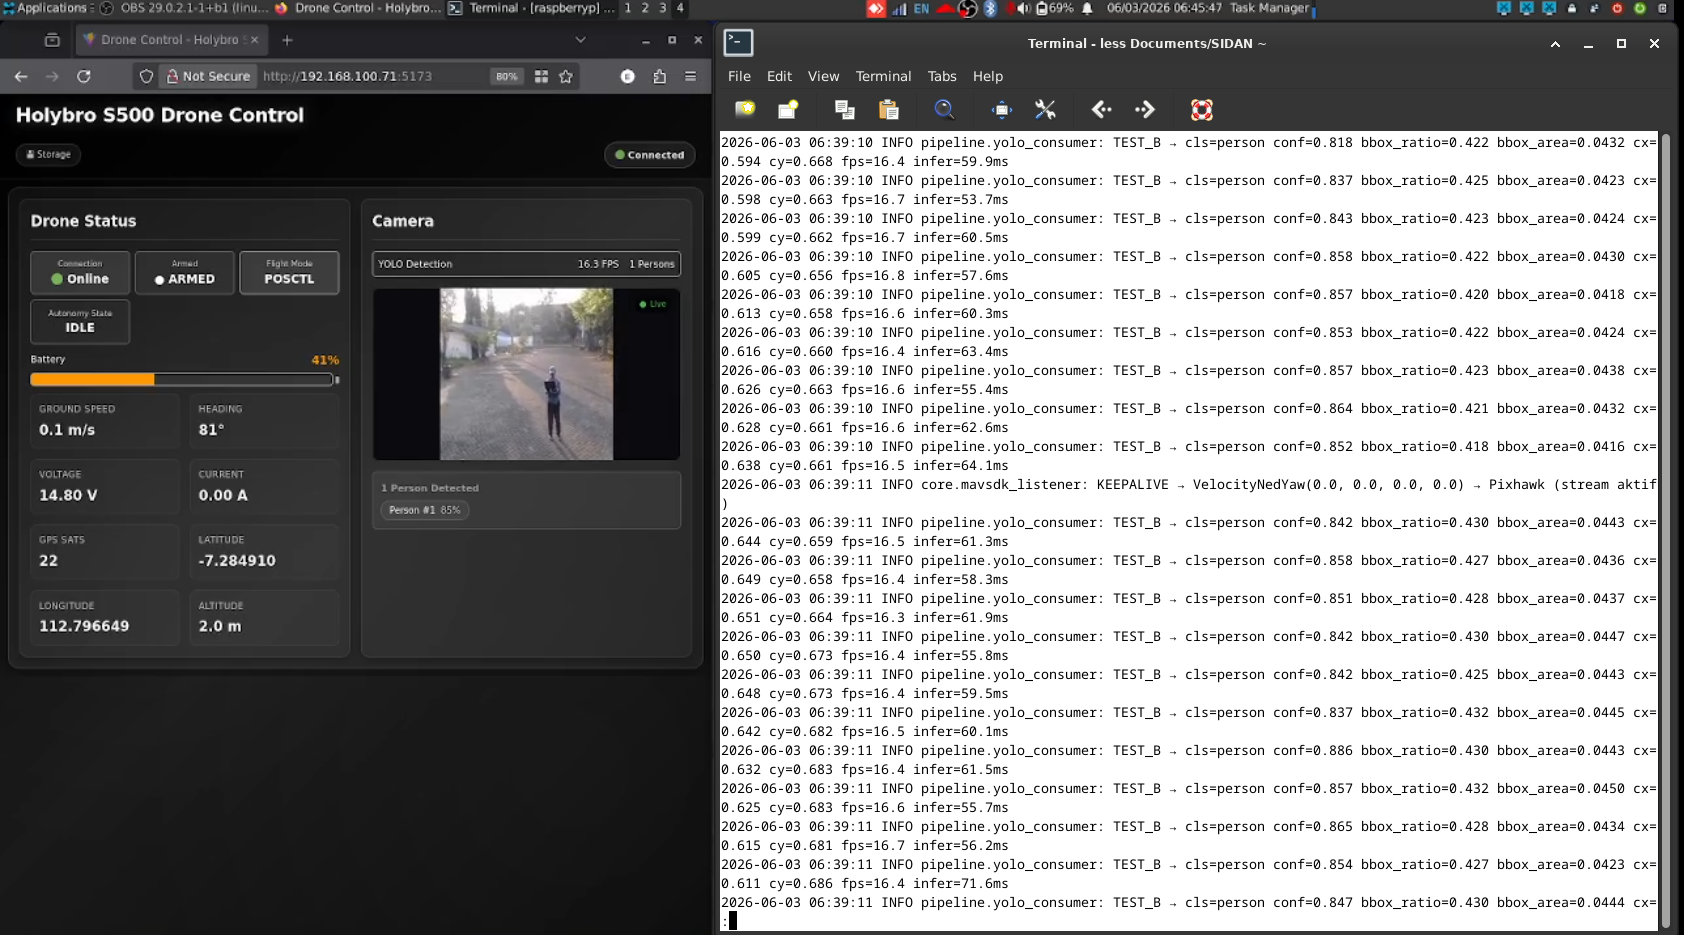
\includegraphics[width=\textwidth]{bab4/deteksi5m}
		\caption{Deteksi pada jarak 5 meter}
	\end{subfigure}
	\hfill
	\begin{subfigure}{\textwidth}
		\centering
		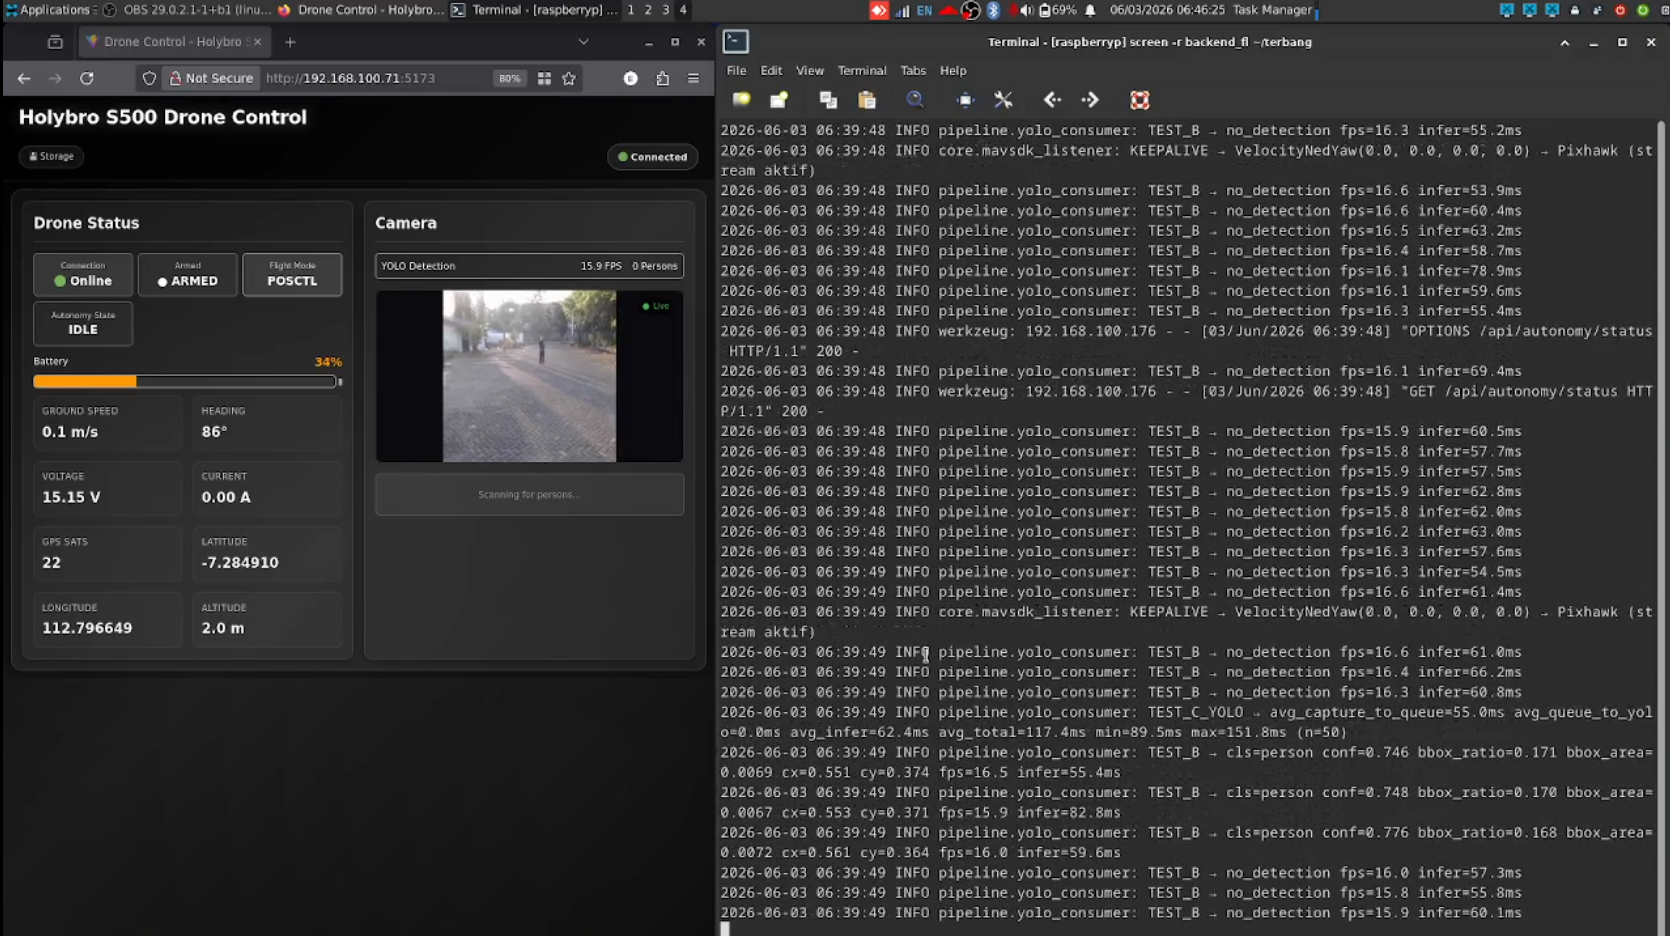
\includegraphics[width=\textwidth]{bab4/deteksi20m}
		\caption{Deteksi pada jarak 20 meter}
	\end{subfigure}
	\caption{Perbandingan deteksi target pada jarak 5 meter dan 20 meter}
	\label{fig:deteksi_in_flight}
\end{figure}

\begin{table}[H]
	\centering
	\caption{Hasil Pengujian Akurasi Deteksi In-Flight}
	\label{tab:inflight_detection}
	\renewcommand{\arraystretch}{1.2}
	\small
	\begin{tabular}{|c|c|c|c|c|}
		\hline
		\textbf{Jarak Target (m)} &
		\textbf{Detection Rate (\%)} &
		\textbf{Avg Confidence} &
		\textbf{Avg BBox Area} &
		\textbf{Avg FPS}
		\\ \hline
		
		5 &
		100.0 &
		0.821 &
		0.0479 &
		16.51
		\\ \hline
		
		10 &
		100.0 &
		0.766 &
		0.0169 &
		16.46
		\\ \hline
		
		15 &
		100.0 &
		0.747 &
		0.0100 &
		16.51
		\\ \hline
		
		20 &
		45.5 &
		0.749 &
		0.0067 &
		16.46
		\\ \hline
		
	\end{tabular}
\end{table}

Berdasarkan hasil pengujian, ukuran target pada citra memiliki pengaruh yang lebih besar terhadap keberhasilan deteksi dibandingkan nilai \textit{confidence} model. Ketika target semakin jauh, ukuran \textit{bounding box} terus mengecil sehingga frekuensi deteksi menurun walaupun model masih memberikan nilai \textit{confidence} yang relatif tinggi. Oleh karena itu, jarak efektif deteksi manusia pada konfigurasi sistem yang digunakan dalam penelitian ini berada pada kisaran hingga 15 meter dengan tingkat keberhasilan deteksi yang konsisten, sedangkan pada jarak sekitar 20 meter deteksi mulai mengalami penurunan yang signifikan.

\subsection{Skenario C: Pengujian Latensi Pipeline End-to-End}

Pengujian ini mengukur latensi dari akuisisi citra hingga pengiriman perintah Pixhawk menggunakan penanda \texttt{TEST\_C\_YOLO}, \texttt{TEST\_C\_AUTONOMY}, dan \texttt{TEST\_C\_CMD} pada lima penerbangan (2096 sampel).

Hasil pengujian menunjukkan bahwa rata-rata waktu akuisisi frame dari kamera hingga masuk ke antrean pemrosesan sebesar 41,87 ms. Proses inferensi YOLOv8n320 ONNX memiliki rata-rata latensi 59,08 ms dengan deviasi standar 4,42 ms, menunjukkan performa inferensi yang relatif stabil selama penerbangan. Selain itu, latensi antrean menuju proses inferensi tercatat mendekati nol karena frame yang masuk ke queue langsung dikonsumsi oleh \textit{thread} inferensi sehingga tidak terjadi backlog yang signifikan.

Tahap dengan variasi latensi terbesar terjadi pada proses pengolahan deteksi hingga pembangkitan perintah navigasi (\textit{Detection to Command Generation}) dengan rata-rata 73,34 ms dan nilai maksimum mencapai 1380,1 ms. Variasi tersebut menunjukkan adanya beberapa kejadian \textit{outlier} yang kemungkinan dipengaruhi oleh penjadwalan \textit{thread} sistem operasi, kondisi beban komputasi, atau penumpukan proses pada siklus tertentu.

Secara keseluruhan, rata-rata latensi \textit{end-to-end} dari penangkapan frame hingga pengiriman perintah \textit{VelocityNedYaw} ke Pixhawk adalah 188,04 ms. Analisis distribusi latensi menunjukkan bahwa median (P50) latensi berada pada 164,65 ms, sedangkan 95\% sampel berada di bawah 208,27 ms. Meskipun ditemukan beberapa \textit{outlier} dengan latensi maksimum sebesar 1602,2 ms, mayoritas siklus pemrosesan sistem tetap berada pada rentang 160--210 ms sehingga masih memenuhi kebutuhan kendali drone pada kecepatan rendah hingga menengah.

\begin{table}[H]
	\centering
	\caption{Hasil Pengujian Latensi Pipeline End-to-End}
	\label{tab:pipeline_latency}
	\renewcommand{\arraystretch}{1.2}
	\small
	\resizebox{\textwidth}{!}{
	\begin{tabular}{|l|c|c|c|c|}
		\hline
		\textbf{Stage Pipeline} & \textbf{Rata-rata Latensi (ms)} & \textbf{Min (ms)} & \textbf{Max (ms)} & \textbf{Std Dev (ms)} \\ \hline
		Capture $\rightarrow$ Frame Queue & 41,87 & 0,5 & 57,4 & 21,45 \\ \hline
		Frame Queue $\rightarrow$ YOLO Start & 0,00 & 0,0 & 0,0 & 0,00 \\ \hline
		YOLO Inferensi & 59,08 & 49,9 & 76,8 & 4,42 \\ \hline
		Detection $\rightarrow$ Command Generation & 73,34 & 1,2 & 1380,1 & 164,71 \\ \hline
		\textbf{Total End-to-End} & \textbf{188,04} & \textbf{53,0} & \textbf{1602,2} & \textbf{185,10} \\ \hline
	\end{tabular}
	}
\end{table}

Dari Tabel \ref{tab:pipeline_latency}, meskipun rata-rata latensi total (\textit{End-to-End}) adalah 188,04 ms, tahap pemrosesan inferensi YOLOv8n dan pengiriman perintah navigasi mendominasi sekitar 70\% dari total waktu tunda tersebut. Karakteristik ini diduga dipengaruhi oleh keterbatasan akselerasi perangkat keras (\textit{hardware acceleration}) pada CPU Raspberry Pi 5 saat melakukan inferensi model visi komputer secara terus-menerus.

Untuk memberikan gambaran distribusi latensi yang lebih representatif, dilakukan pula analisis persentil terhadap latensi \textit{end-to-end} sebagaimana ditunjukkan pada Tabel \ref{tab:e2e_percentile}. Pembagian persentil ini membantu memetakan batas atas waktu tunggu (latensi) pada sebagian besar sampel data pengujian. Melalui analisis statistik sebaran data ini, stabilitas pemrosesan asinkron drone otonom dapat dibuktikan secara lebih valid.

\begin{table}[H]
	\centering
	\caption{Distribusi Persentil Latensi End-to-End}
	\label{tab:e2e_percentile}
	\renewcommand{\arraystretch}{1.2}
	\begin{tabular}{|c|c|}
		\hline
		\textbf{Persentil} & \textbf{Latensi (ms)} \\ \hline
		P50 (Median) & 164,65 \\ \hline
		P90 & 192,30 \\ \hline
		P95 & 208,27 \\ \hline
		P99 & 1293,13 \\ \hline
	\end{tabular}
\end{table}

Distribusi data persentil pada Tabel \ref{tab:e2e_percentile} mengonfirmasi bahwa mayoritas siklus pemrosesan terkonsentrasi di bawah batas kritis 200 ms. Nilai pencilan ekstrem hanya terjadi pada persentil tertinggi (P99) akibat interupsi komputasi transien dari kernel sistem operasi. Karakteristik latensi yang stabil ini mendukung responsivitas kendali navigasi otonom agar tetap presisi selama manuver drone berlangsung. Selanjutnya, stabilitas respons navigasi dievaluasi secara geometris melalui akurasi pendekatan dan perpindahan spasial drone.

\subsection{Skenario D: Pengujian Akurasi Navigasi Otonom (Approach \& Displacement Accuracy)}

Pengujian ini bertujuan untuk mengevaluasi kualitas pendekatan (\textit{approach}) terhadap target manusia serta akurasi manuver perpindahan lateral (\textit{displacement}) yang dilakukan setelah proses dokumentasi selesai. Karena target manusia bergerak selama pengujian, akurasi pendekatan tidak dievaluasi menggunakan deviasi GPS terhadap posisi target. Sebagai gantinya, kualitas pendekatan dinilai berdasarkan kondisi target pada saat \textit{document trigger} dieksekusi, yaitu menggunakan nilai \textit{bounding box ratio} dan kesalahan horizontal target terhadap pusat citra (\textit{horizontal alignment error}, \texttt{err\_x}).

Nilai \textit{bounding box ratio} menunjukkan proporsi ukuran target terhadap bidang pandang kamera, sedangkan \texttt{err\_x} menunjukkan seberapa dekat posisi target terhadap pusat frame pada saat dokumentasi dilakukan. Semakin besar nilai \textit{bounding box ratio} dan semakin kecil nilai \texttt{err\_x}, maka semakin baik kualitas pendekatan yang dicapai oleh sistem.

\begin{table}[H]
	\centering
	\caption{Hasil Pengujian Kualitas Pendekatan (\textit{Approach Trigger Quality})}
	\label{tab:approach_accuracy}
	\renewcommand{\arraystretch}{1.2}
	\begin{tabular}{|l|c|}
		\hline
		\textbf{Parameter} & \textbf{Nilai} \\ \hline
		Jumlah Trigger Dokumentasi & 30 \\ \hline
		Rata-rata BBox Ratio & 0.389 \\ \hline
		Rata-rata Horizontal Error (\texttt{err\_x}) & 0.049 \\ \hline
	\end{tabular}
\end{table}

Hasil pengujian menunjukkan bahwa sistem mampu membawa target ke area terpusat pada citra dengan proporsi ukuran yang ideal sebelum \textit{document trigger} dieksekusi (visualisasi tangkapan layar saat modul navigasi menyejajarkan posisi dengan target ditunjukkan pada Gambar \ref{fig:document_triggered}). Detail metrik pengujian pendekatan target dapat dilihat secara utuh pada Tabel \ref{tab:approach_accuracy}.

\begin{figure}[H]
	\centering
	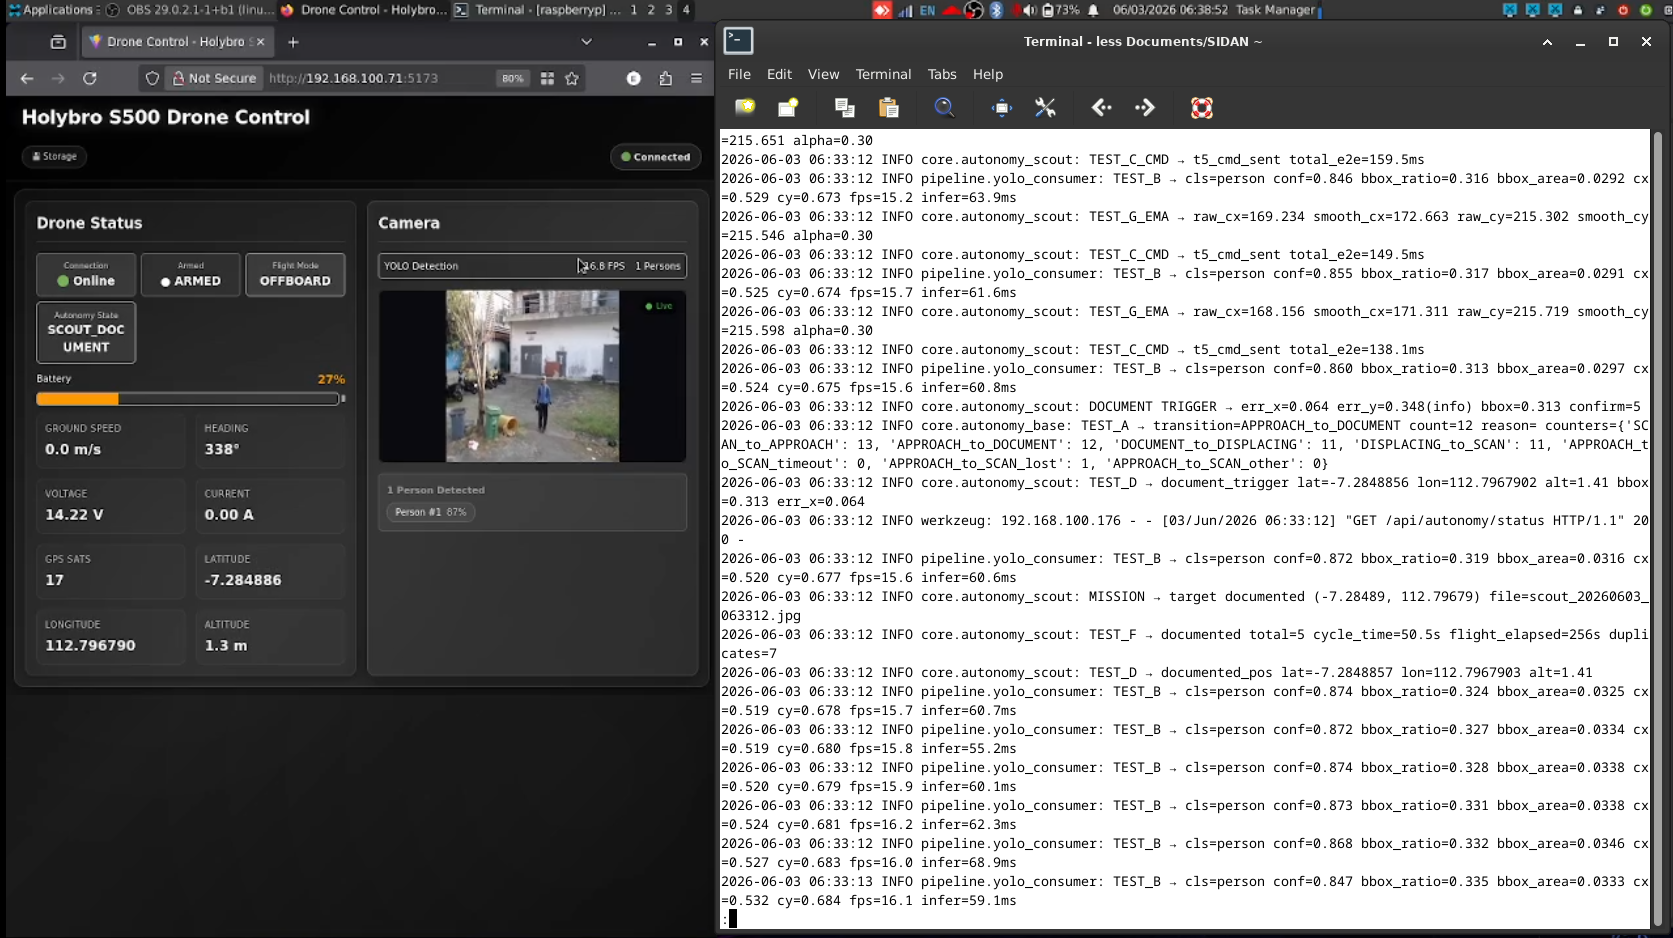
\includegraphics[width=\textwidth]{bab4/document_triggered}
	\caption{Tangkapan layar saat \textit{document trigger} dieksekusi}
	\label{fig:document_triggered}
\end{figure}

Selain kualitas pendekatan, akurasi manuver perpindahan lateral dievaluasi menggunakan data GPS yang direkam pada event \texttt{displacement\_start} dan \texttt{displacement\_end}. Sistem dirancang untuk melakukan perpindahan sejauh 2 meter setelah proses dokumentasi selesai. Jarak aktual perpindahan dihitung secara otomatis oleh sistem dan dibandingkan terhadap jarak target untuk memperoleh nilai error.

\begin{table}[H]
	\centering
	\caption{Hasil Pengujian Akurasi Displacement}
	\label{tab:displacement_accuracy}
	\renewcommand{\arraystretch}{1.2}
	\begin{tabular}{|l|c|}
		\hline
		\textbf{Parameter} & \textbf{Nilai} \\ \hline
		Jumlah Percobaan & 29 \\ \hline
		Jarak Target (m) & 2.0 \\ \hline
		Rata-rata Jarak Aktual (m) & 1.99 \\ \hline
		Rata-rata Error (m) & 0.09 \\ \hline
		Rata-rata Error (\%) & 4.52 \\ \hline
	\end{tabular}
\end{table}

Sistem terbukti mampu melakukan manuver perpindahan lateral dengan tingkat akurasi yang tinggi dan konsisten, menghasilkan deviasi marjinal di bawah 5\% sebagaimana ditunjukkan pada Tabel \ref{tab:displacement_accuracy}. Presisi ini sangat krusial untuk mendukung proses pencarian target berikutnya tanpa mengakumulasi simpangan posisi spasial.

Tingkat keberhasilan relokasi (\textit{displacement accuracy}) otonom yang tinggi ini secara langsung berdampak positif pada efisiensi perluasan area pencarian korban. Dengan simpangan lateral yang sangat minim, drone dapat menyapu area bencana secara sistematis tanpa mengalami penumpukan area observasi yang redundan. Efektivitas pencarian taktis ini memastikan bahwa sumber daya energi baterai dapat dialokasikan secara optimal untuk menjangkau radius pencarian yang lebih luas. Oleh karena itu, presisi navigasi otonom pada fase \textit{displacement} ini terbukti menjadi kunci utama dalam mempercepat penemuan korban SAR. Untuk mengimbangi agresivitas manuver otonom tersebut, jaminan keselamatan penerbangan menjadi prioritas mutlak. Skenario berikutnya membahas keandalan mekanisme perlindungan drone dalam menghadapi berbagai kondisi anomali operasional.

\subsection{Skenario E: Pengujian Respons Safety Override dan Safety System}

Pengujian ini bertujuan untuk memvalidasi efektivitas mekanisme keselamatan dan prosedur respons darurat (\textit{emergency response procedure}) yang diimplementasikan pada platform otonom. Validasi dilakukan menggunakan data log penerbangan aktual yang mencakup aktivasi \textit{Battery RTL}, \textit{Pre-RTL Safety Climb}, \textit{RC Override}, dan \textit{OFFBOARD Exit Handling}. Hasil pengujian menunjukkan bahwa seluruh mekanisme keselamatan berhasil terpicu sesuai kondisi yang dirancang dan mampu mencegah kondisi operasi yang berpotensi membahayakan drone.

\begin{enumerate}
	\item \textit{Battery RTL}: Sistem secara otomatis mengaktifkan prosedur pemulangan ketika kapasitas baterai mencapai ambang kritis. Mekanisme ini berhasil terpicu pada Flight~1, Flight~2, dan Flight~3.
	
	\item \textit{Pre-RTL Safety Climb}: Setelah \textit{Battery RTL} terdeteksi, sistem menghentikan pergerakan horizontal dan melakukan pendakian vertikal sebelum mengirim perintah RTL ke PX4. Pengujian dilakukan dengan mengukur durasi manuver pendakian dan ketinggian tambahan yang dicapai selama proses pendakian pengamanan.
	
	\item \textit{RC Override}: Intervensi operator dengan beralih ke mode \texttt{POSCTL} berhasil membatalkan sistem otonom secara paksa dan mengembalikan kontrol penuh.
	
	\item \textit{OFFBOARD Exit Handling}: Saat sistem keluar dari mode OFFBOARD, proses otonom langsung dihentikan sehingga tidak ada perintah navigasi yang tetap berjalan tanpa pengawasan operator.
\end{enumerate}

Sebelum memaparkan hasil pengujian pada Tabel~\ref{tab:safety_pre_rtl}, perlu ditegaskan bahwa pengujian fitur \textit{Battery RTL} ini sama sekali tidak bertujuan untuk mengevaluasi kinerja algoritma estimasi energi UAV yang adaptif. Pengembangan ini murni menggunakan nilai batas tetap (\textit{fixed threshold}) yang ditetapkan secara konstan sebesar 15\% baterai. Oleh karena itu, pengujian yang dilakukan difokuskan untuk memvalidasi keberhasilan aktivasi mekanisme pemulangan otomatis (\textit{Battery RTL Mechanism}) baterai kritis, yang meliputi keberhasilan penghentian misi aktif (\textit{mission abortion}), eksekusi manuver \textit{Pre-RTL Safety Climb}, transisi menuju mode penerbangan RTL bawaan PX4, serta jaminan keamanan operasional drone secara keseluruhan selama proses penyelamatan darurat berlangsung.

\begin{table}[H]
	\centering
	\caption{Hasil Pengujian Battery RTL dan Pre-RTL Safety Climb}
	\label{tab:safety_pre_rtl}
	\renewcommand{\arraystretch}{1.2}
	\small
	\begin{tabular}{|c|c|c|c|c|}
		\hline
		\textbf{Flight} &
		\textbf{Durasi Manuver (ms)} &
		\textbf{Expected Gain (m)} &
		\textbf{Actual Gain (m)} &
		\textbf{Outcome}
		\\ \hline
		
		1 & 3017 & 2.40 & 2.27 & PASS \\ \hline
		2 & 2006 & 1.60 & 0.46 & PASS \\ \hline
		3 & 2029 & 1.60 & 1.34 & PASS \\ \hline
		
	\end{tabular}
\end{table}

Berdasarkan hasil observasi, deviasi pemicuan \textit{Battery RTL} aktif pada kisaran 13\%--14\% meskipun threshold dikonfigurasi 15\% diduga dipengaruhi oleh interval pembaruan telemetri asinkron MAVSDK Listener, frekuensi loop autonomi 20 Hz, latensi transmisi MAVLink, serta fenomena \textit{voltage sag} (penurunan tegangan sementara) akibat lonjakan beban dinamis motor drone saat manuver terbang. 

Selain itu, durasi manuver pendakian pada Flight~2 (2006 ms) dan Flight~3 (2029 ms) terindikasi mengalami terminasi lebih awal dibandingkan target konfigurasi statis \texttt{SCOUT\_PRE\_RTL\_CLIMB\_S} = 3,0 detik (seperti pada Flight~1). Salah satu faktor yang dapat memengaruhi kondisi ini adalah aktifnya proteksi baterai kritis internal PX4 secara mandiri pada level 13\%--14\%, yang kemungkinan menyebabkan penolakan perintah setpoint OFFBOARD vertikal dari Raspberry Pi 5. Akibatnya, fungsi \texttt{set\_velocity\_ned} mendeteksi kegagalan komunikasi kontrol (\textit{offboard exception}) dan melakukan keluar awal (\textit{break}) dari loop pendakian. Deviasi pendakian aktual pada Flight~2 yang hanya mencapai 0,46 meter diduga dipicu oleh penurunan daya dorong instan baterai di bawah beban dinamis tinggi, namun integrasi sistem tetap dinilai aman (\textit{PASS}) karena kendali penerbangan berhasil dialihkan sepenuhnya ke mode PX4 RTL. Sementara itu, rekapitulasi keberhasilan pengujian mekanisme intervensi manual (RC Override) dan pemutusan kendali otonom (OFFBOARD Exit) disajikan pada Tabel \ref{tab:safety_override}.

\begin{table}[H]
	\centering
	\caption{Hasil Pengujian RC Override dan OFFBOARD Exit Handling}
	\label{tab:safety_override}
	\renewcommand{\arraystretch}{1.2}
	\small
	\begin{tabular}{|c|c|c|}
		\hline
		\textbf{Mechanism} &
		\textbf{Flight} &
		\textbf{Outcome}
		\\ \hline
		
		RC Override & 2 & PASS \\ \hline
		RC Override & 4 & PASS \\ \hline
		RC Override & 5 & PASS \\ \hline
		
		OFFBOARD Exit & 2 & PASS \\ \hline
		OFFBOARD Exit & 4 & PASS \\ \hline
		OFFBOARD Exit & 5 & PASS \\ \hline
		
	\end{tabular}
\end{table}

Selain evaluasi kuantitatif, keandalan sistem keselamatan divalidasi secara kualitatif lewat rekaman log penerbangan. Aktivasi \textit{Battery RTL} ditandai oleh log berikut:

\begin{quote}
	\texttt{TEST\_E -> battery\_rtl\_trigger batt=14.0\%}
\end{quote}

Setelah kondisi tersebut terdeteksi, sistem menjalankan prosedur pendakian pengamanan yang ditandai dengan log:

\begin{quote}
	\texttt{TEST\_E -> pre\_rtl\_complete response\_time=2006ms}
\end{quote}

Intervensi operator tervalidasi melalui log:

\begin{quote}
	\texttt{Flight mode -> POSCTL: stopping autonomy}
\end{quote}

Sedangkan penanganan keluarnya mode OFFBOARD dibuktikan oleh log:

\begin{quote}
	\texttt{OFFBOARD EXITED -> Autonomy Stopped}
\end{quote}

Berdasarkan hasil pengujian kuantitatif dan bukti kualitatif yang diperoleh dari log penerbangan, seluruh mekanisme keselamatan berhasil beroperasi sesuai tujuan perancangannya. Sistem mampu mendeteksi kondisi baterai kritis, menjalankan prosedur pendakian pengamanan sebelum RTL, menghentikan operasi otonom saat terjadi intervensi operator, serta menangani keluarnya mode OFFBOARD tanpa menimbulkan kondisi yang berpotensi membahayakan drone.

\begin{figure}[H]
	\centering
	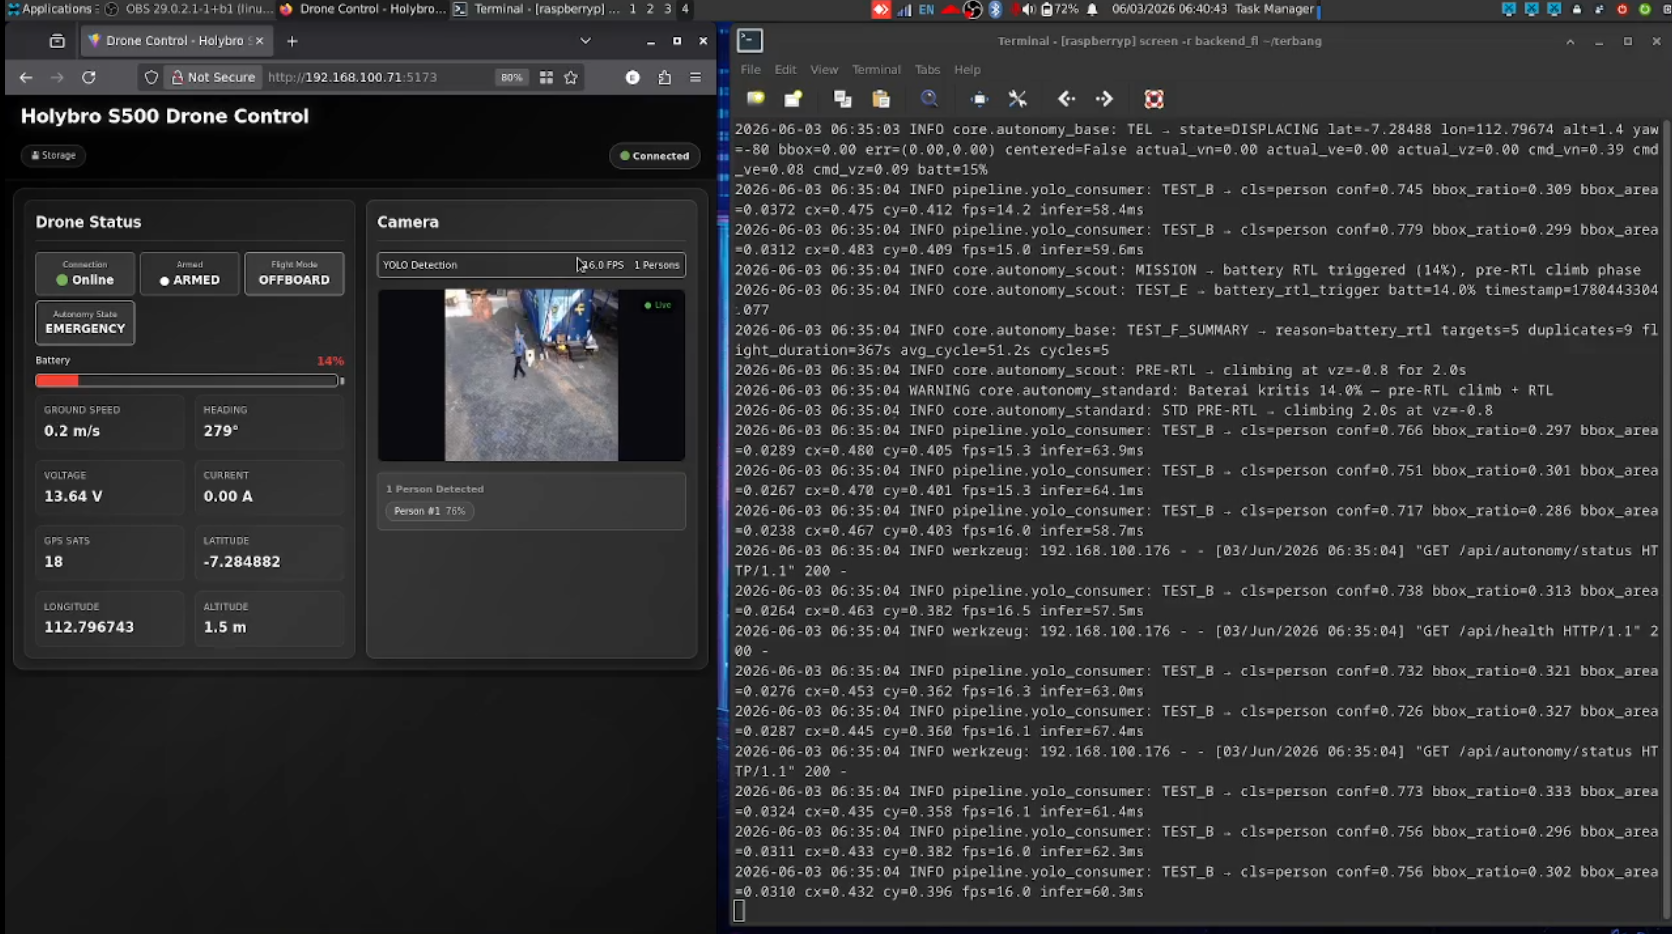
\includegraphics[width=\textwidth]{bab4/battery_rtl_trigggered}
	\caption{Pemicu Battery RTL}
	\label{fig:battery_rtl}
	
	\vspace{0.5cm}
	
	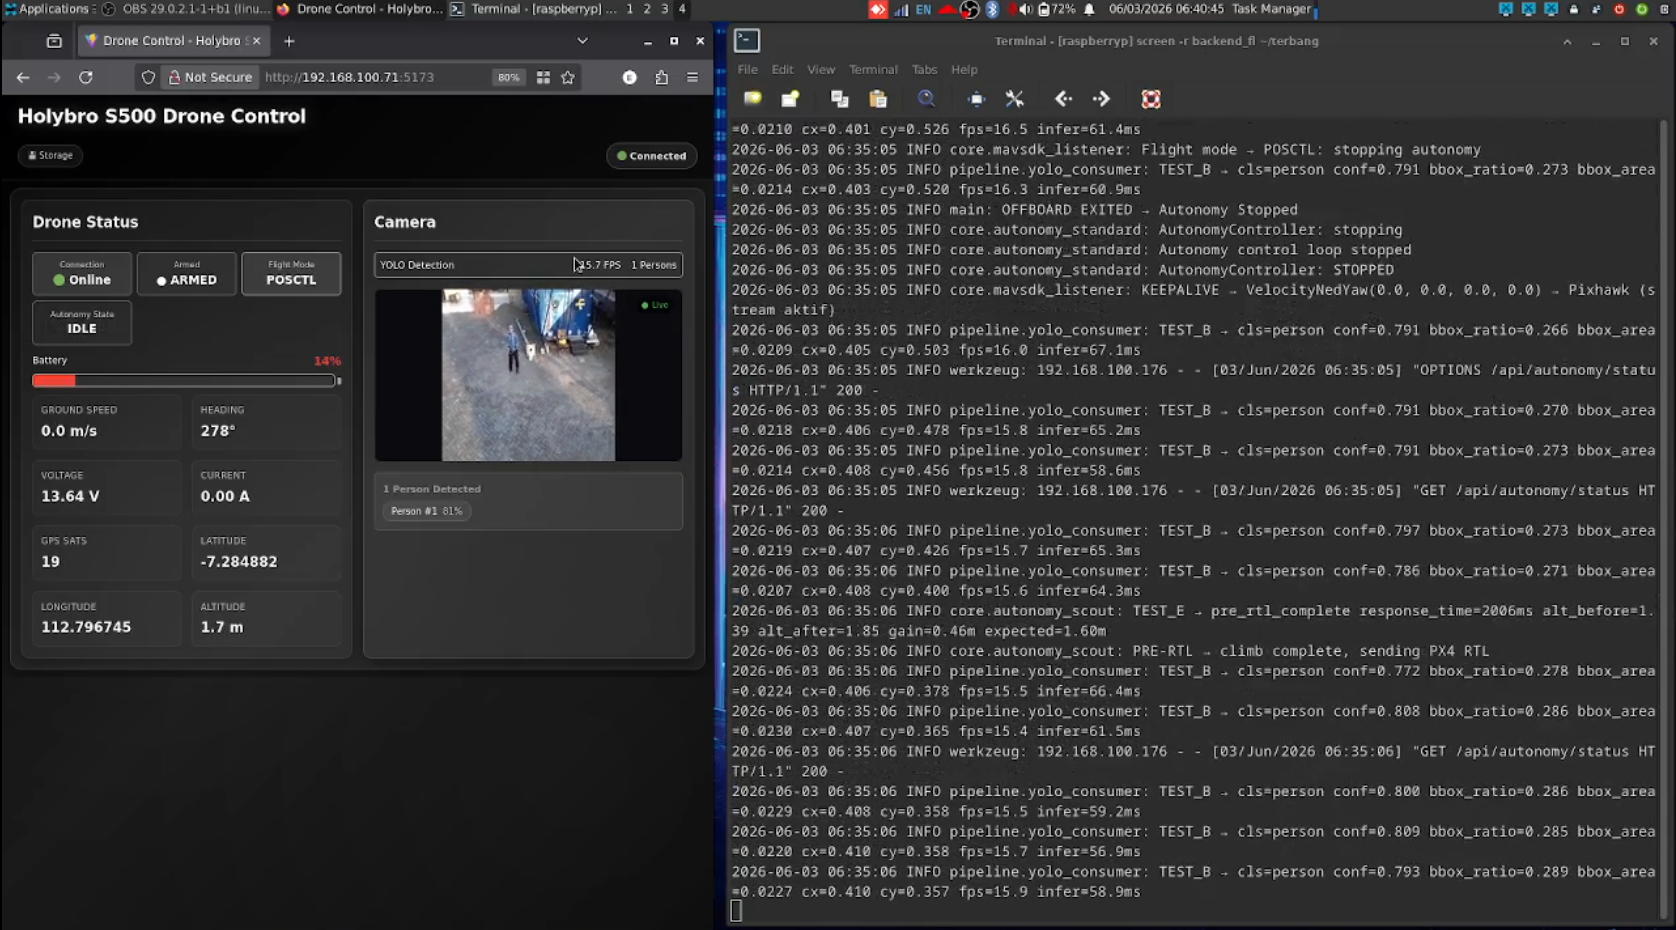
\includegraphics[width=\textwidth]{bab4/preRTLdone_offboardExit}
	\caption{Status Pre-RTL dan OFFBOARD Exit}
	\label{fig:pre_rtl_exit}
\end{figure}

\begin{figure}[H]
	\centering
	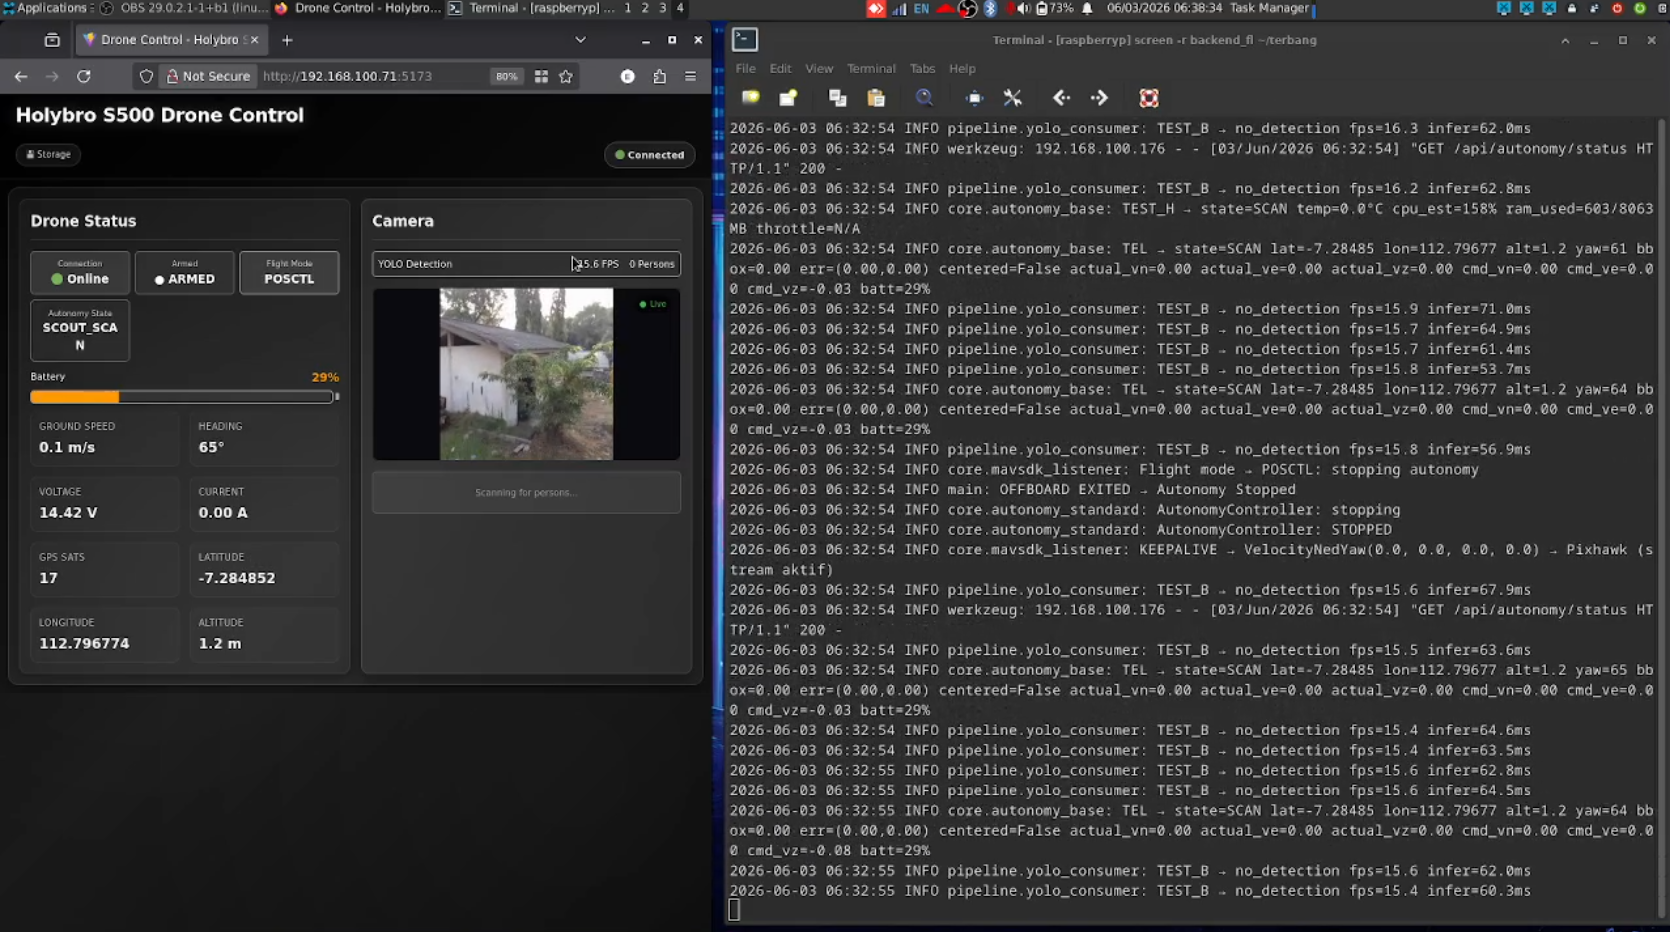
\includegraphics[width=\textwidth]{bab4/rc_override}
	\caption{Intervensi operator (RC Override)}
	\label{fig:rc_override}
\end{figure}

Log keberhasilan aktivasi sistem keselamatan pada Gambar \ref{fig:battery_rtl}, Gambar \ref{fig:pre_rtl_exit}, dan Gambar \ref{fig:rc_override} memverifikasi transisi kontrol yang andal saat terjadi kondisi darurat maupun intervensi manual. Drone secara instan menghentikan misi otonom dan menyerahkan kendali penuh ke pilot tanpa adanya penundaan kontrol yang berisiko, membuktikan ketangguhan sistem pengaman selama misi berlangsung.

\subsection{Skenario F: Pengujian Persistent Multi-Target Scouting}

Pengujian ini bertujuan memvalidasi kemampuan \textit{persistent scouting} untuk melanjutkan pencarian target setelah dokumentasi selesai. Evaluasi juga dilakukan terhadap efektivitas \textit{visited target memory} dan \textit{exclusion radius} dalam mencegah dokumentasi berulang terhadap target yang sama.

Berdasarkan hasil pengujian pada beberapa sesi penerbangan, sistem berhasil mendokumentasikan total 11 target unik dan melakukan 19 kali \textit{duplicate skip} (rekapitulasi hasil pengujian ditunjukkan pada Tabel \ref{tab:scouting_results}). Mekanisme ini memungkinkan UAV untuk tetap melanjutkan proses pencarian target baru tanpa kembali mendokumentasikan target yang telah tersimpan sebelumnya. Pada Flight~1 dan Flight~2 yang berlangsung hingga prosedur \textit{Battery RTL} aktif, sistem berhasil mendokumentasikan masing-masing 3 dan 5 target unik, sekaligus menolak 7 dan 9 kandidat duplikat yang berada dalam area eksklusi. Selain itu, Flight~4 yang melibatkan dua manusia secara bersamaan menunjukkan bahwa sistem mampu melakukan \textit{persistent scouting} terhadap beberapa target dalam satu sesi penerbangan tanpa intervensi operator.

\begin{table}[H]
	\centering
	\caption{Hasil Pengujian Persistent Multi-Target Scouting}
	\label{tab:scouting_results}
	\renewcommand{\arraystretch}{1.2}
	\small
	\resizebox{\textwidth}{!}{
	\begin{tabular}{|c|l|c|c|c|c|c|}
		\hline
		\textbf{Flight \#} &
		\textbf{Skenario} &
		\textbf{Target Ditemukan} &
		\textbf{Duplicate Skipped} &
		\textbf{Total Cycle Time (s)} &
		\textbf{Avg Time per Target (s)} &
		\textbf{Flight Duration (s)}
		\\ \hline
		
		1 &
		Persistent Scouting &
		3 &
		7 &
		170.1 &
		56.7 &
		224
		\\ \hline
		
		2 &
		Persistent Scouting &
		5 &
		9 &
		256.0 &
		51.2 &
		367
		\\ \hline
		
		4 &
		Multi-Target Discovery (2 Persons) &
		2 &
		2 &
		70.0 &
		35.0 &
		70
		\\ \hline
		
		5 &
		Duplicate Validation &
		1 &
		1 &
		81.0 &
		81.0 &
		81
		\\ \hline
		
	\end{tabular}
	}
\end{table}

Pengujian membuktikan mekanisme \textit{persistent scouting} beroperasi sesuai rancangan. Sistem melanjutkan pencarian setelah mendokumentasikan target pertama dengan mengulang siklus \textit{state} dari SCAN, APPROACH, DOCUMENT, hingga DISPLACING secara berulang. Keberhasilan pemicuan \textit{duplicate skip} sebanyak 19 kali memverifikasi peran \textit{visited target memory} dan \textit{exclusion radius} dalam menghindari dokumentasi ulang. Dengan meminimalkan redundansi ini, drone dapat memprioritaskan eksplorasi area baru dan memperluas cakupan pencarian.

\begin{figure}[H]
	\centering
	\begin{subfigure}{0.40\linewidth}
		\centering
		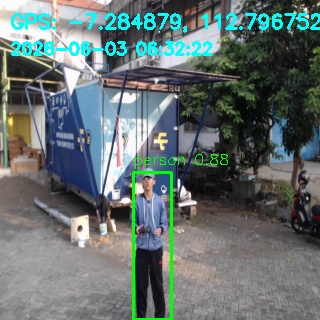
\includegraphics[width=\linewidth]{bab4/scout_20260603_063222_pagidekat}
		\caption{Target Pagi (Dekat)}
	\end{subfigure}
	\hfill
	\begin{subfigure}{0.40\linewidth}
		\centering
		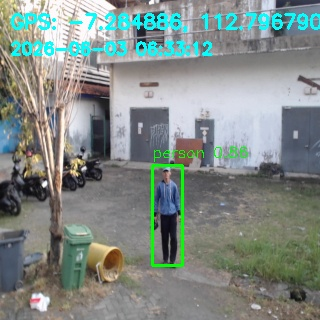
\includegraphics[width=\linewidth]{bab4/scout_20260603_063312_pagijauh}
		\caption{Target Pagi (Jauh)}
	\end{subfigure}
	
	\vspace{0.5cm}
	
	\begin{subfigure}{0.40\linewidth}
		\centering
		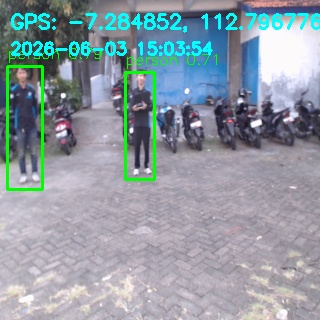
\includegraphics[width=\linewidth]{bab4/scout_20260603_150354_siang}
		\caption{Target Siang}
	\end{subfigure}
	\hfill
	\begin{subfigure}{0.40\linewidth}
		\centering
		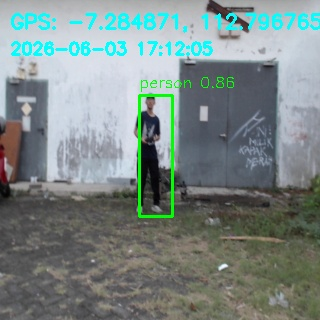
\includegraphics[width=\linewidth]{bab4/scout_20260603_171205_sore}
		\caption{Target Sore}
	\end{subfigure}
	
	\vspace{0.5cm}
	
	\begin{subfigure}{0.40\linewidth}
		\centering
		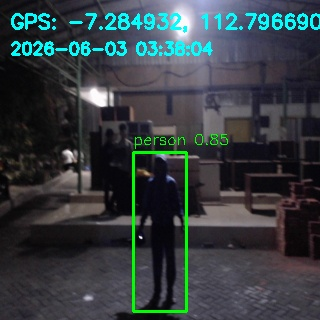
\includegraphics[width=\linewidth]{bab4/scout_20260603_033804_malamterang}
		\caption{Target Malam (Lampu)}
	\end{subfigure}
	\hfill
	\begin{subfigure}{0.40\linewidth}
		\centering
		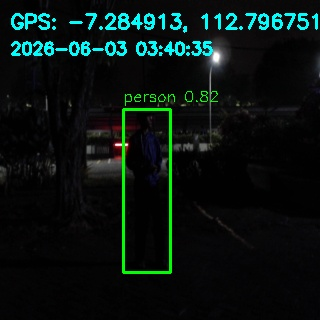
\includegraphics[width=\linewidth]{bab4/scout_20260603_034035_malamgelap}
		\caption{Target Malam (Gelap)}
	\end{subfigure}
	\caption{Dokumentasi target dari pengujian Persistent Scouting}
	\label{fig:persistent_scout}
\end{figure}

Dokumentasi korban selama pengujian misi pencarian otonom ditunjukkan pada Gambar \ref{fig:persistent_scout}. Sistem terbukti mampu mengenali target manusia pada berbagai pose dan kondisi pencahayaan alami di lapangan terbuka dengan kualitas citra yang jelas untuk keperluan verifikasi penyelamatan. Keberhasilan perekaman visual ini melandasi pengujian kestabilan pelacakan target secara dinamis. Bagian berikutnya akan mengevaluasi secara khusus kestabilan penguncian target dan peredaman fluktuasi menggunakan filter koordinat.

\subsection{Skenario G: Pengujian Target Lock Stability \& EMA Smoothing}

Pengujian ini bertujuan untuk memvalidasi kestabilan mekanisme \textit{target locking} serta implementasi \textit{Exponential Moving Average} (EMA) yang digunakan untuk meredam fluktuasi posisi target selama penerbangan. Pengujian dilakukan pada beberapa sesi penerbangan yang melibatkan target bergerak, kemunculan beberapa target secara bersamaan, serta kondisi hilangnya target dari bidang pandang kamera.

Mekanisme pemilihan target menggunakan fungsi penilaian berbasis multi-kriteria yang mengombinasikan luas \textit{bounding box}, tingkat kepercayaan deteksi, posisi relatif terhadap pusat citra, dan histori pelacakan. Setiap target yang dipilih akan menghasilkan log \texttt{lock\_init}, sedangkan target yang kehilangan validitas akan menghasilkan log \texttt{lock\_expired}.

Hasil pengujian pada Tabel \ref{tab:lock_stability} membuktikan kestabilan penguncian target yang tinggi. Selama Flight~1 hingga Flight~4 tidak terjadi peristiwa \texttt{lock\_expired}, sehingga target yang dikunci berhasil dipertahankan untuk dokumentasi. Hanya pada Flight~5 ditemukan satu kali kejadian \texttt{lock\_expired} berdurasi 1,76 detik karena target keluar dari bidang pandang kamera.

\begin{table}[H]
	\centering
	\caption{Hasil Pengujian Target Lock Stability}
	\label{tab:lock_stability}
	\renewcommand{\arraystretch}{1.2}
	\small
	\begin{tabular}{|c|c|c|c|c|}
		\hline
		\textbf{Flight} &
		\textbf{Lock Count} &
		\textbf{Lock Expired} &
		\textbf{Lock Maintained (\%)} &
		\textbf{Avg Lock Duration (s)}
		\\ \hline
		
		Flight 1 & 12 & 0 & 100 & -- \\ \hline
		Flight 2 & 21 & 0 & 100 & -- \\ \hline
		Flight 3 & 1 & 0 & 100 & -- \\ \hline
		Flight 4 & 6 & 0 & 100 & -- \\ \hline
		Flight 5 & 2 & 1 & 50 & 1.76 \\ \hline
		
	\end{tabular}
\end{table}

Selain kestabilan penguncian target, sistem menerapkan \textit{Adaptive Exponential Moving Average} (EMA) untuk pemulusan koordinat target. Faktor pemulusan ($\alpha$) disesuaikan secara dinamis berdasarkan kedekatan target, menggunakan nilai default $\alpha = 0.20$ ketika target berada pada jarak jauh (\textit{bounding box ratio} $\le 0.20$), dan meningkat menjadi $\alpha = 0.30$ ketika target mendekat (\textit{bounding box ratio} $> 0.20$). Peningkatan nilai $\alpha$ pada jarak dekat bertujuan memberikan respons navigasi yang lebih cepat terhadap gerakan dinamis korban, sedangkan nilai $\alpha$ yang lebih rendah pada jarak jauh berguna meredam derau frekuensi tinggi (\textit{jitter}) deteksi. Aktivasi mekanisme filter ini tervalidasi melalui log dengan parameter $\alpha = 0.30$:

\begin{quote}\footnotesize
	\texttt{TEST\_G\_EMA → raw\_cx=... smooth\_cx=... raw\_cy=... smooth\_cy=... alpha=0.30}
\end{quote}

Pengamatan terhadap log menunjukkan bahwa koordinat hasil EMA tersedia dan digunakan selama proses pelacakan berlangsung. Meskipun data log yang tersedia belum cukup rapat untuk melakukan evaluasi statistik jitter secara menyeluruh pada seluruh sesi penerbangan, implementasi EMA berhasil beroperasi secara konsisten tanpa menyebabkan hilangnya target maupun perpindahan kunci target yang tidak diperlukan.

Pengujian membuktikan mekanisme \textit{target locking} dapat mempertahankan target secara stabil dalam kondisi riil, termasuk saat terdapat beberapa kandidat objek. Ketiadaan perpindahan kunci target secara tidak sengaja (\textit{unnecessary lock switching}) menunjukkan konsistensi navigasi otonom yang tinggi. Evaluasi kebutuhan komputasi onboard untuk menjaga kontinuitas performa ini dipaparkan pada subbab berikutnya.

\subsection{Skenario H: Pengujian Performa Termal dan Resource saat Penerbangan}

Pengujian ini bertujuan untuk mengevaluasi konsumsi sumber daya komputasi Raspberry Pi 5 selama menjalankan misi otonom secara penuh. Monitoring dilakukan secara periodik setiap 5 detik melalui log \texttt{TEST\_H} yang mencatat state aktif sistem, estimasi utilisasi CPU, penggunaan RAM, temperatur sistem, serta status \textit{thermal throttling}.

Beban komputasi selama penerbangan (Tabel \ref{tab:resource_monitoring}) tergolong tinggi karena eksekusi paralel dari pipa video GStreamer, inferensi YOLOv8n (ONNX Runtime), komunikasi MAVSDK, kontrol otonom, dan dasbor web. Utilisasi CPU rata-rata selama misi mencapai 144,06\% dengan puncak 177\%, mengindikasikan penggunaan multi-inti secara simultan.

Penggunaan memori selama penerbangan juga menunjukkan kondisi yang stabil. Konsumsi RAM rata-rata berada pada rentang sekitar 600 MB dari total kapasitas fisik 8 GB, tanpa ditemukan indikasi peningkatan penggunaan memori secara terus-menerus yang mengarah pada \textit{memory leak}. Selama seluruh pengujian, tidak ditemukan kejadian \textit{thermal throttling} yang tercatat pada log sistem.

Analisis performa termal dilakukan secara kualitatif berdasarkan pemantauan status \textit{throttling} internal perangkat keras Raspberry Pi 5. Selama keseluruhan misi berlangsung, tidak ditemukan satupun indikasi \textit{thermal throttling} maupun pelambatan frekuensi \textit{clock} komputasi, yang membuktikan bahwa disipasi termal bawaan sudah cukup andal dalam menahan beban suhu operasional penuh.

\begin{table}[H]
	\centering
	\caption{Hasil Pengujian Performa Termal dan Resource saat Penerbangan}
	\label{tab:resource_monitoring}
	\renewcommand{\arraystretch}{1.2}
	\small
	\resizebox{\textwidth}{!}{
	\begin{tabular}{|l|c|c|c|c|}
		\hline
		\textbf{Phase} &
		\textbf{Avg CPU (\%)} &
		\textbf{Peak CPU (\%)} &
		\textbf{Avg RAM (MB)} &
		\textbf{Throttle Events}
		\\ \hline
		
		SCAN &
		145.45 &
		177 &
		599.69 &
		0
		\\ \hline
		
		APPROACH &
		141.41 &
		174 &
		604.66 &
		0
		\\ \hline
		
		DISPLACING &
		142.69 &
		172 &
		599.62 &
		0
		\\ \hline
		
		Full Mission Average &
		144.06 &
		177 &
		600.57 &
		0
		\\ \hline
		
	\end{tabular}
	}
\end{table}

Hasil pengujian menunjukkan bahwa Raspberry Pi 5 mampu menjalankan seluruh komponen sistem otonom secara bersamaan tanpa mengalami kegagalan proses maupun kejadian \textit{throttling} yang terdeteksi. Meskipun beban CPU relatif tinggi akibat inferensi visi komputer yang berjalan terus-menerus selama misi, penggunaan RAM tetap rendah dibandingkan kapasitas total sistem, sehingga masih tersedia ruang sumber daya yang cukup untuk pengembangan fitur tambahan pada implementasi berikutnya. Kestabilan performa termal ini mendukung keberlanjutan operasi komputasi di bawah berbagai kondisi lingkungan. Skenario pengujian terakhir mengevaluasi ketahanan deteksi visual di bawah pengaruh fluktuasi intensitas cahaya matahari dan kegelapan malam.

\subsection{Skenario I: Pengujian Ketahanan Lingkungan (Environmental Robustness)}

Pengujian \textit{environmental robustness} dilakukan untuk mengevaluasi pengaruh variasi kondisi pencahayaan terhadap performa deteksi manusia dan kemampuan operasi sistem otonom. Pengujian dilaksanakan pada beberapa sesi penerbangan dengan kondisi waktu berbeda, yaitu subuh (Flight~1), pagi (Flight~2 dan Flight~3), siang (Flight~4), serta sore (Flight~5).

Hasil pengujian menunjukkan bahwa performa deteksi sangat dipengaruhi oleh kualitas pencahayaan lingkungan. Pada kondisi siang hari (Flight~4), sistem memperoleh tingkat deteksi tertinggi sebesar 78,58\% dengan FPS rata-rata 16,11 FPS. Kondisi ini memberikan pencahayaan paling merata sehingga model YOLOv8n dapat menghasilkan deteksi yang lebih konsisten.

Sebaliknya, pada kondisi subuh (Flight~1) dan sore (Flight~5), tingkat deteksi mengalami penurunan signifikan menjadi 24,04\% dan 26,46\%. Berdasarkan observasi lapangan, kondisi ini dipengaruhi oleh rendahnya intensitas cahaya yang diterima sensor kamera sehingga kualitas citra menurun dan proses \textit{autofocus} kamera menjadi kurang stabil. Walaupun demikian, model masih mampu menghasilkan nilai \textit{confidence} rata-rata di atas 0,78 pada seluruh kondisi pengujian.

Hasil ini menunjukkan bahwa sistem mampu beroperasi dengan baik pada kondisi \textit{daylight outdoor}, namun performa deteksi menurun pada kondisi pencahayaan rendah. Temuan ini sekaligus menguatkan batasan penelitian yang membatasi penggunaan sistem pada lingkungan luar ruang dengan pencahayaan memadai.

\begin{table}[H]
	\centering
	\caption{Pengaruh Kondisi Cahaya terhadap Performa Deteksi}
	\label{tab:env_light}
	\renewcommand{\arraystretch}{1.2}
	\small
	\resizebox{\textwidth}{!}{
	\begin{tabular}{|l|c|c|c|p{4.5cm}|}
		\hline
		\textbf{Waktu} &
		\textbf{Avg Confidence} &
		\textbf{Detection Rate (\%)} &
		\textbf{FPS avg} &
		\textbf{Catatan}
		\\ \hline
		
		Subuh (Flight~1) &
		0.783 &
		24.04 &
		14.98 &
		Pencahayaan rendah, deteksi tidak konsisten
		\\ \hline
		
		Pagi (Flight~2--3) &
		0.806 &
		45.31 &
		16.19 &
		Kondisi pencahayaan cukup stabil
		\\ \hline
		
		Siang (Flight~4) &
		0.781 &
		78.58 &
		16.11 &
		Performa deteksi terbaik
		\\ \hline
		
		Sore (Flight~5) &
		0.811 &
		26.46 &
		16.26 &
		Deteksi menurun akibat berkurangnya intensitas cahaya
		\\ \hline
		
	\end{tabular}
	}
\end{table}

Berdasarkan data pada Tabel~\ref{tab:env_light} dan perbandingan visual pada Gambar \ref{fig:environmental_robustness}, tingkat keberhasilan deteksi YOLOv8n hasil \textit{fine-tuning} dipengaruhi oleh intensitas cahaya lingkungan. Performa mencapai titik optimal pada siang hari karena pencahayaan yang merata meminimalisir bayangan dan derau (\textit{noise}) visual pada citra. Sebaliknya, pada kondisi subuh dan sore, tingkat deteksi menurun akibat rendahnya intensitas cahaya yang mempersulit stabilisasi fokus kamera. Limitasi ekstrem terjadi pada malam gelap tanpa bantuan cahaya buatan, di mana model gagal mengenali target akibat hilangnya fitur visual manusia secara total. Meskipun demikian, iluminasi lampu sorot atau lampu jalan terbukti dapat memulihkan deteksi secara terbatas. Dengan demikian, sistem otonom ini memenuhi tujuan perancangan untuk beroperasi pada lingkungan luar ruang dengan pencahayaan memadai (\textit{daylight condition}), namun memerlukan dukungan pencahayaan tambahan jika digunakan untuk operasi minim cahaya.

\begin{figure}[H]
	\centering
	\begin{subfigure}{\textwidth}
		\centering
		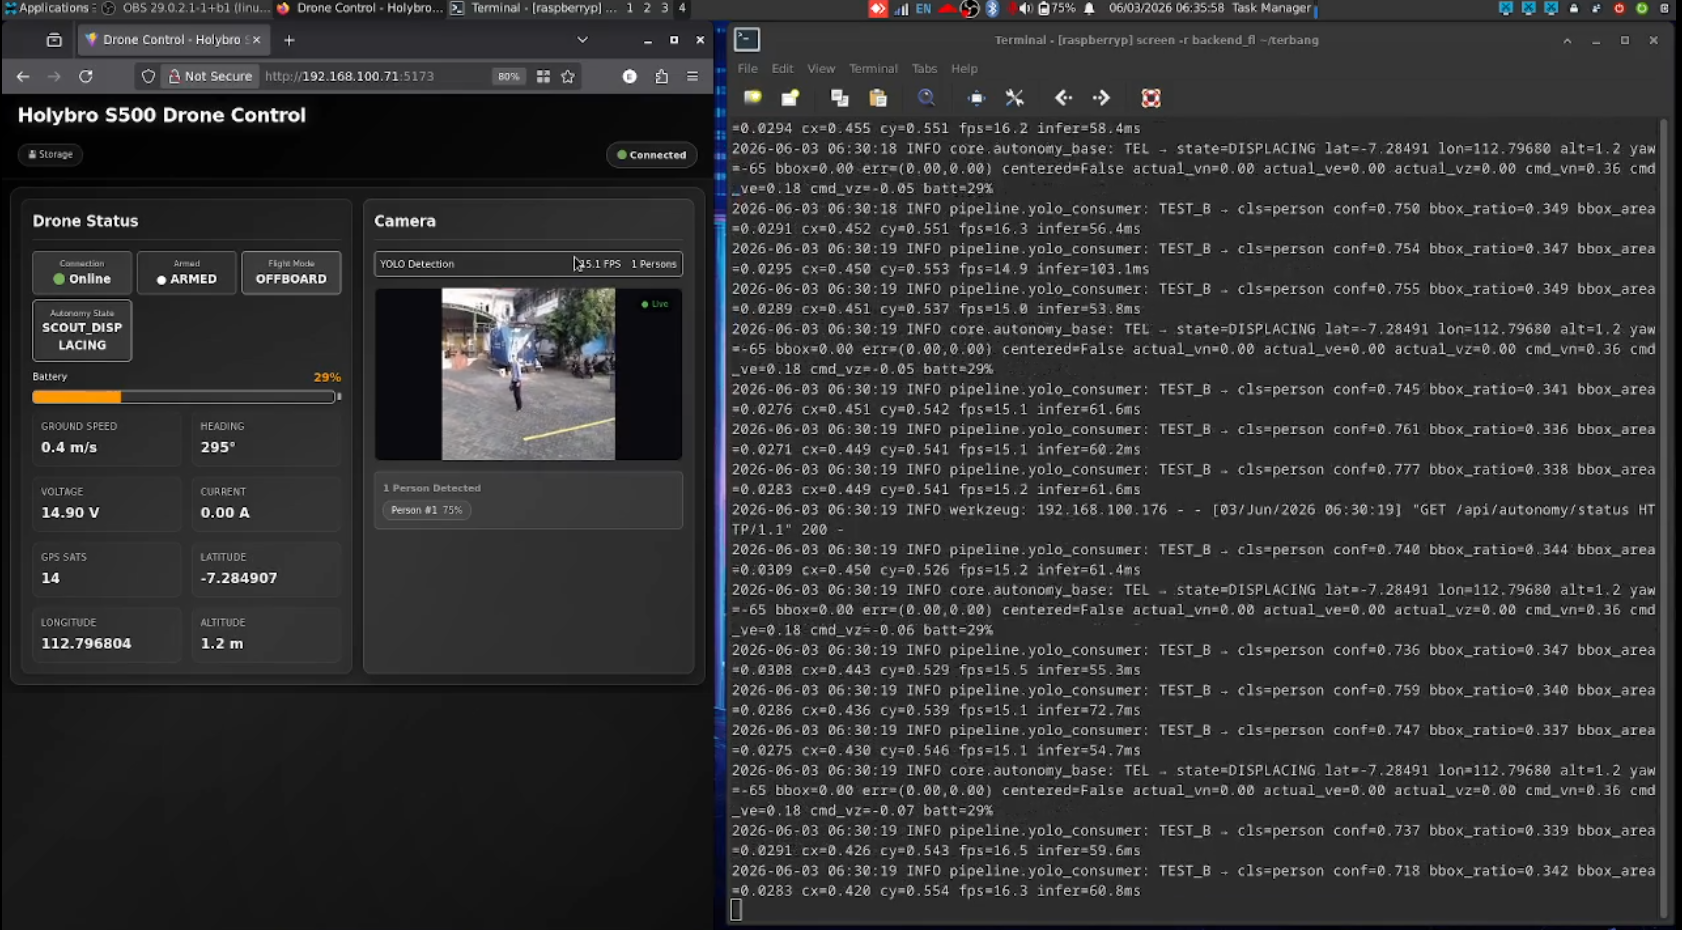
\includegraphics[width=\textwidth]{bab4/terbang_pagi}
		\caption{Kondisi Pagi}
	\end{subfigure}
	\hfill
	\begin{subfigure}{\textwidth}
		\centering
		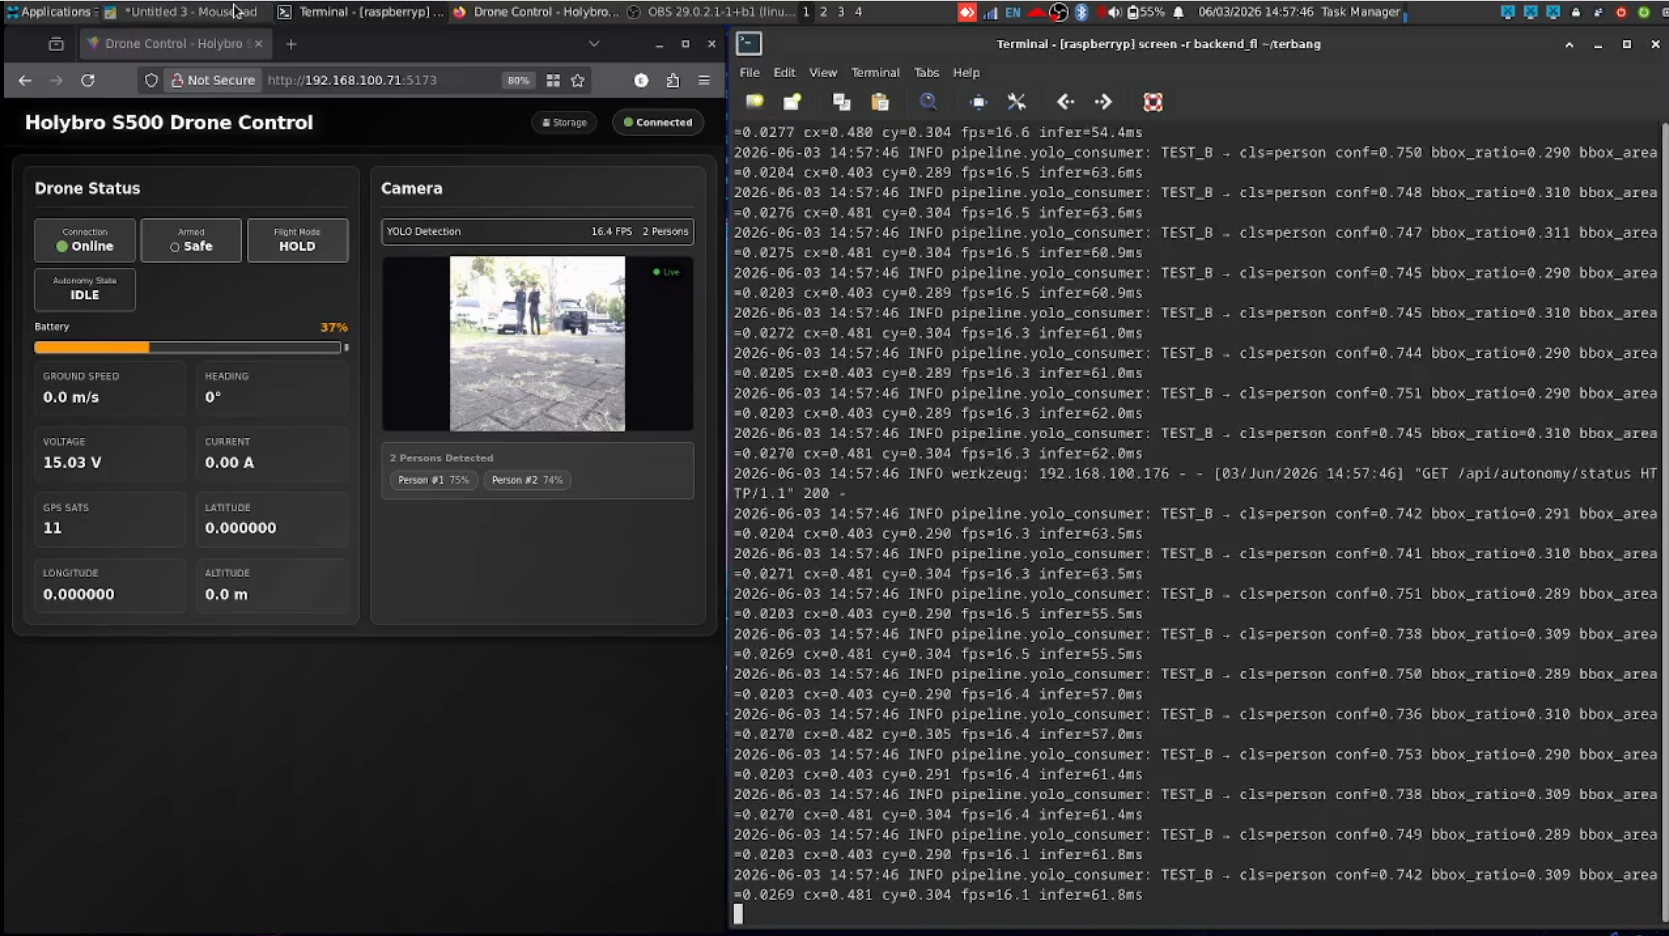
\includegraphics[width=\textwidth]{bab4/terbang_siang}
		\caption{Kondisi Siang}
	\end{subfigure}
	\caption{Perbandingan deteksi pada berbagai kondisi pencahayaan}
	\label{fig:environmental_robustness}
\end{figure}

\begin{figure}[H]
	\ContinuedFloat
	\centering
	\begin{subfigure}{\textwidth}
		\centering
		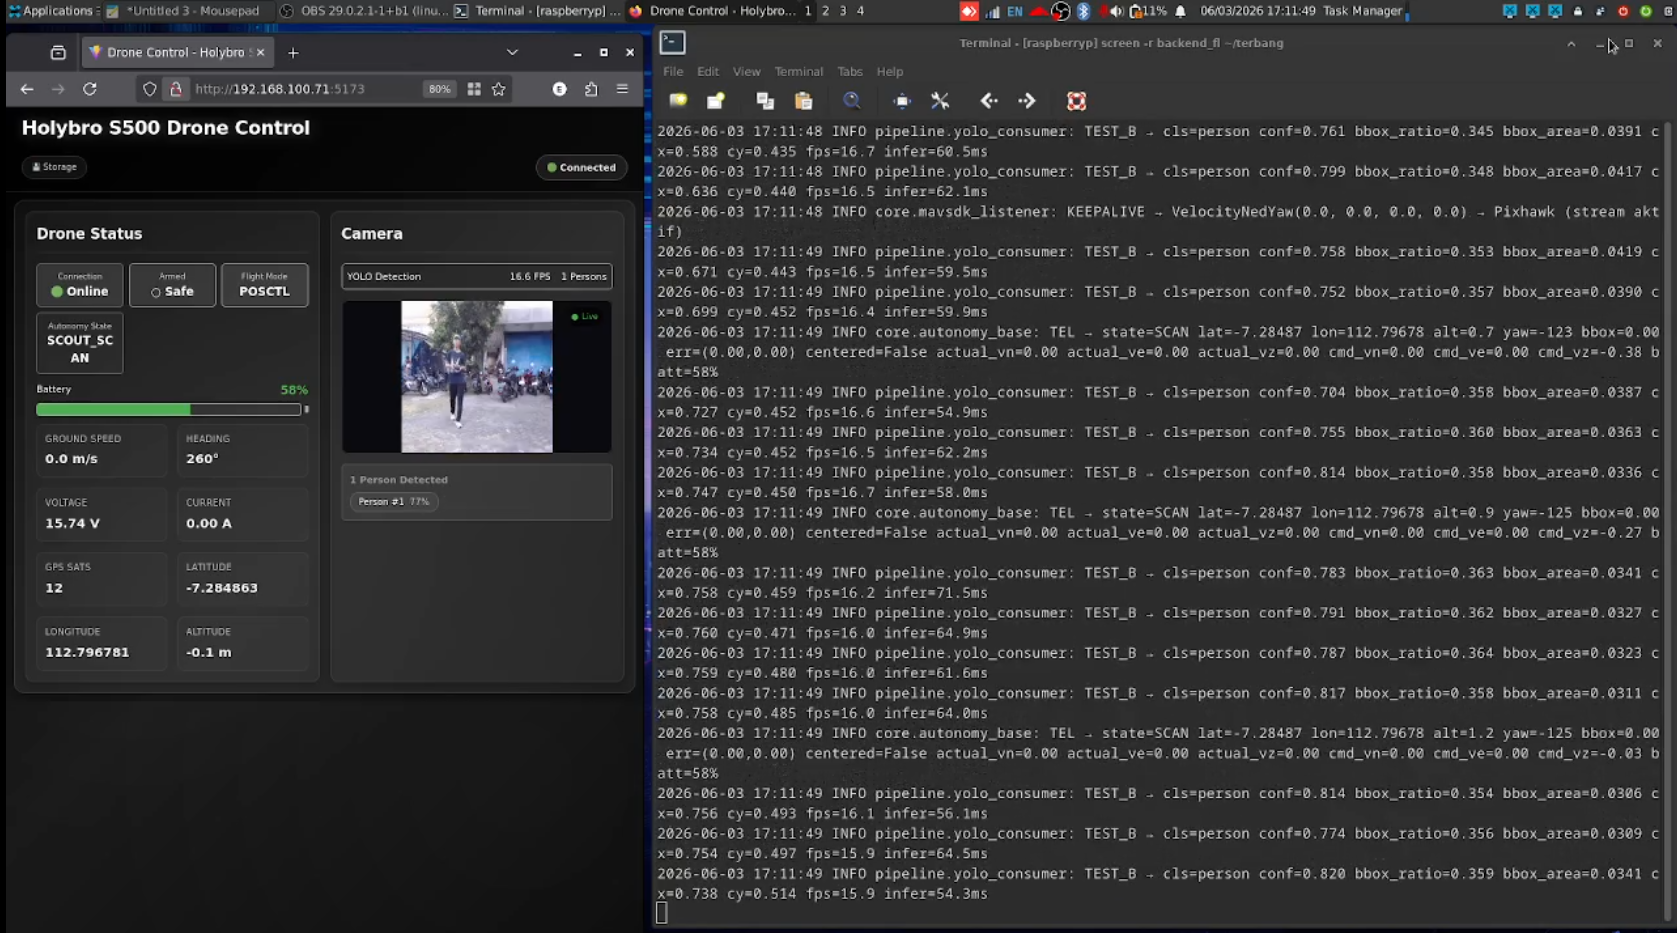
\includegraphics[width=\textwidth]{bab4/terbang_sore}
		\caption{Kondisi Sore}
	\end{subfigure}
	\hfill
	\begin{subfigure}{\textwidth}
		\centering
		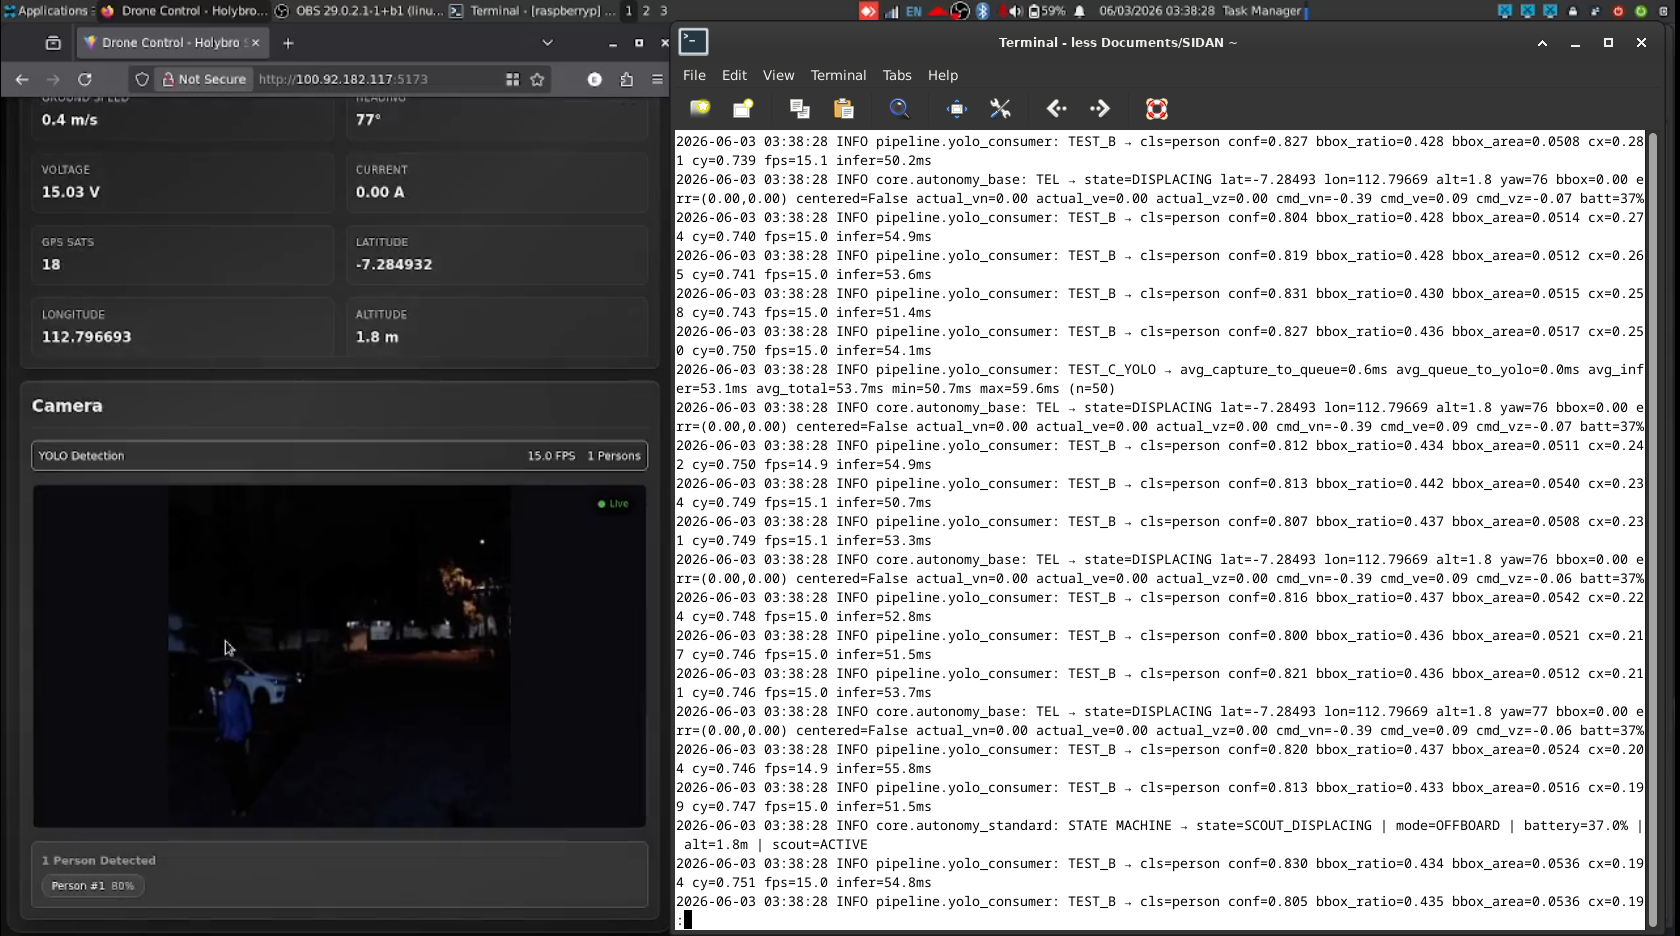
\includegraphics[width=\textwidth]{bab4/terbang_malam_manusia}
		\caption{Kondisi Malam (dengan iluminasi lampu)}
	\end{subfigure}
	\caption{Perbandingan deteksi pada berbagai kondisi pencahayaan (Lanjutan)}
\end{figure}

\begin{figure}[H]
	\ContinuedFloat
	\centering
	\begin{subfigure}{\textwidth}
		\centering
		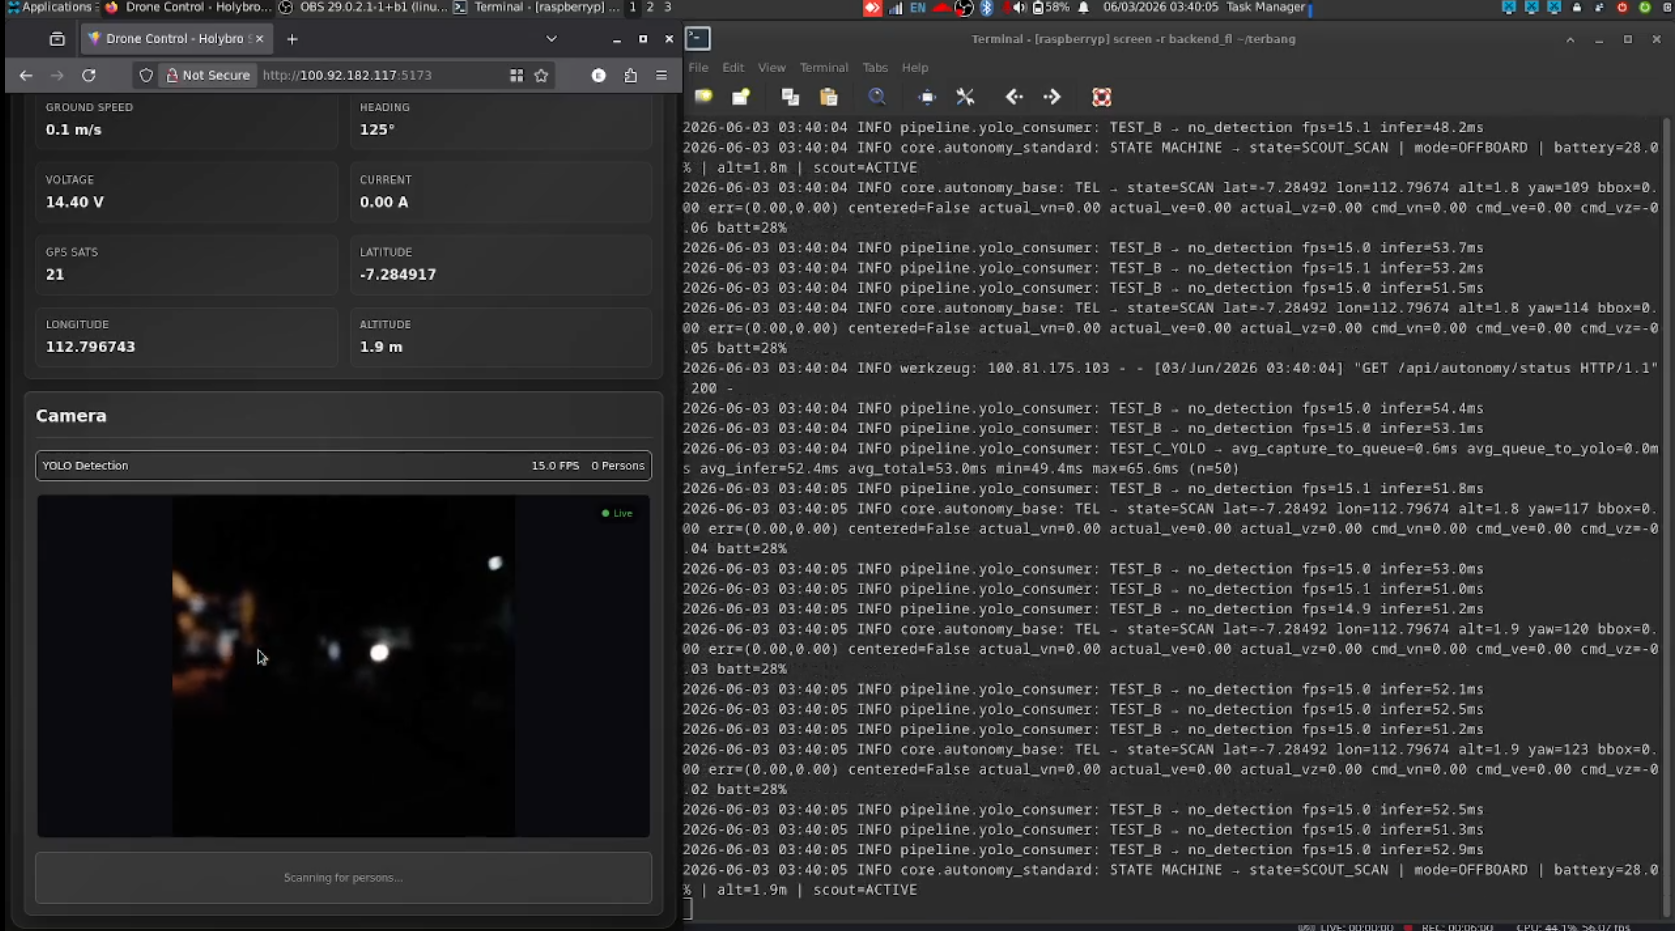
\includegraphics[width=\textwidth]{bab4/terbang_malam_gelap}
		\caption{Kondisi Malam Gelap}
	\end{subfigure}
	\caption{Perbandingan deteksi pada berbagai kondisi pencahayaan (Lanjutan)}
\end{figure}

Seluruh hasil pengamatan terhadap ketahanan visual model deteksi di bawah berbagai tingkat iluminasi cahaya luar ruang tersebut menyimpulkan rangkaian aktivitas validasi sistem drone otonom. Hasil observasi dan analisis komparatif ini selanjutnya dikumpulkan untuk mengevaluasi tingkat keberhasilan sistem secara menyeluruh terhadap tujuan penelitian.

\section{Evaluasi Keberhasilan Sistem}

Berdasarkan keseluruhan tahapan pengujian, sistem drone otonom pendeteksi manusia berbasis \textit{edge computing} ini dinyatakan berhasil menjawab rumusan masalah dan mencapai tujuan penelitian. Sistem terbukti mampu menjalankan operasi pencarian korban secara \textit{real-time} tanpa intervensi manual berkat integrasi arsitektur perangkat lunak yang dirancang secara asinkron antara \textit{backend} inferensi YOLOv8n, komunikasi telemetri MAVSDK, dan antarmuka pemantauan \textit{frontend} React.

Pemilihan arsitektur deteksi YOLOv8n yang dikonversi ke format ONNX dengan resolusi input 320$\times$320 piksel, serta dijalankan pada sistem operasi \textit{headless}, terbukti menjadi titik keseimbangan yang optimal. Konfigurasi ini sukses menjaga latensi \textit{end-to-end} konsisten di bawah 200 ms dan rata-rata FPS di kisaran 16-23 Hz, sama sekali mengeliminasi insiden \textit{bottleneck} pada prosesor Raspberry Pi 5.

Penelitian ini juga mendemonstrasikan kontribusi desain melalui logika otonom \textit{Persistent Multi-Target Scouting}. Dukungan memori target historis dan mekanisme eksklusi radius berbasis komputasi jarak \textit{Haversine} memungkinkan drone untuk terus menjelajah (\textit{displace} dan \textit{scan} ulang) tanpa terjebak pada subjek yang sudah terekam. Pendekatan ini meningkatkan efisiensi operasional SAR secara drastis dibandingkan dengan siklus \textit{Return to Launch} setelah satu temuan. Di aspek redundansi pengamanan, arsitektur keselamatan tiga lapis (\textit{Three-Layer Safety System}) sukses melakukan pencegahan kecelakaan terbang rendah dengan fitur \textit{Pre-RTL Safety Climb} sejauh $\sim$2 meter setiap kali mode pembatalan akibat baterai kritis dipicu.

Meskipun demikian, sistem cerdas ini memiliki batasan yang menjadi temuan evaluasi. Uji keandalan paparan lingkungan (\textit{environmental robustness}) menegaskan bahwa performa deteksi jatuh drastis pada petang atau subuh (di bawah 30\%) akibat absennya sumber pencahayaan inframerah pasif. Sistem juga menyingkirkan implementasi fitur estimasi pose tubuh lengan/kaki karena mengacaukan stabilitas \textit{frame} saat dioperasikan di lapangan terbuka (\textit{outdoor}). Pada aspek komunikasi, penggunaan jaringan MiFi 4G/5G memicu penumpukan aliran video (\textit{stuttering}) pada antarmuka \textit{dashboard} ketika sinyal terhalang struktur fisik di lapangan, meskipun eksekusi komputasi \textit{edge processing} di dalam drone terbukti kebal dari gangguan latensi tersebut. Keterbatasan-keterbatasan ini membuka dimensi bagi penelitian lanjutan seperti penyematan kamera termal untuk pencarian malam hari, penerapan teknik algoritma kompresi video adaptif berlatensi rendah, serta fusi sensor spasial untuk meredam pelacakan semu akibat rintangan vegetasi.